\documentclass[10pt]{article}
\usepackage{microtype}
\usepackage{graphicx}
\usepackage{subcaption}
\usepackage{booktabs}
\usepackage{xurl}
\usepackage{hyperref}
\usepackage[T1]{fontenc}
\usepackage{tmlr}
\usepackage{amsmath,amssymb,amsfonts,mathtools}
\usepackage{amsthm}
\usepackage{placeins}
\usepackage{float}
\usepackage{needspace}
\usepackage[nameinlink,capitalize,noabbrev]{cleveref}
\newcommand{\R}{\mathbb{R}}
\newcommand{\Id}{\mathbf{I}}
\newcommand{\norm}[1]{\left\lVert #1\right\rVert}
\newcommand{\Eeq}{E_{\mathrm{eq}}}
\newcommand{\Ehom}{E_{\mathrm{hom,data}}}
\newcommand{\Ehomop}{E_{\mathrm{hom,op}}}
\newcommand{\Erel}{E_{\mathrm{rel,data}}}
\newcommand{\Erelop}{E_{\mathrm{rel,op}}}
\newcommand{\Ecomp}{E_{\mathrm{comp,data}}}
\newcommand{\Ecompop}{E_{\mathrm{comp,op}}}
\newtheorem{proposition}{Proposition}
\newtheorem{corollary}[proposition]{Corollary}
\newtheorem{spectraltheorem}[proposition]{Theorem}
\newtheorem{spectrallemma}[proposition]{Lemma}
\crefname{spectraltheorem}{Theorem}{Theorems}
\crefname{spectrallemma}{Lemma}{Lemmas}
\title{Beyond Shared Geometry: Predictive Recovery,\\
Exact Actions, and Registration Preference\\
in Language-Model Representations}
\author{Anonymous authors}
% Generated from full precision cell rows.
\newcommand{\BoundedIdentityCseven}{0.76012}
\newcommand{\BoundedPremiumLowerCseven}{0.00416}
\newcommand{\BoundedPremiumUpperCseven}{0.03300}
\newcommand{\BoundedPositiveCseven}{24}
\newcommand{\BoundedUniqueCseven}{7}
\newcommand{\BoundedTiedCseven}{0}
\newcommand{\BoundedBehindCseven}{17}
\newcommand{\BoundedIdentityDfour}{0.52932}
\newcommand{\BoundedPremiumLowerDfour}{0.02624}
\newcommand{\BoundedPremiumUpperDfour}{0.14574}
\newcommand{\BoundedPositiveDfour}{24}
\newcommand{\BoundedUniqueDfour}{16}
\newcommand{\BoundedTiedDfour}{0}
\newcommand{\BoundedBehindDfour}{8}
\newcommand{\BoundedAllPositive}{48}
\newcommand{\BoundedCellCount}{48}
\newcommand{\BoundedCellsPerDomain}{24}
\newcommand{\BoundedIdentityMaxError}{$3.77\!\times\!10^{-15}$}
\newcommand{\BoundedScalarAtol}{$1.00\!\times\!10^{-8}$}
\newcommand{\BoundedScalarRtol}{$1.00\!\times\!10^{-7}$}

\begin{document}
\maketitle
% Retain the official TMLR page-bottom alignment.

\begin{abstract}
Predictive maps between language-model representations need not identify the transformation structure those representations support. We study finite-group actions on visible input states with coordinates shared across contexts. A spectral budget retaining complete real irreducible components bounds the minimum prediction risk over exact orthogonal actions of a fixed real dimension. Under a common second-moment-whitened loss, its upper endpoint is at most twice its lower endpoint. An analytical example shows that the ordinary orbit-Gram spectrum does not determine this exact-action risk. On fixed banks from six frozen Llama and Qwen models, we separate independent orthogonality cost from bounds on the further cost of common group laws. These finite-bank class comparisons are distinct from held-out prediction. Training-constructed exact actions predict held-out representations less accurately than training-fitted independent least squares. Spectral registration preference depends on retained dimension and state-invariant components. At dimension 16, within-template centering with the original whitening changes the prescribed image's unique leads from 7/24 to 15/24 weekday ($C_7$) conditions and from 16/24 to 0/24 corner ($D_4$) conditions. Rewhitening raises the weekday count to 18/24 while corners remain at 0/24. On separately authored contexts, difference fitting lowers mean weekday error and raises mean corner error relative to coordinate fitting; wording, validation selection and, for corners, action weighting also differ from the earlier protocol. These comparisons distinguish predictive transport, fixed-bank exact-action compatibility and spectral preference from evidence of native computation.
\end{abstract}

\section{Introduction}
Equivariance describes how a learned representation responds to input transformations.
Let $f(x)$ denote the hidden representation extracted from the model for input $x$.
Let $G$ act on the inputs and let $\rho$ be an action of $G$ on the representation space.
The map $f$ is equivariant with respect to $\rho$ if $f(g\cdot x)=\rho(g)f(x)$ for every $g\in G$ and every input $x$.
In other words, the hidden representation of the transformed input equals the result of applying $\rho(g)$ to the original hidden representation.
The maps $\rho(g)$ compose according to the same group law as the input transformations by definition.
Prior work fits maps to paired representations \citep{lenc2015understanding} and studies when a transformation induces a well-defined map on the encoder's image \citep{sun2026transformationlaws}.
One approach is to learn the representation space and the group action jointly \citep{schmidt2025equivariance}.
We study how closely the existing hidden representations of a frozen language model can satisfy the equivariance relation for a prescribed group of input transformations.
On a fixed set of representations, we bound the minimum prediction error over exact orthogonal actions.
Under a common loss, we compare these bounds with the minima for independently chosen linear and orthogonal maps to separate the cost of orthogonality from the additional cost of enforcing the group law.
A low error under these constraints means that an exact action can closely predict the effects of the prescribed transformations on the representations.
The same representations may also support alternative actions that obey the same group laws but map states to different targets.
We therefore hold the representations fixed and compare the spectral budget of the prescribed action with those of the alternatives to assess whether the prescribed state correspondences receive stronger support.

We study two families of transformations on states named in the input.
In the weekday task, a one-day shift takes ``The current day is Monday.'' to ``The current day is Tuesday.''
Seven successive shifts return each day to itself, giving the cyclic group $C_7$.
In the square-corner task, a clockwise quarter turn takes NW to NE, while a reflection across the NW--SE diagonal fixes NW and SE and swaps NE with SW.
The rotations and reflections form the dihedral group $D_4$.
In both tasks, different state correspondences can obey the same group laws.
For example, swapping the positions of Tuesday and Wednesday in the weekday cycle changes Monday's successor to Wednesday while preserving the seven-step return.

Figure~\ref{fig:evaluation-targets} shows what changes in each evaluation.
For prediction, we fit maps on training templates and test them on held-out templates with the same state vocabulary.
The structural recovery and coordinate studies use separately constructed sets of templates and different prediction losses.
On each complete test bank in the coordinate study, we assess the cost of imposing exact action constraints while holding the representations, target pairs, and loss fixed.
We then compare the prescribed action with alternatives by changing the target pairs and computing the spectral budget of each action on the same bank.

% Keep the evaluation diagram near its first reference.
\begin{figure}[!htbp]
\centering
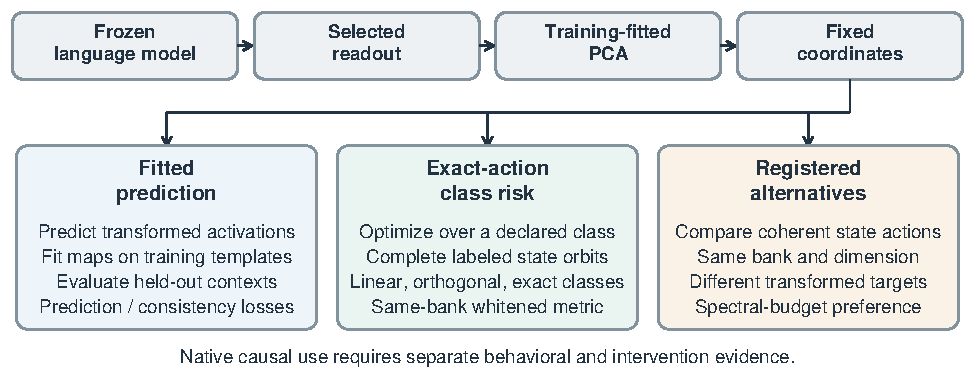
\includegraphics[width=\linewidth]{figures/evaluation_targets.pdf}
\caption{Three evaluation questions illustrated for a given bank of fixed representations. Fitted prediction scores learned maps on held-out contexts. Exact-action analysis bounds a class optimum in a declared metric. Registration comparisons change the coherent target action while keeping the source bank fixed. Each branch has its own evidence requirements.}
\label{fig:evaluation-targets}
\end{figure}

Our main theorem bounds the minimum prediction error $L^\star$ over exact orthogonal actions in a fixed real dimension $r$.
We compute a spectral budget from the orbit Gram matrix of the whitened representations and the group's action on its blocks.
The budget is the largest fraction of orbit energy that an invariant subspace of at most $r$ dimensions can capture.
The subspace must retain whole real irreducible components, so a two-dimensional rotation plane uses two dimensions of the budget.
In a constructed example, two systems have identical orbit-Gram eigenvalues and hence the same minimum error for independent linear maps.
Those eigenvalues belong to two one-dimensional components in one system and to a single two-dimensional rotation plane in the other.
With only one dimension available, the two systems have different minimum errors under exact orthogonal actions.
The spectral budget accounts for this difference and gives an upper bound on $L^\star$ that is at most twice the lower bound.

We evaluate both tasks in six frozen Llama and Qwen models.
In the structural recovery study, fitted linear maps reduce prediction error on held-out templates relative to the identity baseline.
In the coordinate study, the lower bounds on the additional cost of enforcing the group law beyond orthogonality vary widely across model and layer conditions.
In the 16-dimensional weekday analysis, a single condition accounts for 99.44\% of the sum of these lower bounds.
At the same dimension, the spectral budget of the prescribed action exceeds that of every alternative by more than the comparison tolerance in 7 of 24 weekday conditions and 16 of 24 square-corner conditions.
Reducing the retained dimension to eight changes both counts.

We also evaluate exact orthogonal actions constructed from training contexts as predictors on held-out contexts.
In every evaluated condition, the constructed action has higher prediction error than ordinary least squares fitted on the same training contexts.
A separate experiment evaluates two fitting objectives on newly authored context pairs containing the same state vocabulary.
We fit both predictors on the original training contexts, one to individual representations and the other to differences between paired representations of the same state.
We score both on their predictions of representation differences in the new pairs.
Relative to fitting individual representations, fitting differences lowers mean prediction error for weekdays and raises it for square corners.
Determining whether the model uses these transformations to compute its outputs would require behavioral and intervention evidence.

% Keep the introduction diagram before Related Work, without a fixed page number.
\FloatBarrier

\section{Related Work}
\label{sec:related-main}
\paragraph{Measuring transformations in learned representations.}
\citet{lenc2015understanding} fit maps between representations of paired images to measure how features respond to input transformations, and use related mappings for network stitching.
\citet{gruver2023lie} use the Lie derivative to measure how closely learned visual representations respect continuous input transformations.
In language models, \citet{hernandez2024linearity} find that affine maps derived from model Jacobians approximate subject-to-object decoding for some relations.
We fit maps for prescribed finite groups, where we can also test whether the fitted maps compose as the input transformations do.

\paragraph{Sharing a map and satisfying a group law.}
\citet[arXiv v1, Sections~III and V]{sun2026transformationlaws} characterizes when an input transformation induces a well-defined map on the image of an encoder.
Sun separates local fitting error for a given transformation from the cost of sharing one map across regions defined by the encoder's activation patterns. The preprint compares global and local maps on frozen visual features.
In our setting, each group element already uses a map shared across contexts. We give spectral bounds on the minimum prediction error in a fixed dimension when these maps must be orthogonal and jointly obey the group law exactly.
In frozen language models, we also compare the prescribed way of transforming the input states with alternative ways that obey the same group laws.

\paragraph{Learning equivariant representations.}
The Homomorphism AutoEncoder learns representations and actions jointly from transitions \citep{keurti2023homomorphism}.
Under its generative and diversity assumptions, Equivariance by Contrast identifies jointly learned representations and actions up to a common invertible change of coordinates \citep{schmidt2025equivariance}.
We take the hidden representations and the action on the input states as given. The maps that predict changes in those representations are the objects of comparison.

\paragraph{Spectral approximation and constraint costs.}
Prior work uses spectral methods to approximate data in group-invariant spaces or to learn features subject to symmetry constraints \citep{barbieri2020approximation,koyama2024fourier,ordonez2026inference}.
We use the energy that can be retained in whole symmetry components to bound the best prediction error at a given dimension.
\citet{wang2023equivariance} bound equivariant regression error when both the input and output actions are prescribed. Our bounds allow the action on the hidden representations to vary.
\citet{elesedy2021generalisation} analyze expected test error under symmetry assumptions. We report the cost of the constraints by comparing minimum errors on one fixed set of observed representations and assess generalization in separate held-out comparisons.

\paragraph{Shared geometry.}
\citet{hu2026language} report shared geometry across language models both in how concepts are represented and in how their representations shift with context. They use displacements in one model to help predict held-out displacements in another.
\citet{wurgaft2026manifold} connect activation geometry to output behavior by steering along fitted manifolds.
Our main comparisons change a state named in the input within a fixed model and context template. We ask how well an exact group action captures those changes and whether the prescribed state correspondences receive stronger support than alternatives on the same representations.

\paragraph{Calendar representations and computation.}
\citet{engels2025notall} identify circular representations of calendar concepts and study their role through interventions.
\citet{gupta2026spokes} find that weekday representations in the models and layers they study can behave like discrete states arranged in a circle.
\citet{feucht2026arithmetic} report that Llama-3.1-8B uses base-10 addition before mapping the sum back to a cyclic concept.
We use weekdays as an established cyclic domain for testing transformation prediction and comparing state correspondences.
Determining whether the model uses the fitted transformations to compute its answers calls for behavioral and intervention evidence \citep{makelov2024illusion,geiger2025causal}.
Extended comparisons appear in \cref{app:related-work}.

\section{Problem Setup and Evaluation Targets}
\label{sec:setup}
\subsection{Prescribed actions and fixed representations}

\paragraph{Prescribed actions and paired states.}
Let $S$ be a finite set of $n$ states and $G$ a finite group.
The \emph{prescribed action} is the homomorphism $\alpha:G\to\mathrm{Sym}(S)$ that specifies the intended transformations of the named states.
Write $g(i)=\alpha(g)(i)$. Then $e(i)=i$ and $g_1(g_2(i))=(g_1g_2)(i)$ for every $i\in S$ and $g_1,g_2\in G$ \citep{serre1977linear}.
For the cyclic group $C_7$, the generator advances the day by one, and the action on the seven days is free and transitive.
The eight rotations and reflections in $D_4$ act faithfully and transitively on the four corners NW, NE, SE, and SW.
The identity and one diagonal reflection fix each corner, so the $D_4$ action is not free.

Let $x_{t,i}$ denote the prompt obtained by inserting state $i$ into template $t\in\mathcal T_{\mathrm{tpl}}$.
The input action in the Introduction is $g\cdot x_{t,i}=x_{t,g(i)}$, which changes the state while holding the template fixed.
Each template supplies all $n$ state variants.
The paired design includes fixed points, for which the source and target coincide. Each evaluation below specifies which pairs enter its loss.
Study~1 uses 40 templates per domain, split into 28 training, six validation, and six test templates in each partition.
Study~2 uses 48 training, 16 validation, and 64 test context families, each with two template variants.
\Cref{sec:design} gives the partition details.

\paragraph{State-span readout and fixed coordinates.}
For a given model and layer, $h_{i,t}=f(x_{t,i})\in\R^{1\times d}$ is the mean of the layer's block outputs at the token positions whose character offsets overlap the named state. The span can cover one or more tokens.
Causal attention restricts this readout to the tokenized prefix through the last selected token. When that prefix is unchanged, later tokens do not affect the readout.
The splits hold out templates or context families. They do not enforce disjoint tokenized prefixes.
The equivariance target $f(g\cdot x_{t,i})$ is therefore $h_{g(i),t}$.
We store readouts as row vectors so that fitted matrices act by right multiplication.

For each domain, model, layer, and split, we use the complete training set of state--template pairs to estimate the mean and fit principal component analysis (PCA):
\[
 \hat\mu=\frac{1}{n|\mathcal T_{\mathrm{train}}|}
 \sum_{t\in\mathcal T_{\mathrm{train}}}\sum_{i\in S}h_{i,t}
 \in\R^{1\times d},
\]
where $\mathcal T_{\mathrm{train}}\subset\mathcal T_{\mathrm{tpl}}$ is the set of training templates. The projected readout is
\begin{equation}
 z_{i,t}=(h_{i,t}-\hat\mu)U_{\mathrm{PCA}}\in\R^{1\times q},
 \qquad U_{\mathrm{PCA}}^\top U_{\mathrm{PCA}}=I_q.
 \label{eq:projection}
\end{equation}
The columns of $U_{\mathrm{PCA}}\in\R^{d\times q}$ are the leading eigenvectors of the centered training covariance.
We use the training mean and basis on validation and test templates as well.
The fitted predictors in the next subsection act on $z_{i,t}$.
The class-risk analysis applies a separate second-moment whitening step.

PCA captures total training variation, including variation across template means and variation between states within a template.
For weekdays, the seven state means averaged over templates span at most six dimensions after centering.
Within any one template, the centered state differences also span at most six dimensions, but their directions can vary across templates.
The fraction of total variance retained therefore does not tell us how much within-template state variation the projection preserves.

We additionally assess sensitivity to within-template centering
in the saved 16-dimensional Study~2 coordinates.
On each complete test bank, we subtract the mean across states
within each template and compare retaining the original
test-bank whitening with using the centered bank's own whitening
(\cref{app:template-centering-sensitivity}).
This comparison characterizes state-dependent variation
within the retained PCA subspace.
Measuring the fraction of full-dimensional within-template
variation preserved by that subspace, or fitting PCA specifically
to such variation, requires the corresponding full-dimensional
readouts.

Study~1 fixed $q=16$ before the final structural run.
Study~2 retained this dimension for comparability with its development analyses and fitted PCA on its own training templates.
The Study~2 spectral sensitivity analysis uses the first eight saved coordinates to assess dependence on the retained dimension (\cref{app:spectral-dimension-sensitivity}).
The lexical comparison matches the training projected ranks at $q=6$ for weekdays and $q=3$ for corners.
\Cref{app:dimension-rank-audit} documents the choice of dimension, the historical dimension sweep, and the evidence for the rank match.

\subsection{What a fitted operator predicts}

This subsection describes fitted-operator evaluation in the
structural recovery study (Study~1).
For each domain, model, layer, and training split, we use the
training-PCA coordinates $z_{i,t}$ defined in
\cref{eq:projection}.
A fitted matrix $R_g\in\R^{q\times q}$ predicts the transformed
coordinate by right multiplication,
\begin{equation}
 z_{i,t}R_g\approx z_{g(i),t}.
 \label{eq:prediction}
\end{equation}
The maps have no intercept and act in the PCA coordinates
before any second-moment whitening.
Within each condition, the same matrix for an element is
applied across all templates.
Evaluation holds the training mean, PCA basis, and fitted
matrices fixed and uses complete held-out templates containing
the same state vocabulary.

Independent ridge fits a separate matrix for every group
element, including the identity.
Joint fitting optimizes all element matrices together,
combining a prediction loss with soft penalties for the
group law, generator relations, identity, and orthogonality.
Its identity matrix is learned subject to the identity penalty.
The fitting objectives and their weights are specified in
\cref{app:methods}; the normalized evaluation errors are
defined below.
Under the row-vector convention, applying $g_2$ and then $g_1$
multiplies a source row first by $R_{g_2}$ and then by $R_{g_1}$.
An exact row action therefore obeys
\begin{equation}
 R_{g_2}R_{g_1}=R_{g_1\circ g_2},
 \qquad
 (g_1\circ g_2)(i)=g_1(g_2(i)).
 \label{eq:convention}
\end{equation}
We evaluate departures from this law both on the observed
coordinates and in the ambient matrix space.

The generator-only comparison fits the one-day shift $r$
for $C_7$, or the clockwise quarter-turn $r$ and the
vertical-axis reflection $s$ for $D_4$.
The latter swaps NW with NE and SW with SE.
For a fixed word $g=g_1\circ\cdots\circ g_k$, the predicted
target is $z_{i,t}R_{g_k}\cdots R_{g_1}$.
An exact action assigns the same matrix to every word
representing the same element, whereas fitted generator
products can depend on the chosen word.
The weekday evaluation uses the five excluded elements
$r^2,\ldots,r^6$, with $r^7$ evaluated separately as a
cycle diagnostic.
The corner evaluation uses a fixed shortest generator word
for each of the five elements in $G\setminus\{e,r,s\}$.
These products are scored against the held-out target
coordinates $z_{g(i),t}$.
This comparison holds out both the fitted action elements
and the evaluation templates while retaining the state
vocabulary.
The word construction and matched comparators are described
in \cref{app:methods}.

For paired row matrices $A,B\in\R^{N\times q}$, Study~1 uses
\begin{equation}
 D(A,B)=\frac1N\sum_{j=1}^{N}
 \frac{\|A_j-B_j\|_2^2}{\|B_j\|_2^2+10^{-12}}.
 \label{eq:D}
\end{equation}
This averages squared discrepancies after normalizing each
row by the energy of its comparison target.
Let $Z_t$ stack all $n$ source-state rows in test template $t$,
and let $Z_{g,t}$ stack their corresponding transformed targets
in the same source-state order.
For the set $\mathcal T_{\mathrm{test}}$ of held-out templates,
the prediction and data-space consistency errors are
\begin{align*}
 \Eeq
 &=
 \frac{1}{|\mathcal T_{\mathrm{test}}|(|G|-1)}
 \sum_{t\in\mathcal T_{\mathrm{test}}}
 \sum_{\substack{g\in G\\g\ne e}}
 D(Z_tR_g,Z_{g,t}),\\
 \Ehom
 &=
 \frac{1}{|\mathcal T_{\mathrm{test}}||G|^2}
 \sum_{t\in\mathcal T_{\mathrm{test}}}
 \sum_{g_1,g_2\in G}
 D\!\left(
   Z_tR_{g_2}R_{g_1},
   Z_tR_{g_1\circ g_2}
 \right).
\end{align*}
The prediction average excludes the identity element and
retains fixed-point pairs of nonidentity elements.
In $\Ehom$, the comparison target and its normalization
come from the directly fitted prediction
$Z_tR_{g_1\circ g_2}$.
The metric $\Ecomp$ uses the same consistency expression,
averaged over $g_1,g_2\in G\setminus\{e\}$;
their product may still equal the identity.
These averages are computed within each model--layer--split
condition before the higher-level aggregation described in
\cref{app:methods}.
The relationship between prediction and consistency also
depends on operator norms and the comparison denominators
(\cref{prop:propagation}).
The operator-space homomorphism diagnostic uses an unsquared
relative Frobenius norm.
\Cref{app:metrics} specifies the relation diagnostics,
including their comparison targets and aggregation rules
in data and operator space.
The within-template centering analysis in
\cref{app:template-centering-sensitivity} evaluates spectral
budgets on complete Study~2 banks using the score $C_{16}/16$.

\subsection{From a fitted predictor to an action class}

We now define a common loss for comparing three classes of
linear maps on a fixed representation bank.
Throughout this comparison, we hold the observations, the
prescribed input action, and the evaluation metric fixed.
Let $r$ denote the dimension of the retained coordinate space,
and write $z_{i,t}\in\R^{1\times r}$ for the observation of
state $i$ in template $t$.
Expectations average over a fixed template distribution
$P_T$ and an independent uniform state in $S$.
For a finite bank with complete templates
$\mathcal T_B$, we use the empirical average
\[
 \mathbb E[\varphi(t,i)]
 =
 \frac{1}{|\mathcal T_B|\,n}
 \sum_{t\in\mathcal T_B}\sum_{i\in S}\varphi(t,i),
 \qquad n=|S|.
\]
The reported Study~2 class-risk calculations use the
128 complete test-template variants in each condition.
Group averages include every element, including the identity,
and retain fixed-point pairs.

Assume that the uncentered second moment is positive definite.
Define the whitened representation rows by
\[
 \Sigma=\mathbb E[z^\top z]\succ0,
 \qquad
 x_{i,t}=z_{i,t}\Sigma^{-1/2},
 \qquad
 x_g(i,t)=x_{g(i),t},
 \qquad
 \mathbb E[x^\top x]=I_r.
\]
Here $x$ denotes a whitened representation.
For the empirical class-risk calculations, $\Sigma$ is
computed on the bank being characterized.
On the original bank, this second moment includes the
contribution of the template means.
The primary analysis uses $r=q=16$.
The eight-coordinate sensitivity analysis uses its declared
truncated space and its own second moment
(\cref{app:spectral-dimension-sensitivity}).
Each retained space must satisfy the positive-definiteness
condition above.

For matrices $A_g\in\R^{r\times r}$ shared across templates,
define the common prediction loss
\begin{equation}
 \mathcal L((A_g)_g)
 =
 \frac{1}{r|G|}
 \sum_{g\in G}\mathbb E\|xA_g-x_g\|_2^2.
 \label{eq:class-loss-main}
\end{equation}
Since $\mathbb E\|x\|_2^2=r$, the factor $1/r$ normalizes
by the total representation energy in this whitened metric.
Allowing a separate unrestricted linear map for each element
gives the ordinary least-squares optimum $\eta$.
Requiring each map to be orthogonal gives
$L_{\mathrm{orth}}$, while still allowing the element
matrices to be chosen independently.
Finally, define the class of exact row actions
\[
 \mathcal R_r(G)
 =
 \left\{
 \rho:G\to O(r):
 \rho_e=I_r,\ 
 \rho_g\rho_h=\rho_{hg}
 \text{ for all }g,h\in G
 \right\},
\]
where
$O(r)=\{Q\in\R^{r\times r}:Q^\top Q=I_r\}$
includes rotations and reflections.
The reversed multiplication order follows the row-vector
convention in \cref{eq:convention}.
Transposing the matrices gives the usual column-vector
representation convention.
This class permits nonfaithful representations, including
the action that assigns $I_r$ to every group element.

The three class optima are
\[
 \begin{aligned}
 \eta
   &=\min_{(A_g)_g\in(\R^{r\times r})^G}
       \mathcal L((A_g)_g),\\
 L_{\mathrm{orth}}
   &=\min_{(Q_g)_g\in O(r)^G}
       \mathcal L((Q_g)_g),\\
 L^\star
   &=\min_{\rho\in\mathcal R_r(G)}
       \mathcal L(\rho).
 \end{aligned}
\]
Under the unit-second-moment condition, the independent
least-squares minimizers are
$A_g^\star=\mathbb E[x^\top x_g]$.
Both orthogonal classes are nonempty and compact, and the
loss is continuous, so their minima are attained as well.
Class inclusion gives
\[
 \eta\le L_{\mathrm{orth}}\le L^\star.
\]
The difference $L_{\mathrm{orth}}-\eta$ measures the cost
of orthogonality, while $L^\star-L_{\mathrm{orth}}$
measures the further cost of enforcing a common group law.
Both costs refer to the same bank, target pairs, and metric.
We compute $\eta$ and $L_{\mathrm{orth}}$ directly and
bound $L^\star$ using the spectral construction in the
next section.
We use OLS to denote ordinary least squares.

Constructed-action transfer evaluates a particular feasible
action obtained from training observations.
It applies the fixed training-derived matrices to held-out
observations using the frozen training whitening.
Its prediction loss is therefore evaluated in the
training-defined metric.
The finite-bank class-risk calculations above use the
evaluated bank's own second moment.

The registration comparison varies the action on state
labels while holding the representation bank fixed.
A \emph{registration} is a homomorphism
$\alpha:G\to\mathrm{Sym}(S)$, with
$g(i)=\alpha(g)(i)$.
For a state permutation $\pi$, the conjugate action
\[
 \alpha_\pi(g)=\pi\,\alpha(g)\,\pi^{-1}
\]
defines coherent alternative targets on the same labeled
source observations.
In the faithful, transitive $C_7$ and $D_4$ comparisons,
we enumerate distinct image subgroups $\alpha(G)$.
Reparameterizing a registration by a group automorphism
reindexes the uniform group average and preserves the
spectral budget.
For example, the one-day and two-day weekday shifts
generate the same image subgroup and receive the same
full-average spectral score.
The spectral construction below compares the energy
captured for each candidate's target correspondences.
An ordering of the exact-action optima requires separate
justification from the corresponding risk bounds.

The centering analysis in
\cref{app:template-centering-sensitivity} additionally
examines the dependence of these spectral comparisons
on the state-invariant component.
Its original and rewhitened centered observations satisfy
the unit-second-moment condition used here.
For centered observations retaining the original whitening,
$C_{16}/16$ uses the original total energy as its scale.
That treatment is reported through its spectral budgets
and registration ranks.
Table~\ref{tab:metric-contract} summarizes the prediction
targets, normalizations, and averaging rules.

\begin{table}[t]
\caption{
Evaluation targets and normalizations.
Each row specifies its own prediction object or spectral
quantity and averaging rule.
Full-state averages retain fixed-point pairs.
In the class-risk analysis, $r$ is the declared retained
dimension and the bank satisfies the stated nonsingularity
condition.
}
\label{tab:metric-contract}
\centering
\small
\begin{tabular}{
 @{}p{.19\textwidth}
 p{.40\textwidth}
 p{.33\textwidth}@{}
}
\toprule
Target & Loss or normalization & Evaluation scope \\
\midrule

{\raggedright
Structural prediction and consistency\par}
&
$D(A,B)$ divides each row's squared discrepancy by the
comparison row's squared norm plus $10^{-12}$.
&
Study~1, complete test-template state blocks.
Prediction and consistency use the element or element-pair
averages defined above.
\\[3pt]

Coordinate prediction
&
Squared error divided by
$E_z=\mathbb E_{\rm train}
 \|z-\bar z_{\rm train}\|_2^2$.
&
Study~2 fitted predictors.
Scoring uses changed-state pairs, with action weighting
specified by the experiment.
\\[3pt]

{\raggedright
Context-difference transport\par}
&
Squared error divided by
$E_u=\mathbb E_{\rm train}\|u\|_2^2$,
where $u$ is the difference between paired
same-state contexts.
&
Study~2 difference prediction.
Scoring uses changed-state pairs, with the experiment's
specified action weighting.
\\[3pt]

Action-class risks
&
$\mathcal L$ in \cref{eq:class-loss-main},
using the evaluated bank's second-moment whitening
and division by $r$.
&
$\eta$, $L_{\mathrm{orth}}$, and bounds on $L^\star$
on one bank.
Uniform averages over complete state blocks and all
group elements.
\\[3pt]

{\raggedright
Constructed-action transfer\par}
&
Squared prediction loss divided by $r$,
using the fixed training whitening and constructed matrices.
&
A particular feasible action evaluated on held-out
observations.
Complete state blocks and all group elements.
\\[3pt]

{\raggedright
Spectral budget and registration\par}
&
$C_r(K)/r$, equal to $\gamma_r$ under the
unit-second-moment condition.
The fixed-whitening centered treatment uses the original
energy scale.
&
Finite-bank spectral compatibility and candidate-image
rankings.
The centering treatments are specified in
\cref{app:template-centering-sensitivity}.
\\

\bottomrule
\end{tabular}
\end{table}

% Keep the evaluation-contract table before the theory section.
\FloatBarrier

\section{Exact-Action Risk: A Type-Constrained Spectral Characterization}
\label{sec:boundaries}
The optimum $\eta$ answers how accurately unrelated linear maps can predict the transformed observations. It does not tell us how much accuracy must be sacrificed to use one exact orthogonal action. We show what the scalar regression risk and the untyped spectrum of the orbit Gram matrix leave unresolved, then construct a spectral quantity that bounds $L^\star$. Throughout this section the coordinates are fixed, states and group elements are averaged uniformly, and the uncentered second moment is positive definite, as specified in \cref{sec:setup}.

\subsection{Equal regression risks can hide different exact-action risks}

We use the common loss in \cref{eq:class-loss-main}, with a
single template and observation dimension $r=1$.
Let $G=S=C_2\times C_2\times C_7$, with states
$s=(a,b,k)$ and group elements $g=(u,v,w)$.
The prescribed action is componentwise addition:
\[
 g\cdot(a,b,k)=(a+u,b+v,k+w),
\]
where the first two coordinates are taken modulo $2$ and
the third modulo $7$.
We average uniformly over all $28$ states and all $28$
group elements, including the identity.
On this same state action, consider two scalar observation
systems:
\[
 x_A(a,b,k)=\frac{(-1)^a+(-1)^b}{\sqrt{2}},
 \qquad
 x_B(a,b,k)=\sqrt{2}\cos(2\pi k/7).
\]
Both have zero mean and unit second moment over the complete
state set, so they already satisfy the whitening condition.
Centering this single complete template leaves both
observations unchanged.

For $J\in\{A,B\}$, the optimal independent scalar regression
coefficient is the cross-moment
$m_J(g)=\mathbb E_s[x_J(s)x_J(g\cdot s)]$.
Here,
\[
 m_A(u,v,w)=\frac{(-1)^u+(-1)^v}{2},
 \qquad
 m_B(u,v,w)=\cos(2\pi w/7).
\]
Both satisfy $\mathbb E_g[m_J(g)^2]=1/2$, giving
\[
 \eta_A=\eta_B=\frac12.
\]
Their orbit Gram matrices, which record cross-moments among
all group-transformed observations with the normalization
in \cref{eq:orbit-gram-main}, also have the same nonzero
eigenvalues:
\[
 \operatorname{spec}_{\ne 0}(K_A)
 =
 \operatorname{spec}_{\ne 0}(K_B)
 =
 \left\{\frac12,\frac12\right\}.
\]

The distinction appears in the invariant subspaces spanned
by the transformed observation functions.
As $g$ varies, the functions $s\mapsto x_J(g\cdot s)$ span
\[
 \begin{aligned}
 V_A
 &=\operatorname{span}_{\mathbb R}
   \left\{(-1)^a,\,(-1)^b\right\},\\
 V_B
 &=\operatorname{span}_{\mathbb R}
   \left\{\cos(2\pi k/7),\,\sin(2\pi k/7)\right\}.
 \end{aligned}
\]
These are two-dimensional spaces of functions on $S$;
each observation itself remains scalar.
The space $V_A$ splits into two distinct real
one-dimensional characters.
The space $V_B$ is a real irreducible two-dimensional
rotation representation and has no invariant real line.
Thus a one-dimensional action can represent either
character in $V_A$, but cannot represent one coordinate
of the rotation plane in $V_B$ as an invariant component.

More explicitly, an exact orthogonal action in one real
dimension is a character $\chi:G\to\{+1,-1\}$.
Every such character is trivial on the $C_7$ factor,
because its generator has odd order.
For observation system $J$, its loss is
\[
 \mathcal L_J(\chi)
 =
 2-2\mathbb E_g[\chi(g)m_J(g)].
\]
The largest correlation is $1/2$ for $A$, attained by
$\chi(u,v,w)=(-1)^u$ or $\chi(u,v,w)=(-1)^v$.
For $B$, the correlation is zero for every admissible
character.
Consequently,
\[
 \boxed{L_A^\star=1,\qquad L_B^\star=2.}
\]

The independently orthogonal comparators also distinguish
the two systems:
$L_{\mathrm{orth},A}=L_A^\star=1$, whereas
$L_{\mathrm{orth},B}<L_B^\star=2$.
Enforcing the group law therefore adds no further cost
in $A$ and a strictly positive cost in $B$.
The complete calculation, including the separation of
orthogonality and group-law costs, is given in
\cref{sp:counterexample}.

This example shows that the independent linear optimum
and the ordinary orbit-Gram eigenvalues do not determine
the exact-action optimum.
The complete state-labeled observations distinguish the
two systems.
The information omitted by these summaries is how the
corresponding subspaces transform under the group and
which of them fit within the prescribed real dimension.

\subsection{Measuring energy under an invariant-dimension budget}

We now retain the group-action information omitted by the
ordinary spectrum.
Orbit Gram matrices provide a finite formulation of
invariant approximation \citep{barbieri2020approximation}.
We use the whitened representation rows $x_{i,t}$ from
the preceding setup, with
$\mathbb E_{t,i}[x_{i,t}^{\top}x_{i,t}]=I_r$.
Expectations use the fixed template distribution and an
independent uniform state.
For each template--state pair, concatenate the transformed
observations:
\begin{equation}
 v(t,i)
 =
 |G|^{-1/2}\bigl(x_{g(i),t}\bigr)_{g\in G}
 \in\R^{1\times r|G|},
 \qquad
 K=\mathbb E_{t,i}[v^\top v].
 \label{eq:orbit-gram-main}
\end{equation}
Each group element contributes one block, including the
identity and elements that fix the source state.
Repeated targets produced by different group elements
are retained.
For example, in the square-corner task, the eight elements
send each source corner to each of the four targets twice.

The matrix $K$ is positive semidefinite and satisfies
$\operatorname{tr}K=r$ under the unit-second-moment
condition.
Writing $x_g(i,t)=x_{g(i),t}$, its blocks are
\[
 K_{g,h}
 =
 |G|^{-1}\mathbb E_{t,i}[x_g^\top x_h].
\]
In particular,
$|G|K_{e,g}=\mathbb E_{t,i}[x^\top x_g]$
is the cross-moment used in the common prediction loss.
This construction uses complete labeled observation
blocks.
The \emph{ordinary orbit-Gram spectrum} consists of the
eigenvalues of $K$, counted with multiplicity, without
information about how their eigenspaces transform under
the group.

The known group multiplication also defines permutations
of the block indices.
For a block column vector
$a=(a_k)_{k\in G}$, with $a_k\in\R^{r\times1}$, set
\[
 (\Lambda_g a)_k=a_{kg^{-1}}.
\]
These orthogonal block permutations satisfy
$\Lambda_g\Lambda_h=\Lambda_{hg}$, consistently with the
reversed multiplication order of the row-action convention.
Uniform state averaging gives
$\Lambda_g^\top K\Lambda_g=K$, and hence
$K\Lambda_g=\Lambda_gK$.
A subspace is invariant if every $\Lambda_g$ maps it
into itself.

We seek the invariant subspace that captures the most
orbit energy using at most $r$ real dimensions.
For projections
$Q\in\R^{r|G|\times r|G|}$, define
\begin{equation}
 \begin{aligned}
 C_r(K)
 &=
 \max_Q\operatorname{tr}(KQ),
 \qquad
 \gamma_r=\frac{C_r(K)}{r},\\
 \text{subject to}\quad
 &Q^2=Q=Q^\top,\qquad
   Q\Lambda_g=\Lambda_gQ\quad(\forall g\in G),\\
 &\operatorname{rank}Q\le r,\qquad
   \operatorname{range}Q\subseteq\operatorname{range}K.
 \end{aligned}
 \label{eq:budget-main}
\end{equation}
The projection acts in the concatenated orbit coordinate
space.
Commutation enforces invariance, and the support restriction
limits selection to directions carrying observation energy.
The rank inequality permits unused dimensions when no
additional complete invariant component fits.
Since $\operatorname{tr}K=r$, the normalized budget
$\gamma_r\in[0,1]$ is the fraction of total energy captured.
The dependence of $C_r(K)$ on the known block action
$\Lambda$ is implicit in this notation.

An irreducible real representation has no nonzero proper
invariant subspace; its type specifies its equivalence
class \citep{serre1977linear}.
Because $K$ commutes with the block action, its eigenspaces
can be decomposed into real irreducible copies.
A copy of type $\tau$ occupies $d_\tau$ real dimensions
and carries an eigenvalue $\lambda$ repeated $d_\tau$
times, contributing energy $d_\tau\lambda$.
The optimization selects complete copies whose dimensions
sum to at most $r$.
The corresponding integer optimization is given in
\cref{sp:integer}.
For the preceding example,
\[
 C_1(K_A)=\frac12,
 \qquad
 C_1(K_B)=0.
\]
System $A$ permits selection of one character.
System $B$ has only an irreducible rotation plane in its
support, so a one-dimensional budget admits only the
zero projection.

Ordinary spectral truncation can split such an irreducible
component and therefore overestimate the feasible energy.
Define
\[
 \Delta_{\mathrm{type}}
 :=
 \sum_{j=1}^{r}\lambda_j(K)-C_r(K)
 \ge0,
 \qquad
 \lambda_1(K)\ge\lambda_2(K)\ge\cdots,
\]
where eigenvalues are counted with multiplicity, including
zeros.
This quantity measures the budget overestimate from
ignoring the invariant-subspace constraint.
It is distinct from a prediction risk or a group-law cost.
Under the same whitening and averaging contract, the
optimal independent regression risk satisfies
\[
 \eta=1-\frac{\operatorname{tr}(K^2)}{r}.
\]
Thus this optimal risk depends only on the ordinary
eigenvalues, whereas $C_r(K)$ also uses their real
representation types.
The regression matrices themselves depend on the
individual cross-moments.
The finite formulation and its invariant-approximation
equivalent are established in
\cref{sp:budget,sp:observable}.

For a fixed abstract group, coordinate dimension, and
group-element indexing, $\Lambda$ is determined by the
group multiplication.
Changing the registration changes the target
correspondences and can change $K$ while leaving
$\Lambda$ fixed.
We compare candidate budgets on the same representation
bank and in the same metric.
Their ordering describes spectral compatibility with
the candidate correspondences; an ordering of the
exact-action optima requires separate justification
from the corresponding risk bounds.

The budget includes both trivial and nontrivial types.
For a transitive action on a complete, uniformly weighted
state set, the invariant component corresponds to the
within-template state mean
(\cref{sp:transitive-trivial-energy}).
Removing this component while retaining the original
whitening deletes the trivial block of $K$ and preserves
its nontrivial blocks.
It also releases dimensions previously allocated to
trivial copies, so the budget must be optimized again.
Consequently, a common trivial spectrum across candidates
does not imply that their rankings are unchanged by
centering.

The centering analysis in
\cref{app:template-centering-sensitivity}
distinguishes this fixed-metric operation from whitening
the centered observations by their own second moment.
The original and rewhitened centered treatments satisfy
the unit-second-moment condition after their respective
positive-definiteness checks.
For centered observations retaining the original whitening,
$C_r(K)/r$ instead measures captured energy relative to
the original total energy.
When $\operatorname{tr}K>0$, the fraction of remaining
energy captured is $C_r(K)/\operatorname{tr}K$.
This treatment generally lacks unit second moment, so
neither the regression identity above nor the subsequent
unit-second-moment risk bounds apply directly.
Its reported budgets and registration ranks assess
sensitivity to removal of the state-invariant component.

\subsection{From the budget to risk and constraint costs}

The spectral budget bounds the minimum prediction risk over
the exact orthogonal-action class.
All class optima and spectral quantities below use the same
observation distribution, prescribed state action, averaging
weights, and whitening metric.

\begin{spectraltheorem}[Risk of the entire exact orthogonal action class]
\label{sp:main}
Let a finite group $G$ act by permutations on a finite state
set $S$, with complete fixed-coordinate observations
$z_{i,t}\in\R^{1\times r}$, $r\ge1$.
Expectations average over $t\sim P_T$ and an independent
uniform state $i\in S$.
Group averages include every $g\in G$, with uniform weights,
including the identity and fixed-point pairs.
Assume that the uncentered second moment
$\Sigma=\mathbb E_{t,i}[z_{i,t}^{\top}z_{i,t}]$
is finite and positive definite, and set
$x_{i,t}=z_{i,t}\Sigma^{-1/2}$.
Let $L^\star$ be the minimum loss in
\cref{eq:class-loss-main} over $\mathcal R_r(G)$, where
$\rho_g\in O(r)$, $\rho_e=I_r$, and
$\rho_g\rho_h=\rho_{hg}$ for every $g,h\in G$.
Let $\gamma_r$ be the normalized invariant-dimension budget
in \cref{eq:budget-main}.
Then
\begin{equation}
 \boxed{2(1-\gamma_r)\le L^\star\le2(1-\gamma_r^2).}
 \label{eq:main-risk-bound}
\end{equation}
Every member of $\mathcal R_r(G)$ satisfies the lower bound,
and some member of this same $r$-dimensional class attains
a loss no greater than the upper bound.
\end{spectraltheorem}

The state action may be nonfree or nonfaithful, and
$\mathcal R_r(G)$ permits nonfaithful representations.
The upper endpoint guarantees the existence of a suitable
action on the specified observation distribution.
It does not guarantee the performance of an arbitrary
constructed action or its transfer to new templates.
When $\gamma_r<1$, the ratio of the two endpoints is
$1+\gamma_r\le2$; at $\gamma_r=1$, both endpoints are zero.
This factor-of-two statement concerns the bounds on
$L^\star$ itself and need not hold after subtracting a
comparison-class optimum.

The proof relates prediction to invariant approximation.
Averaging the observation map against a candidate exact
action projects it onto the space of intertwining maps,
which respect the group actions on their domain and range.
The image of such a map is an invariant subspace of
dimension at most $r$, and the spectral budget bounds its
alignment with the observations.
Conversely, a subspace attaining the budget, orthogonally
aligned with the observations, yields an admissible action
with controlled risk.
If its dimension is less than $r$, the construction uses
auxiliary directions carrying the trivial action in the
proof's ambient function space.
The observed coordinates in those directions are zero,
and the final predictor matrices remain $r\times r$.
The complete argument is given in \cref{sp:main-proof}.

\paragraph{The combined cost of exact laws and orthogonality.}
Subtracting the independent linear optimum from the risk
bounds gives
\begin{equation}
 p^-:=\max\{0,2(1-\gamma_r)-\eta\}
 \le L^\star-\eta\le
 p^+:=2(1-\gamma_r^2)-\eta.
 \label{eq:risk-premium-main}
\end{equation}
These endpoints bound the joint cost of imposing
orthogonality and exact group laws under the common loss.
The spectral and regression identities also imply
\begin{equation}
 \gamma_r\le\sqrt{1-\eta},
 \qquad
 p^-\ge(1-\sqrt{1-\eta})^2.
 \label{eq:positivity-main}
\end{equation}
Thus $\eta>0$ already entails a positive lower endpoint
in exact arithmetic.
Positivity alone therefore establishes neither a substantial
premium nor a positive additional group-law cost.

\paragraph{How much does orthogonality alone explain?}
Let $M_g=\mathbb E_{t,i}[x^\top x_g]$.
Orthogonal Procrustes optimization
\citep{schonemann1966procrustes} gives
\[
 L_{\mathrm{orth}}
 =
 2-\frac{2}{r|G|}\sum_{g\in G}\|M_g\|_*,
 \qquad
 \beta=L_{\mathrm{orth}}-\eta,
\]
where the nuclear norm sums the singular values.
Each group element chooses its own matrix in $O(r)$,
including possible reflections, without a shared group-law
constraint.
If $\sigma_{g,1},\ldots,\sigma_{g,r}$ are all the singular
values of $M_g$, including zeros, then
\[
 \beta
 =
 \frac{1}{r|G|}
 \sum_{g\in G}\sum_{j=1}^{r}(1-\sigma_{g,j})^2.
\]
Under the whitening assumptions, these singular values lie
in $[0,1]$.
In particular, $\eta>0$ already implies a positive
orthogonality cost.

The joint cost separates as
\[
 L^\star-\eta
 =
 \beta+(L^\star-L_{\mathrm{orth}}).
\]
The additional group-law cost satisfies
\[
 \begin{aligned}
 \ell^-
 &:=
 \max\{0,2(1-\gamma_r)-L_{\mathrm{orth}}\},\\
 \ell^+
 &:=
 2(1-\gamma_r^2)-L_{\mathrm{orth}},\\
 \ell^-
 &\le L^\star-L_{\mathrm{orth}}\le\ell^+.
 \end{aligned}
\]
The cost $\beta$ is directly computable from the two
comparison-class optima.
The remaining cost is unknown and is bounded by
$[\ell^-,\ell^+]$.
In exact arithmetic, $\ell^->0$ establishes a positive
additional cost, whereas $\ell^-=0$ by itself leaves that question
unresolved.
Although the true costs add, their lower endpoints satisfy
\[
 \beta+\ell^-=\max\{\beta,p^-\},
\]
which can exceed $p^-$.
A ratio such as $\beta/p^-$ therefore does not measure
the fraction of the true joint cost due to orthogonality.
All these comparisons use class optima under the same loss.
Reported errors of training-fitted OLS, Ridge, Joint, or
transferred witnesses cannot replace them without establishing
both the same evaluation loss and attainment of the relevant
class optimum.
The derivations are given in
\cref{sp:premium-positivity,sp:orthogonal-comparator}.

The additional group-law cost is zero exactly when the
independently optimal orthogonal maps admit a common
choice satisfying the row-action laws.
If every $M_g$ is nonsingular, its orthogonal polar factor
is unique, so compatibility reduces to checking that family.
With singular cross-moments, an arbitrary SVD completion
may fail the laws even when another optimal choice satisfies
them (\cref{sp:orthogonal-compatibility}).
This criterion concerns exact compatibility; a small
floating-point law residual alone certifies neither exact
compatibility nor a strictly positive additional cost.

The two observation systems in the preceding example
illustrate this separation.
With
$a_7=\frac17\sum_{k=0}^{6}|\cos(2\pi k/7)|$, their costs are
\[
 \begin{array}{c|ccc}
  & L_{\mathrm{orth}}
  & L_{\mathrm{orth}}-\eta
  & L^\star-L_{\mathrm{orth}}\\
  \hline
  A & 1 & 1/2 & 0\\
  B & 2-2a_7 & 3/2-2a_7 & 2a_7
 \end{array}
\]
The systems share $\eta=1/2$ and the ordinary orbit-Gram
spectrum, but have different independently orthogonal optima.
System $A$ admits a compatible optimal choice despite
singular cross-moments.
In $B$, the unique polar signs violate the cycle law,
giving a positive additional cost.
These are exact calculations for the analytical example;
\cref{sp:counterexample} gives the derivation.

\paragraph{An identity reference in the same metric.}
The exact action assigning $\rho_g=I_r$ to every group
element predicts no change under any transformation.
Under the unit-second-moment condition, its risk is
\begin{equation}
 \begin{aligned}
 L(I)
 &=
 \mathcal L((I_r)_{g\in G})
 =
 2(1-e_{\mathrm{triv}}),\\
 e_{\mathrm{triv}}
 &=
 \frac1r\mathbb E_{t,i}
 \left\|
   \frac1{|G|}\sum_{g\in G}x_g
 \right\|_2^2.
 \end{aligned}
 \label{eq:identity-reference-main}
\end{equation}
This evaluates the identity family over all group elements.
The group average extracts the state-invariant component,
which is the within-template state mean for the transitive
weekday and corner actions.
The quantity $e_{\mathrm{triv}}$ counts all trivial-type
energy, normalized by $r$.
The selected share $b_{\mathrm{triv}}$ counts only the part
retained by a maximizing dimension budget.
On the same bank and in the same metric, all transitive
candidate images have the same $e_{\mathrm{triv}}$ and
$L(I)$, while the selected share can vary with the dimension
allocation.
Since the identity family is admissible,
$L^\star\le L(I)$
(\cref{sp:identity-reference,sp:transitive-trivial-energy}).

The normalization matters for the centering analysis in
\cref{app:template-centering-sensitivity}.
For its transitive actions, within-template centering
removes the invariant component.
When the centered second moment is positive definite,
rewhitening gives $e_{\mathrm{triv}}=0$ and $L(I)=2$.
Expanding the squared loss for centered observations retaining
the original whitening gives an identity-family risk of
$2E^{(\mathrm{fixed})}/r$ under the $1/r$ normalization, where
$E^{(\mathrm{fixed})}
=\mathbb E_{t,i}\|x^{(\mathrm{fixed})}_{i,t}\|_2^2$.
That residual energy generally differs from $r$, so the
unit-second-moment formula cannot be applied directly to
this treatment.

\paragraph{What the calculation establishes.}
For a complete finite bank, the theorem gives deterministic
mathematical bounds on that bank's exact orthogonal-action
optimum.
The reported numerical endpoints approximate these bounds
under the stated rank and whitening checks.
A budget near one guarantees that some exact action has
low risk in the declared metric, and $L^\star=0$ holds
exactly when $\gamma_r=1$.

Zero risk need not select a unique registration.
For a fixed set of $n$ affinely independent state vectors,
retain their full $(n-1)$-dimensional centered span and
whiten using the uniformly weighted state second moment.
Every state permutation then has an exact orthogonal
realization (\cref{prop:finite}).
In such a shared-code construction, multiple registrations
can have zero risk.
Separate realizability within individual templates,
however, does not ensure a common action across templates.
For fitted linear maps, composition residuals also depend
on prediction residuals and operator norms
(\cref{prop:propagation}).

The class studied here consists of exact orthogonal actions
in the specified whitened coordinates.
Ordinary Ridge and soft-penalty Joint fits need not belong
to this class.
Two whitenings of the same second moment differ by an
orthogonal coordinate change and preserve orthogonality.
Changing to a metric defined by a different bank or
distribution preserves group laws under conjugation but
can change Euclidean orthogonality.
The transferred witness uses frozen training-derived
matrices and training whitening on held-out templates.
Its test loss is a prediction score in that training metric,
whereas the finite-bank bounds use the evaluated bank's
own second moment.
Using a witness loss as a feasible-action upper bound
requires evaluation under the same loss and membership in
the same exact orthogonal-action class.
Finally, the finite-bank bounds make no population guarantee
for unseen templates.
The separate finite-context certificate requires sampling
assumptions not met by the fixed panel
(\cref{sp:certificate}).

\section{Experiments}
\label{sec:pending-studies}
\label{sec:evidence}
The experiments follow the distinction between a predictor, an action class and a registration. We first compare fitted prediction with simpler competing explanations. On complete banks, we then compute the independent linear and orthogonal optima and bound the exact-action optimum. We also evaluate the transfer of a constructed action and compare coherent registrations. A final study compares two predictive fitting objectives on a new set of authored contexts.

\subsection{Models, coordinate banks, and evaluation design}
\label{sec:design}
We analyze six frozen base checkpoints, rather than their instruction-tuned variants: Llama-3.2-1B/3B \citep{meta2024llama32}, Llama-3.1-8B \citep{grattafiori2024llama3}, and Qwen2.5-1.5B/3B/7B \citep{qwen2025technical}. All are pretrained decoder-only autoregressive Transformers. Four normalized depth slots, $0.2,0.4,0.6,0.8$, give 24 model/readout conditions per domain. Coordinate estimation and predictor fitting are performed separately for each study, domain, model, readout and training split. In the linear-map comparisons, the fitted matrix family is shared across templates within each condition. The primary coordinate dimension is 16; the spectral sensitivity comparison uses the first eight coordinates of the same saved PCA. The state-span readout and training-only PCA follow \cref{sec:setup}. Study~1 extracts activations in FP16 and Study~2 in BF16.

The data constructions serve different purposes. The structural-recovery bank (Study~1) contains 40 short templates per domain. Each of five seeded partitions allocates 28 to training, six to diagnostic validation and six to testing, keeping all states of a template together. The coordinate bank (Study~2) uses a separate grammar construction with 48 training, 16 validation and 64 test families, each comprising two paired variants and complete state sets. Its 64 test families contribute 128 complete state blocks per condition. Those blocks support both predictor evaluation and the finite-bank spectral calculation, with different losses. A separate 64-family authored bank is used for the context-transport comparison and is held out from predictor fitting and selection.

\hypertarget{par:estimation}{}
Study~1 ridge fits no-intercept maps with coefficient $0.01$. Joint starts from these maps and uses AdamW \citep{loshchilov2019decoupled} to optimize the small matrices with soft prediction and algebraic penalties; the language model stays frozen. Generator-only fitting withholds supervision for nongenerator elements. For evaluation, Study~1 normalizes each squared prediction error by its target row's squared norm plus a fixed numerical constant (\cref{eq:D}). The compact-coordinate prediction endpoint in Study~2 normalizes by the training coordinate energy about the training mean. It averages losses over changed states within each nonidentity action, then gives the actions equal weight. The context-difference endpoints have separate aggregation rules, described in \cref{sec:new-context}. Held-out prediction keeps the training-derived coordinate transforms and fitted predictors fixed. The class-risk analysis uses the evaluated bank's own empirical second moment and a full-group average, including the identity element and fixed-point pairs.

All spectral means give equal weight to the 24 conditions in a domain and dimension; the orthogonal comparison includes all 96 units formed by two domains, two dimensions and 24 conditions. These models and readouts form a selected panel, and Study~1's five overlapping partitions are not five independent datasets. Reported bootstrap ranges describe sensitivity under the recorded resampling scheme, rather than calibrated population coverage. In the new-context comparison the unit is a paired family, retaining its measurements across models, readouts and domains together. Counts of winning conditions are descriptive panel summaries. Implementation parameters, prompts, partitions and historical resampling rules are collected in \cref{app:methods}; the Study~2 banks and follow-up designs, including paired-family resampling, are documented in \cref{app:characterization,app:pending-protocols}.

\subsection{Predictive recovery and competing explanations}
\label{sec:characterization}
\paragraph{Shared maps predict familiar transformations.}
Independent ridge predicts held-out Study~1 representations with mean $\Eeq=0.04830$ for C7 and $0.05200$ for D4. Joint yields $0.04934$ and $0.05286$: the group penalties slightly increase mean direct-prediction error on this panel. Joint lowers the mean data-space relation aggregate defined in \cref{app:metrics}. The data and operator relation diagnostics use distinct formulas and should be interpreted separately. Predictive fit and these consistency diagnostics can respond differently to the fitting objective, while their relationship also depends on operator norms and normalization denominators.

With only generator supervision, matrix products predict five excluded nonidentity elements in each group. Their errors are $0.074443/0.056558$ for C7/D4; directly fitting those same elements in that comparison gives $0.051124/0.050032$. The generator-composed prediction errors are well below those of the identity controls. Direct Ridge receives element-specific training pairs that are withheld from the generator-only fit. The comparison tests transfer to held-out action elements and templates with a fixed, already-seen state vocabulary. Detailed structural endpoints are in \cref{app:results}.

\paragraph{Category information provides a competitive explanation.}
The lexical comparison on Llama-3.2-1B and Qwen2.5-1.5B gives near-exact fits for lexical embeddings and larger errors for internal representations at matched training projected ranks of $q=6$ for C7 and $q=3$ for D4. The lexical readout reuses one vector per state across templates. The audited centered lexical spans have rank $n-1$ for $n$ states and therefore admit a linear realization of every state permutation (\cref{prop:finite,app:lexical-rank}). This supports a category-code explanation for the near-exact predictive fits. Equal projected rank does not equalize the amount or kind of retained information, and these fitted errors do not establish an exact orthogonal action.

A training-centroid control in Study~2 makes category information explicit. It decodes the source state by its nearest training centroid and shifts the source by the difference between target and source centroids. In the compact comparison, its mean losses are $0.012013/0.063821$, versus ridge's $0.014897/0.041919$. The centroid predictor wins in 9/24 C7 and 2/24 D4 conditions: its better weekday mean is not a uniform improvement. It additionally receives explicit construction state labels and an exact action table; the coordinate predictors receive supervised source--target pairs and the requested action. Its competitiveness demonstrates an available predictive explanation under this extra information. It does not establish that the frozen language model itself performs centroid decoding.

Capacity also changes the comparison. Random Fourier feature (RFF; \citealp{rahimi2007random}) and Nystr\"om \citep{williams2000nystrom} predictors fit the target-minus-source displacement using all training pairs for each fitted nonidentity action, including fixed points, then add it to the source. Neither improves both domain means at the linear storage budget with the identity map omitted from storage. Among the evaluated budgets, the first crossings below Ridge in both domain means occur at $2\times$ for Nystr\"om and $4\times$ for RFF. This budget counts predictor parameters, features, normalizers and lookup data, excluding shared PCA, model weights and runtime memory. All declared budgets are reported; these crossings describe the evaluated curves and do not define a test-selected operating point. The storage accounting does not establish equal statistical capacity or total memory use. Nor does nonlinear predictive accuracy establish a nonlinear group action. The complete budget curves and comparator definitions are in \cref{app:reproduction}.

\paragraph{A coherent alternative remains predictive.}
In Study~1, corrupting training correspondences and refitting ridge worsens prediction of the unchanged true test targets. In Study~2, conjugating the action by a fixed state-label swap defines a second consistent task and preserves group laws and fixed-point counts. Ridge losses for prescribed/alternative correspondences are $0.014897/0.017503$ for C7 and $0.041919/0.041871$ for D4. Both tasks use the same source bank and have their own targets and changed-state masks. In D4, the swap can change which corners move under a given action. The alternative's competitive prediction motivates asking how exceptional the prescribed action is among \emph{all} images in the declared comparator class. \Cref{app:predictive-controls,app:reproduction} gives the control definitions; disrupting a training correspondence and changing to a coherent target action answer different questions.

These comparisons concern fitted predictors. We next ask what error is unavoidable for any exact orthogonal action on the complete Study~2 test bank. This class comparison uses the bank's own second-moment whitening and the full-group loss in \cref{eq:class-loss-main}. Its normalization and averaging differ from the preceding predictive endpoints.

\subsection{Exact-action cost in observed representation banks}
\label{sec:observed-risk}
% Presentation only: select and round previously saved means.
\begin{table*}[t]
\caption{\textbf{Same-bank risks and constraint costs.} Each row averages all 24 fixed model/readout conditions on the Study~2 test banks. Panel (a) bounds the joint cost of exact laws and orthogonality; panel (b) separates the computed orthogonality cost $\beta$ from bounds on further common-law cost. Endpoints are computed per condition before averaging. The last column uses the fixed tolerance $\tau=10^{-8}+10^{-7}|\ell^-|$. Intervals bound mean class optima; they are not confidence intervals or measured optima. Each dimension uses its own second-moment-whitened metric.}
\label{tab:core-risk-summary}
\centering\small
\setlength{\tabcolsep}{4pt}
\textbf{(a) Joint constraint cost, $r=16$}\par\smallskip
\begin{tabular}{@{}lrrrr@{}}
\toprule
Domain & Mean $\eta$ & Mean $L^\star$ bounds & Mean $L^\star-\eta$ bounds & Mean $L(I)$ \\
\midrule
$C_7$ & 0.02563 & [0.02980, 0.05863] & [0.00416, 0.03300] & 0.76012 \\
$D_4$ & 0.10321 & [0.12944, 0.24895] & [0.02624, 0.14574] & 0.52932 \\
\bottomrule
\end{tabular}
\par\medskip
\textbf{(b) Independent orthogonality and further group-law cost}\par\smallskip
\begin{tabular}{@{}rlrrrr@{}}
\toprule
$r$ & Domain & Mean $L_{\rm orth}$ & Mean $\beta$ & Mean $L^\star-L_{\rm orth}$ bounds & $\ell^->\tau$ \\
\midrule
16 & $C_7$ & 0.028706 & 0.003074 & [0.001097, 0.029927] & 23/24 \\
16 & $D_4$ & 0.127737 & 0.024531 & [0.001842, 0.121209] & 23/24 \\
8 & $C_7$ & 0.096717 & 0.029571 & [0.035397, 0.151842] & 22/24 \\
8 & $D_4$ & 0.080819 & 0.010217 & [0.000052, 0.076930] & 19/24 \\
\bottomrule
\end{tabular}
\end{table*}


We evaluate the class-risk quantities on the original complete Study~2 test banks, without within-template centering, using each bank's own empirical second moment. The computed endpoints approximate deterministic mathematical bounds for these observed distributions. They are distinct from held-out scores of training-fitted predictors. At $r=16$, the upper bound on $L^\star$ is below the identity-family risk in each of the 48 conditions. The bounds also constrain the cost relative to unconstrained linear prediction (Table~\ref{tab:core-risk-summary}a). \Cref{fig:same-metric-risks} shows both comparisons in every primary condition. The absolute risks vary across models and readouts; additive costs must be read from the same-metric decomposition, rather than from distances on the logarithmic axis.

\paragraph{Orthogonality and further common-law cost.}
\label{par:orthogonal-results}
The independent orthogonal comparison separates the computed cost $\beta$ from bounds on the further cost $L^\star-L_{\rm orth}$ (Table~\ref{tab:core-risk-summary}b). At $r=16$, the latter's lower endpoint exceeds the fixed numerical tolerance in 23/24 conditions per domain. The computed lower bounds indicate an additional group-law cost in those conditions under the stated assumptions and numerical checks. The tolerance classifies the computed endpoints; it is not a rigorous bound on propagated numerical error. The interval bounds the remaining cost without determining its exact value.

At $r=8$, the corresponding counts are 22/24 for C7 and 19/24 for D4; one C7 endpoint is only $1.55$ times its tolerance. All nine zero lower endpoints across both dimensions remain included. A zero lower endpoint is inconclusive about strict positivity. Each dimension has its own coordinates, whitening and normalization, so the comparison characterizes dependence on the retained space rather than selecting a superior dimension. Per-condition results and numerical rules are in \cref{app:orthogonal-results}.

\paragraph{The computed cost bounds are heterogeneous.}
At $r=16$, C7's joint-cost lower endpoints $p^-$ have median $0.000389$ and range $[0.0000349,0.06254]$. Two conditions---Llama-3.1-8B/layer 13 and Llama-3.2-3B/layer 11---contribute $90.7\%$ of their sum. D4's corresponding median is $0.01876$, with range $[0.00254,0.08719]$. All conditions retain equal weight. Moreover, positivity of $p^-$ follows from $\eta>0$ under the theorem; the data inform its magnitude and distribution, not a separate positivity discovery.

The further-law lower endpoints $\ell^-$ are even more uneven in C7: their median is $5.35\times10^{-6}$ and range $[0,0.026188]$, with Llama-3.1-8B/layer 13 supplying $99.44\%$ of the sum. This one-condition concentration concerns the further-law bound, whereas the two-condition $90.7\%$ concentration concerns the joint bound. Neither is a proportion of the unknown true costs. D4's further-law endpoints have median $0.000339$ and range $[0,0.012617]$. The upper bounds remain much wider, so small lower endpoints do not establish small actual costs.

\paragraph{Sensitivity to individual context families.}
For the prescribed C7 action, we delete each of the 64 complete families in every $r=16$ condition, removing both variants and their complete seven-state blocks together. All 1,536 deletions are evaluable, and the same 23/24 conditions exceed the threshold after every deletion under the original tolerance rule. Llama-3.1-8B/layer 13 retains $\ell^-\in[0.02435,0.02696]$, compared with $0.02619$ on the complete bank, and accounts for $99.38\%$--$99.48\%$ of the lower-endpoint sum. Thus both the positive-bound count and the cross-condition concentration persist across these deletions. PCA remains fixed, but each reduced bank uses its own second-moment whitening: this is sensitivity to the changed empirical distribution and metric, not additive family attribution under a fixed loss. This check does not rerank alternative images and therefore does not establish deletion stability of the registration rankings. It also does not address joint deletions or shared construction biases (\cref{app:c7-family-influence}).

% Keep the figure after the complete family-sensitivity paragraph.
\begin{figure}[H]
\centering
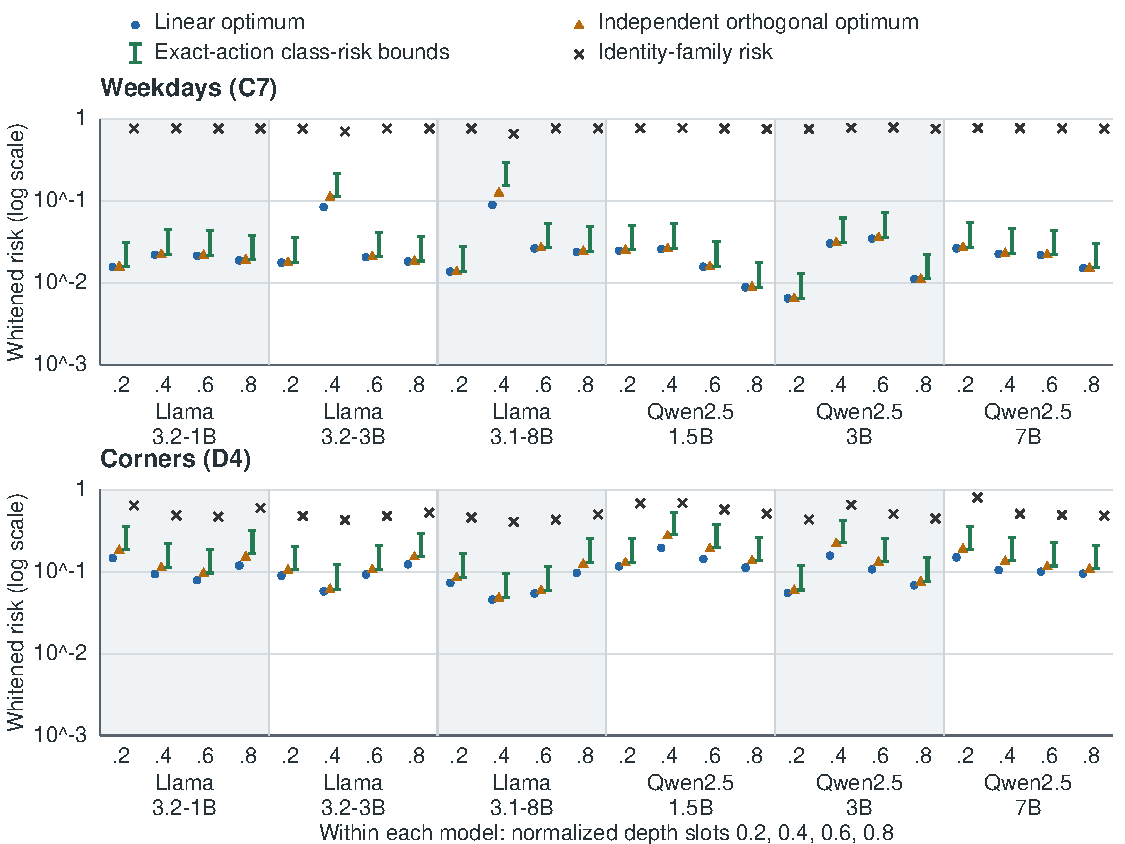
\includegraphics[width=\textwidth]{figures/same_metric_risks_v061.pdf}
\caption{\textbf{Same-metric risks in every primary condition.} Circles show $\eta$, triangles $L_{\rm orth}$, green segments $[2(1-\gamma_r),2(1-\gamma_r^2)]$, and crosses $L(I)$ at $r=16$. Within each of the 48 conditions, all four quantities use the same complete Study~2 test bank, its own second-moment whitening, and uniform state/group weights. Each model has four readouts; horizontal offsets separate symbols. The logarithmic axis shows absolute risk levels, not additive constraint costs. Segments bound the exact-action class optimum; they are neither confidence intervals nor measured witness losses. All conditions are retained. Training-metric witness transfer is reported separately in \cref{sec:witness-transfer}.}
\label{fig:same-metric-risks}
\end{figure}

\Needspace{11\baselineskip}
\paragraph{Invariant components contribute to high budgets.}
The selected trivial contributions average $b_{\rm triv}=0.61540/0.72742$ for C7/D4: much of the captured energy is invariant to the state action. These are fractions of total whitened energy, not fractions of $\gamma_r$, and need not equal the total trivial energy used by $L(I)$. Invariant components may include contextual or constant structure; state-dependent components can still encode categories. The type correction is also small in most primary conditions: the unnormalized $|\Delta_{\rm type}|$ is at most $5.33\times10^{-15}$ in 47/48. Only Llama-3.1-8B/C7/layer 13 has a material correction, with $\Delta_{\rm type}/16=0.00827$. Thus the correction to ordinary spectral truncation is concentrated at dimension 16. This correction compares the typed budget with ordinary top-$r$ truncation and does not measure the further group-law cost. A near-zero $\Delta_{\rm type}$ can coexist with a positive lower bound on $L^\star-L_{\rm orth}$. The detailed type decomposition is in \cref{app:bounded-risk-details}.

\subsection{Transfer of constructed exact actions}
\label{sec:witness-transfer}
\begin{table}[t]
\caption{Transfer of frozen predictors at $r=16$ in the training metric. These means use training whitening for both construction and old test banks, including identity and fixed points. OLS and ridge need not obey group laws. The witness is feasible, not claimed optimal. Its transfer loss is not checked against Table~\ref{tab:core-risk-summary}'s test-metric exact-orthogonal bounds: changing whitening can also change admissibility of the same raw-coordinate function.}
\label{tab:followup-witness}
\centering\small
\begin{tabular}{@{}lrrrrr@{}}
\toprule
& Construction bank & \multicolumn{3}{c}{Old test bank, frozen training metric} & Witness worse \\
Domain & Witness & Witness & OLS & Ridge & than OLS \\
\midrule
$C_7$ & 0.02906 & 0.02806 & 0.02141 & 0.02141 & 24/24 \\
$D_4$ & 0.11996 & 0.11117 & 0.08878 & 0.08878 & 24/24 \\
\bottomrule
\end{tabular}
\end{table}

The bounds concern the best member of an entire class on one bank. To evaluate an exact action as a predictor, we construct a \emph{witness}: one feasible operator family, rather than a claimed minimizer. The training bank first supplies the second-moment whitening and the type-constrained subspace selection. The construction retains complete real irreducible blocks, forms an equivariant basis, and uses orthogonal Procrustes alignment to express the resulting action in the training-whitened coordinates. For C7 this preserves complete rotation planes; for D4 it also preserves the reflection pairing of its two-dimensional type. The operators and whitening transform are then frozen for held-out evaluation.

All 48 constructions pass the specified action-law and orthogonality checks, and their construction-bank risks lie within the analytic bounds. These numerical checks verify the implemented construction at the declared tolerances; they are not interval-arithmetic certificates or evidence of class optimality.

On the held-out bank, witness losses average $0.02806/0.11117$ for C7/D4, compared with $0.02141/0.08878$ for training-fitted OLS. The witness has higher loss than OLS and fixed-coefficient ridge in every condition (Table~\ref{tab:followup-witness}). Training whitening makes the ridge baseline nearly a rescaling of the OLS matrices by $1/1.001$. Exact algebraic structure is therefore feasible here without improving this constructor's transfer performance. The ordering is empirical: class inclusion on one distribution does not force an ordering between training-fitted predictors on another.

The comparison also uses a different metric from the preceding bank bounds. Both construction and held-out witness losses retain the \emph{training} whitening, whereas Table~\ref{tab:core-risk-summary} characterizes the test bank in its \emph{own} whitening. Re-expressing the training action in test-whitened coordinates preserves its group law by conjugacy, but need not preserve orthogonality. The reported transfer losses therefore use a different metric from those intervals. Using a witness loss as a feasible-action upper bound requires evaluation under the same loss and verification that the action belongs to the corresponding exact orthogonal class. The constructor and coordinate-change derivation are given together in \cref{app:metric-conjugation}.

\subsection{Semantic registration and dimensional sensitivity}
\label{sec:registration-sensitivity}
The existence of a compatible action leaves open which candidate state-action image receives stronger spectral support. We enumerate all 120 distinct cyclic order-seven permutation-image subgroups on the weekdays and all three dihedral order-eight images on the corners, including the prescribed image. These counts concern image subgroups, not choices of generators or arbitrary inconsistent relabelings. Every candidate defines coherent transformed targets on the same source bank. Within the prescribed C7 image, the one-day, two-day and reverse generators are reparameterizations with the same full-group spectral score. The comparison therefore does not distinguish these assignments of a named generator.

On the original $r=16$ banks, the prescribed image leads all alternatives in $\gamma_r$ by more than the recorded pairwise tolerance in 7/24 C7 and 16/24 D4 conditions. To interpret these ranks, we also compare absolute score margins. For the prescribed image $H_0$, let
\[
 d_{\rm top}=\gamma_r(H_0)-\max_{H\ne H_0}\gamma_r(H),\qquad
 d_{\rm median}=\gamma_r(H_0)-\operatorname{median}_{H\ne H_0}\gamma_r(H).
\]
The median strongest-alternative margin is $-5.52\times10^{-6}$ in C7 and $5.96\times10^{-6}$ in D4 (Table~\ref{tab:bounded-margins}). C7's score spread across all images has median $3.88\times10^{-5}$ and maximum $4.07\times10^{-4}$, although the prescribed image's rank ranges from first to a numerical tie interval of 102--105 among 120. D4 spans all three ranks, with median spread $1.36\times10^{-4}$ and maximum $0.03984$. Rank changes can therefore accompany small absolute changes, particularly for weekdays. These are spectral-budget comparisons between registered tasks, not exact-$L^\star$ rankings, permutation $p$-values or semantic probabilities.

\begin{table}[t]
\caption{Registration margins in the normalized score $\gamma_r$ at $r=16$ in all 24 fixed conditions per domain. Positive margins indicate a larger score for the prescribed image than for the strongest or median alternative. U/T/B counts unique leading, tied leading and behind under the recorded pairwise tolerance. The margins compare coherent target actions.}
\label{tab:bounded-margins}
\centering\small
% Generated by analysis/main30_bounded_v1/derive.py; never edit numbers.
\begin{tabular}{llrrrc}
\toprule
Domain & Margin & Median & Min. & Max. & U/T/B \\
\midrule
C7 & $d_{\rm top}$ & $-5.52\!\times\!10^{-6}$ & $-3.03\!\times\!10^{-4}$ & $1.97\!\times\!10^{-5}$ & 7/0/17 \\
 & $d_{\rm median}$ & $1.60\!\times\!10^{-6}$ & $-4.13\!\times\!10^{-5}$ & $4.42\!\times\!10^{-5}$ &  \\
D4 & $d_{\rm top}$ & $5.96\!\times\!10^{-6}$ & $-1.23\!\times\!10^{-2}$ & $3.82\!\times\!10^{-2}$ & 16/0/8 \\
 & $d_{\rm median}$ & $1.46\!\times\!10^{-5}$ & $-2.04\!\times\!10^{-3}$ & $3.90\!\times\!10^{-2}$ &  \\
\bottomrule
\end{tabular}

\end{table}

A shared invariant component does not by itself settle this comparison. All enumerated images are transitive, so their full trivial energy $e_{\rm triv}$ is the same within a fixed bank: the invariant projection is the within-template state mean. Their selected contributions $b_{\rm triv}$ can differ because types compete for the dimension budget (\cref{sp:transitive-trivial-energy}).

A uniquely leading image still leaves its generator reparameterizations unresolved. The mechanism constructions illustrate a separate limit of exact-action compatibility. Both a shared-action construction and a stable-code construction have machine-scale noiseless witness loss, while the sampled contextual-orientation construction has smaller budgets. The stable-code construction itself supports a valid shared action. It establishes that stable coding is compatible with these diagnostics, without identifying the empirical representations with that construction or calibrating a semantic classifier (\cref{tab:followup-simulations}).

\paragraph{Sensitivity to the state-invariant component.}
We assess this dependence by subtracting the mean across states
within each complete test template in the saved 16-dimensional
Study~2 coordinates.
We compare the original observations with two centered versions,
one retaining the original test-bank whitening and the other
using the centered bank's own second-moment whitening.
For all three treatments, we rank candidate images by
$s_{16}=C_{16}/16$ and compute the strongest-alternative margin
using this score.
Table~\ref{tab:template-centering-main} reports the results.
With the original whitening retained, centering increases the
number of conditions in which the prescribed weekday image
is uniquely leading by $s_{16}$, while the prescribed corner
image falls behind an alternative in every condition.
Thus the loss of the original D4 lead already occurs under the
original whitening metric.
Rewhitening further changes the weekday leading count and the
margins in both domains.
These comparisons show that spectral preference within the
retained space depends on the inclusion of state-invariant
components and on the whitening metric.
The disappearance of a prescribed-image lead is a ranking
result and does not establish that exact actions cease to exist.
The fixed-whitening centered treatment is reported through
spectral budgets and ranks, without applying the
unit-second-moment risk bounds to its score.
The construction and numerical checks are given in
\cref{app:template-centering-sensitivity}.

\begin{table}[!htbp]
\centering
\small
\setlength{\tabcolsep}{5pt}
\caption{
Registration sensitivity to within-template centering at $r=16$.
Each domain contains 24 model--layer conditions.
The mean score refers to the prescribed image.
U/T/B counts conditions in which it is uniquely leading,
tied for the lead, or behind.
The margin is its score minus the largest alternative score,
with the median taken across conditions.
For the original and rewhitened centered treatments,
$s_{16}=\gamma_{16}$.
For centered observations retaining the original whitening,
$s_{16}$ uses the original total energy as its denominator,
rather than the remaining centered energy.
Rewhitening changes the metric.
}
\label{tab:template-centering-main}
\begin{tabular}{llrcr}
\toprule
Domain & Treatment & Mean $s_{16}$ & U/T/B
       & Median $d_{\rm top}$ \\
\midrule
$C_7$ & Original
      & 0.985102 & 7/0/17
      & $-5.52\times10^{-6}$ \\
      & Centered, original whitening
      & 0.376059 & 15/0/9
      & $+8.47\times10^{-5}$ \\
      & Centered, own whitening
      & 0.638632 & 18/0/6
      & $+8.46\times10^{-3}$ \\
\midrule
$D_4$ & Original
      & 0.935278 & 16/0/8
      & $+5.96\times10^{-6}$ \\
      & Centered, original whitening
      & 0.252296 & 0/0/24
      & $-6.76\times10^{-4}$ \\
      & Centered, own whitening
      & 0.596606 & 0/0/24
      & $-2.56\times10^{-2}$ \\
\bottomrule
\end{tabular}
\end{table}

% Format-only selection from the completed sensitivity coverage.
\begin{table}[t]
\caption{Retained-dimension sensitivity on the same complete Study~2 banks. Each row summarizes all 24 fixed conditions; $p^-$ is the lower endpoint for joint exact-law and orthogonality cost. The last column counts a uniquely highest budget for the specified semantic image among all 120 C7 or three D4 images, using the original tolerance. Eight coordinates are the leading eight saved PCA coordinates. The dimensions have different whitened metrics and normalizations; these are not optimal-dimension comparisons or significance tests.}
\label{tab:sensitivity-main}
\centering\small
\setlength{\tabcolsep}{5pt}
\begin{tabular}{@{}lrrrr@{}}
\toprule
Domain & $r$ & Mean $\gamma_r$ & Median $p^-$ & Unique leading image \\
\midrule
$C_7$ & 16 & 0.985102 & 0.000389 & 7/24 \\
$C_7$ & 8 & 0.933943 & 0.041288 & 4/24 \\
\addlinespace
$D_4$ & 16 & 0.935278 & 0.018756 & 16/24 \\
$D_4$ & 8 & 0.959581 & 0.005865 & 19/24 \\
\bottomrule
\end{tabular}
\end{table}

Retaining eight rather than sixteen coordinates changes the answer quantitatively (Table~\ref{tab:sensitivity-main}). The prescribed image is uniquely leading in 4/24 C7 and 19/24 D4 conditions, and the C7 type correction exceeds the original comparison tolerance in eight conditions rather than one. No D4 condition exceeds it at either dimension. This count applies the recorded comparison tolerance to the unnormalized $\Delta_{\rm type}$, as specified in \cref{app:spectral-dimension-sensitivity}. The absence of a consistently leading prescribed image persists, but the margins, costs and preferred images depend on the observation space. Each dimension has its own second-moment metric and $1/r$ normalization, so this is not a common-loss contest to choose an optimal dimension. The full comparison is provided in \cref{app:spectral-dimension-sensitivity}; its role is to reveal dependence on the observation space, not to tune that space for favorable results.

\subsection{Context transport under a new language construction}
\label{sec:new-context}
\begin{table}[t]
\caption{New authored contexts under matched validation selection. Losses use old-training difference energy. Negative contrasts favor difference fitting. The last column reports the 2.5th/97.5th percentiles from 2,000 paired-family bootstrap draws; it describes conditional sensitivity over 64 authored families, not calibrated population coverage. Model/readout cells and both domains remain paired in each family.}
\label{tab:followup-context}
\centering\small\setlength{\tabcolsep}{3pt}
\begin{tabular}{@{}lrrrrr@{}}
\toprule
& \multicolumn{3}{c}{Mean context-difference loss} & Difference minus & Family sensitivity \\
Panel & Identity & Coordinate fit & Difference fit & coordinate & range \\
\midrule
$C_7$ & 0.04357 & 0.05031 & 0.04448 & -0.00583 & [-0.00668, -0.00501] \\
$D_4$ & 0.16615 & 0.12273 & 0.12892 & +0.00619 & [+0.00397, +0.00841] \\
Equal-domain mean & 0.10486 & 0.08652 & 0.08670 & +0.00018 & [-0.00103, +0.00136] \\
\bottomrule
\end{tabular}
\end{table}

A separate prediction question is whether an objective that helps within one context construction also helps on new wording. For paired variants $v=0,1$ of a context family $f$, define $u_{i,f}=z_{i,f,0}-z_{i,f,1}$ and its transformed target $u_{g(i),f}$. Coordinate fitting learns a no-intercept map from $(z_{i,t},z_{g(i),t})$ and applies it to $u$. Difference fitting learns directly from $(u_{i,f},u_{g(i),f})$. Both predictors are evaluated using squared difference error divided by the same original training difference energy $E_u$. The new comparison averages changed-state losses within each nonidentity action before giving actions equal weight. Subtracting same-state representations cancels state-only components but retains context main effects, so the target is not a pure state--context interaction.

The new bank contains 64 assistant-authored paired frames per domain, or 896 weekday and 512 corner prompts per model. Both predictors are fitted on the original training families. In the new primary comparison, each predictor selects a ridge coefficient per nonidentity action using the same context-difference loss on the original validation families. Fitting and selection precede evaluation on the new bank. The earlier coordinate comparator selected a single coefficient per condition using mean coordinate validation loss across actions. The new secondary comparison changes only the coordinate arm's validation criterion to coordinate loss; the difference arm is unchanged. The coordinate arm still selects a coefficient per action, so this secondary comparison does not restore the earlier shared-coefficient rule. Its difference-minus-coordinate contrast remains negative for C7 and positive for D4. The earlier test endpoint pooled changed-state pairs, which gives D4 actions different weights from the new equal-action endpoint because actions move different numbers of corners. Thus the original and new protocols differ in wording, validation selection and, for D4, action weighting. This study evaluates predictive transport on the new contexts. The protocols are detailed in \cref{app:reproduction,app:pending-protocols}.

Difference fitting minus coordinate fitting is $-0.005833$ for C7 and $+0.006190$ for D4 on average. Difference fitting has lower loss in 20/24 weekday conditions and 8/24 corner conditions. In C7, difference fitting lowers the mean from $0.05031$ to $0.04448$, while identity has a lower mean of $0.04357$. In D4, both fitted predictors improve on identity on domain means, with coordinate fitting giving the lowest mean (Table~\ref{tab:followup-context}). With the chosen domain weights and domain-specific normalizations, the two contrasts yield an equal-domain mean of $+0.000178$, with family-resampling percentiles $[-0.001035,+0.001362]$. This resampling holds the fitted predictors and selected coefficients fixed. The domain-specific comparisons show lower loss from difference fitting for weekdays and higher loss for corners on this authored bank.

\begin{figure}[!ht]
\centering
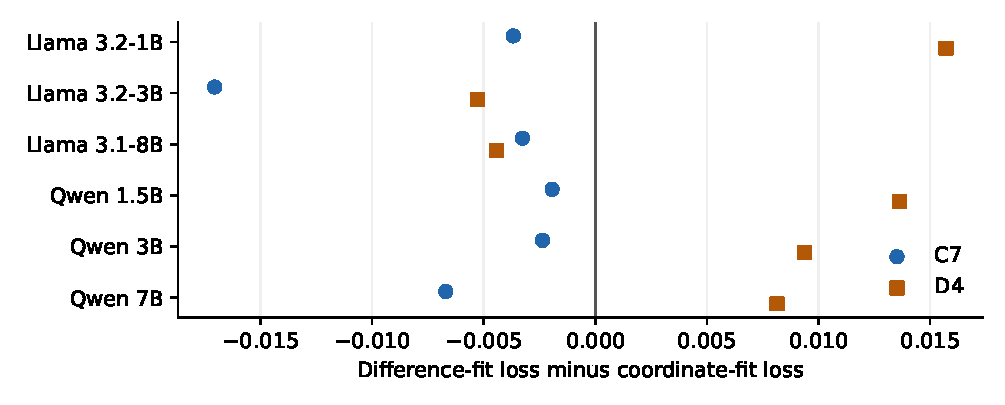
\includegraphics[width=.88\textwidth]{figures/context_transfer_followup.pdf}
\caption{New-context difference-fit minus coordinate-fit loss by model, averaged over four fixed readouts. Negative values favor difference fitting. All six weekday model means are negative, whereas four corner model means are positive. The points summarize the selected panel, not independent population draws; Table~\ref{tab:followup-context} gives the paired-family sensitivity ranges.}
\label{fig:context-followup}
\end{figure}

The frames retain the seen state vocabulary while changing outer narratives and limited factual wording. They are authored pairs, not independent human-prose samples. In a causal decoder, the state-span readout depends only on the tokenized prefix through the last selected token, as specified in \cref{sec:setup}. For D4, the difference-minus-coordinate contrast changes from $-0.015918$ under the original protocol to $+0.006190$ under the new one. The change in sign compares two protocols that vary wording, validation selection and action weighting together; it does not isolate the effect of new wording. The paired-family resampling contract is in \cref{app:pending-protocols}.

\FloatBarrier

% Keep the Discussion heading with its opening paragraph.
\Needspace{12\baselineskip}
\section{Discussion and Limitations}
\label{sec:reading-protocol}
Our evaluations distinguish held-out prediction, exact-action compatibility on a fixed bank, and spectral preference among coherent state actions.
The class-risk bounds apply to a common set of observations, targets, weights and whitening metric.
An independent orthogonal comparator gives the orthogonality cost and bounds the further cost of enforcing the group law, without requiring a fitting algorithm to attain the class optimum.
Witness transfer evaluates a separate object: a particular action constructed in training-whitened coordinates and tested with that metric frozen.
Its higher held-out loss than OLS is consistent with the class bounds, which use the test bank's own whitening and concern its best exact orthogonal action (\cref{sec:witness-transfer}).

The empirical interpretation depends on the magnitude and distribution of the computed bounds.
Positive joint-cost lower endpoints follow from a positive independent-linear optimum $\eta>0$ under the theorem's assumptions.
At $r=16$, one weekday condition contributes $99.44\%$ of the sum of the further group-law lower endpoints $\ell^-$; this is a concentration of lower bounds, not a share of the unknown true costs.
The wider upper bounds allow larger actual costs elsewhere.
Deleting individual complete C7 families preserves this concentration under each reduced bank's own whitening, but does not test alternative-image rankings (\cref{app:c7-family-influence}).
The representation-type correction measures a different quantity: the loss in captured energy relative to ordinary spectral truncation.
It exceeds the declared comparison tolerance in one primary condition and in eight C7 conditions at $r=8$.
Neither this count nor a small correction determines the additional group-law cost.

The centering diagnostic shows that registration preference depends on which components enter the dimension budget.
Across the original banks, within-template centering with the original whitening, and centering with its own whitening, the prescribed image is uniquely leading in $7$, $15$ and $18$ of the 24 weekday conditions, compared with $16$, $0$ and $0$ corner conditions (\cref{tab:template-centering-main}).
The corner image falls behind an alternative in every centered condition even before the whitening metric changes.
All candidate images are transitive and share the same total trivial-component energy within a bank; removing this component changes the competition for the finite dimension budget.
The resulting ranks compare relative spectral support and do not establish the absence of compatible exact actions.
The increase in weekday leading counts also does not imply improvement in every condition.
A stable state code remains compatible with accurate transformations, and even a uniquely leading image leaves its generator reparameterizations unresolved.

The new-context experiment addresses predictive transport separately.
Under its evaluation protocol, difference fitting lowers weekday mean loss and raises corner mean loss relative to coordinate fitting.
This is not a replication of class-risk or registration rankings.
The comparison with the earlier protocol changes wording, validation selection and, for D4, action weighting together, so the change in the D4 contrast cannot be attributed to wording alone.
The result supports a domain-dependent comparison of the two fitting objectives on the authored bank (\cref{sec:new-context}).

The retained coordinates also limit the interpretation.
Study~1 fixed $q=16$ before its final structural run, although the available records do not establish why that particular value was initially preferred.
Study~2 retained 16 for comparability with its development analyses and fitted PCA on its own training bank (\cref{app:dimension-rank-audit}).
These records establish an analysis setting, not optimality or external preregistration.
The eight-coordinate analysis supplies a sensitivity check.
Centering the saved coordinates probes the existing 16-dimensional subspace; it neither measures the fraction of full-dimensional within-template variation retained nor substitutes for PCA fitted to within-template differences.
Such a comparison would require full-dimensional readouts, a basis fitted on training differences, and a separate evaluation.

The primary representation analyses use a fixed panel of six models and four readouts per model.
These repeated measurements do not constitute independent samples from a population of language models.
The main tasks and new-context bank retain already-seen state identities.
In the joint held-out stratum of the supplementary $S_3$ task, entity names and contexts are held out while the abstract assignment states remain familiar; its predictive results do not establish native group computation.
Historical activation edits use different information and intervention spaces, and the separate native-program branch failed its clean-task competence gate, leaving its confirmation analysis blocked (\cref{app:behavior,app:reproduction}).
This limits what that protocol establishes about computation.
The finite-bank bounds likewise require additional sampling assumptions for population-level guarantees.

For other representation studies, each claim should specify the retained dimension, centering, metric, target correspondences and evaluation weights.
A held-out score evaluates a trained predictor; a class-risk interval evaluates compatibility on a fixed bank; a registration margin compares spectral budgets across coherent targets.
For centered observations retaining the original whitening, $C_{16}/16$ is normalized by the original energy and cannot be inserted directly into the unit-second-moment risk bounds.
Keeping these evaluation objects explicit allows predictive, structural and registration results to be interpreted together.

\section{Conclusion}
We derive computable bounds on the minimum prediction risk of fixed-dimensional exact orthogonal actions from a type-constrained invariant-subspace budget.
On each complete representation bank, independent linear and orthogonal comparators under the same whitened loss identify the orthogonality cost and bound the additional cost of enforcing the group law.
The computed lower bounds vary substantially across model--readout conditions.
Separately, our constructed exact actions have higher held-out loss than OLS when both are evaluated under the frozen training metric.

Spectral preference for the prescribed state-action image depends on the retained space, state-invariant components and whitening metric.
Within-template centering increases the number of conditions in which the prescribed weekday image leads, but leaves the prescribed corner image behind an alternative in every condition, even with the original whitening retained.
Rewhitening further changes the scores and rankings.
These are changes in relative spectral support.
On the separately authored context bank, difference fitting lowers mean transport loss relative to coordinate fitting for weekdays but raises it for corners.
Predictive recovery, fixed-bank compatibility with exact orthogonal actions, and spectral preference among candidate images therefore support distinct claims about the observed representations.
Establishing that the model itself uses these transformations in computation requires additional evidence.


\FloatBarrier
\label{sec:main-end}

\section*{Impact Statement}
These diagnostics concern representations of visible states in controlled language-model tasks. Presenting probe results as evidence of the model's own computation can mislead readers about its capabilities. The experiments do not assess demographic fairness or establish safety guarantees.

\bibliography{references}
\bibliographystyle{tmlr}
% Keep the complete reference list separate from the appendices.
\clearpage
\appendix
% Explicit aliases keep appendix references portable across TeX distributions.
\crefalias{section}{appendix}
\crefalias{subsection}{appendix}
\crefalias{subsubsection}{appendix}
\crefname{appendix}{Appendix}{Appendices}
\Crefname{appendix}{Appendix}{Appendices}
\section{Proofs and the Identification Problem}
\label{app:theory}
\label{sec:appendix}

\subsection{Supporting finite-state statements}

This appendix supports the prediction diagnostics in
\cref{sec:setup}, the distinction between linear and exact
orthogonal realizations in \cref{sec:boundaries}, and the
interpretation of the experiments in \cref{sec:evidence}.
We distinguish exact realizability on a finite bank,
prediction risk in specified analytical constructions,
and error identities for fitted operators.
These supporting statements are not presented as new
general representation theory.

Let a finite group $G$ act on a finite state set $S$ through
the prescribed action $\alpha:G\to\mathrm{Sym}(S)$.
Write $g(i)=\alpha(g)(i)$.
For rows indexed by state and template, define
\[
 (P_gZ)_{(i,t)}=z_{g(i),t}.
\]
Thus
\[
 P_gP_h=P_{h\circ g}.
\]
Matrices act on representation rows by right multiplication,
so an exact row action satisfies
\[
 R_gR_h=R_{h\circ g},
 \qquad R_e=\Id.
\]
The same notation applies to a single template.
The symbol $M^\dagger$ denotes the Moore--Penrose
pseudoinverse of a matrix $M$.

\begin{proposition}[Finite-orbit realizability]
\label{prop:finite}
Let $n\geq2$ and let
$X\in\R^{n\times(n-1)}$ have zero mean across rows and
rank $n-1$.
Every permutation of its rows has a unique invertible
linear realization.
In particular, for the prescribed state action,
\[
 R_g=X^\dagger P_gX
\]
is the unique matrix satisfying $XR_g=P_gX$, and
\[
 R_gR_h=R_{h\circ g}.
\]
\end{proposition}

The proof and its consequence for second-moment whitening
are given in \cref{app:finite-orbit-proof}.

For arbitrary fitted matrices, write
\[
 e_g(i,t)=z_{i,t}R_g-z_{g(i),t}.
\]

\begin{proposition}[Prediction-error propagation]
\label{prop:propagation}
For $p=g_1\circ g_2$, the composition residual satisfies
\begin{align}
 z_{i,t}(R_{g_2}R_{g_1}-R_p)
 &=e_{g_2}(i,t)R_{g_1} \nonumber\\
 &\quad+e_{g_1}(g_2(i),t)-e_p(i,t).
\end{align}
Consequently,
\begin{align*}
 &\norm{z_{i,t}(R_{g_2}R_{g_1}-R_p)}_2\\
 &\quad\leq
 \norm{e_{g_2}(i,t)}_2\norm{R_{g_1}}_{\rm op}
 +\norm{e_{g_1}(g_2(i),t)}_2
 +\norm{e_p(i,t)}_2.
\end{align*}
\end{proposition}

The proof and the conditions needed to relate this identity
to normalized diagnostics are given in
\cref{app:propagation-proof}.

\begin{proposition}[Global-field cancellation]
\label{prop:additive}
For any permutation $g$ of a complete, uniformly weighted
state set in a template,
\[
 \sum_{i\in S}(z_{g(i),t}-z_{i,t})=0.
\]
Therefore the balanced training estimator
\[
 v_g=\mathbb E_{i,t}
       [z_{g(i),t}-z_{i,t}]
\]
is zero for every group element.
\end{proposition}

The proof and its scope are given in
\cref{app:global-cancellation-proof}.


\subsection{Finite-orbit realizability}
\label{app:finite-orbit-proof}

\begin{proof}[Proof of \cref{prop:finite}]
Centering implies
$\operatorname{col}(X)\subseteq\mathbf1^\perp$.
Both spaces have dimension $n-1$, so they are equal.
Every permutation matrix preserves $\mathbf1^\perp$;
hence $P_gX$ lies in the column space of $X$.
Full column rank gives the unique solution
\[
 R_g=(X^\top X)^{-1}X^\top P_gX.
\]
Using $P_gP_h=P_{h\circ g}$,
\[
 XR_gR_h
 =P_gXR_h
 =P_gP_hX
 =P_{h\circ g}X
 =XR_{h\circ g}.
\]
Full column rank establishes the multiplication rule.
The identity permutation gives $R_e=\Id$.
Taking $h=g^{-1}$ gives both inverse identities, so every
$R_g$ is invertible.
The argument applies to every permutation of the $n$ rows.
\end{proof}

If $n$ lexical vectors are affinely independent, their
centered span has dimension $n-1$.
Retaining all these PCA dimensions gives coordinates on
that entire span, so the proposition applies.
Neither regular polygon geometry nor prior knowledge of a
named group is required.
The resulting matrices need not be orthogonal in the
original Euclidean coordinates.

For the uniform state distribution, however, define
\[
 \Sigma=\frac1nX^\top X\succ0.
\]
Exact realization and $P_g^\top P_g=\Id_n$ imply
\[
 R_g^\top\Sigma R_g
 =\frac1n(P_gX)^\top(P_gX)
 =\Sigma.
\]
In the whitened coordinates
\[
 \bar X=X\Sigma^{-1/2},
 \qquad
 Q_g=\Sigma^{1/2}R_g\Sigma^{-1/2},
\]
we therefore have
\[
 \bar XQ_g=P_g\bar X,
 \qquad
 Q_g^\top Q_g=\Id_{n-1},
 \qquad
 Q_gQ_h=Q_{h\circ g}.
\]
Thus every state permutation has an exact orthogonal
realization after whitening this full centered state span.
This is the shared-code case used in
\cref{sec:boundaries}; it does not assert that arbitrary
truncated or context-dependent coordinates have the same
property.

A related interpolation issue arises in representation
comparison: invariance to arbitrary invertible linear
changes can make sufficiently high-dimensional sample
representations indistinguishable
\citep{kornblith2019similarity}.
That result concerns comparison statistics in the relevant
sample-rank regime.
It does not establish transformation prediction in new
contexts or imply that the present 16-dimensional banks
fall into that regime.


\subsection{Separate contextual realizations need not be shared}

Consider the centered three-state coordinates
\[
 X=
 \begin{bmatrix}
  1&0\\
  0&1\\
  -1&-1
 \end{bmatrix},
 \qquad
 R=
 \begin{bmatrix}
  0&1\\
  -1&-1
 \end{bmatrix}.
\]
For the cycle $g:1\mapsto2\mapsto3\mapsto1$,
$XR=P_gX$.
A second contextual copy $Y=XA$, with
$A=\operatorname{diag}(2,1)$, has the forced operator
\[
 R'=A^{-1}RA
 =
 \begin{bmatrix}
  0&1/2\\
  -2&-1
 \end{bmatrix}
 \ne R.
\]
A shared operator $M$ would satisfy both
$XM=P_gX$ and $YM=P_gY$.
Full column rank forces $M=R$ from the first equation and
$M=R'$ from the second, a contradiction.

This example shows that separate realizability within
each context does not guarantee one realization in the
common coordinates.
The contradiction uses fully supported coordinates;
different arbitrary extensions on unobserved directions
would not suffice.
Applying one common invertible coordinate change to both
contexts, including a common whitening, preserves the
contradiction.
Realigning the contexts separately changes the shared-map
question.

Testing a training-fitted family on held-out contexts
therefore asks more than whether each individual orbit
admits some action.
Success on finitely many held-out contexts still does not
establish a shared action on an unrestricted population of
contexts.


\subsection{Shared contextual realizations can still reflect state identity}

Shared realizability does not by itself identify semantic
computation.
Let $a_i\in\R^{1\times(n-1)}$ be a centered,
full-affine-rank state code, and let
$c_t\in\R^{1\times m}$ be a context vector.
By \cref{prop:finite}, there are matrices $B_g$ satisfying
$a_iB_g=a_{g(i)}$ and the row-action law.
For
\[
 z_{i,t}=(a_i,c_t),
 \qquad
 R_g=
 \begin{bmatrix}
  B_g&0\\
  0&\Id_m
 \end{bmatrix},
\]
one shared family maps all contexts exactly and obeys all
group relations.
The same state code supports alternative permutation
actions on the labels.
The construction requires no account of how a language
model computes a weekday shift or a geometric rotation.
A global invertible coordinate change preserves the
example up to conjugacy, so visible separation of state
and context coordinates is unnecessary.

The strict additive form has a further implication.
For a fixed invertible $T$, suppose
\[
 z_{i,t}=(a_i,c_t)T.
\]
Writing $\bar z_t=n^{-1}\sum_i z_{i,t}$ and
$\bar a=n^{-1}\sum_i a_i$, within-template centering gives
\[
 z_{i,t}-\bar z_t=(a_i-\bar a,0)T.
\]
All templates then share the same centered state code,
and the pooled centered matrix has rank at most $n-1$.
A fixed linear projection cannot increase that rank.

In \cref{app:template-centering-sensitivity}, all saved
centered Study~2 banks have numerical rank 16 under the
declared rule, exceeding the bounds 6 and 3 for this exact
weekday and corner construction.
The strict additive form therefore does not give an exact
description of those saved coordinates under that rank
criterion.
This observation neither measures its quality as an
approximation nor excludes stable state-code components
coexisting with context-dependent state variation.

Historical AFS-B changes operator labels inconsistently
with the prescribed multiplication table, while AFS-C
changes correspondences across training contexts;
both can damage a stable-code predictor.
The later category predictors and coherent alternative
registration in
\cref{sec:characterization,app:reproduction}
test different competing explanations.
Their predictive performance and the spectral comparisons
in \cref{sec:registration-sensitivity} address distinct
questions.
Neither identifies the strict construction above with
the measured activations or constitutes a conditional
comparison jointly matched in prediction error, operator
norm, information and capacity.


\subsection{Shared contextual actions as a subspace test}
\label{app:contextual-realization}

Stack contextual rows into $Z\in\R^{N\times q}$, with
complete state blocks, and let $P_g$ permute states within
each template.
For equal row weights and any rank of $Z$,
\[
 \min_{R\in\R^{q\times q}}
 \norm{ZR-P_gZ}_F^2
 =
 \norm{(\Id_N-ZZ^\dagger)P_gZ}_F^2.
\]
Indeed, $ZZ^\dagger P_gZ$ is the orthogonal projection of
the target matrix onto $\operatorname{col}(Z)$.
An exact shared map exists if and only if the residual
vanishes, equivalently
\[
 P_g\operatorname{col}(Z)
 \subseteq\operatorname{col}(Z).
\]
When $Z$ has full column rank, the exact solution
$R_g=Z^\dagger P_gZ$ is unique.
Existence for every group element then forces the
row-action multiplication law.

Equivalently, let
\[
 \mathcal N=\ker(Z^\top)
\]
be the space of linear dependencies among rows.
Exact realizability is equivalent to
\[
 P_g^\top\mathcal N\subseteq\mathcal N.
\]
Necessity follows from
\[
 a^\top Z=0
 \quad\Longrightarrow\quad
 a^\top P_gZ=a^\top ZR_g=0.
\]
Conversely, this condition makes
$a^\top Z\mapsto a^\top P_gZ$ well defined on the row span.
For a whole group, the induced maps are invertible and
obey the row-action law.

This is the finite row-observation form of the
kernel-preservation criterion for a transformation to
descend through a linear encoder
\citep[Theorem~1]{sun2026transformationlaws}.
The correspondence is explicit: take the linear map
$W=Z^\top$ and the input transformation $P_g^\top$, so that
\[
 R_g^\top W=WP_g^\top.
\]
Here $W$ acts on coefficients of observed rows; it is not
the language model's nonlinear encoder.
The condition concerns the left kernel of $Z$.
Preserving only equal-row pairs, or considering the right
kernel $\ker Z$, does not give this criterion.
For example, the three distinct scalar states
$(-1,0,1)$ have no exact linear realization of their
three-cycle, because $(0,1,-1)$ is not a scalar multiple
of $(-1,0,1)$.

When $Z$ is rank deficient, only the action on its row
span is identified.
Set
\[
 H_Z=Z^\dagger Z,
 \qquad
 S_g=Z^\dagger P_gZ.
\]
The minimum-norm identity solution is $S_e=H_Z$, a
projector rather than the ambient identity.
If all the subspace conditions hold, then
\[
 H_ZS_g=S_gH_Z=S_g
\]
and
\[
 \begin{aligned}
 S_gS_h
 &=Z^\dagger P_g(ZZ^\dagger)P_hZ\\
 &=Z^\dagger P_gP_hZ
 =S_{h\circ g}.
 \end{aligned}
\]
The second equality uses
$ZZ^\dagger P_hZ=P_hZ$.
Consequently,
\[
 \widetilde R_g=S_g+(\Id_q-H_Z)
\]
acts as the induced action on the row span and as identity
on its orthogonal complement, with
\[
 \widetilde R_e=\Id_q,
 \qquad
 \widetilde R_g\widetilde R_h
 =\widetilde R_{h\circ g}.
\]
Inverses follow from the group law.
The complementary action is a choice.
The action on the observed row span is unique; the full
ambient matrix is unique only when $Z$ has full column
rank.
New contexts can impose additional constraints.

For a complete uniformly weighted bank with full column
rank, exact linear realizability also connects directly
to the whitened class in \cref{eq:class-loss-main}.
Let
\[
 \Sigma=\frac1N Z^\top Z\succ0.
\]
If $ZR_g=P_gZ$, then
\[
 R_g^\top\Sigma R_g
 =\frac1N(P_gZ)^\top(P_gZ)
 =\Sigma.
\]
Thus
\[
 \rho_g=\Sigma^{1/2}R_g\Sigma^{-1/2}
\]
is orthogonal, realizes the action on $Z\Sigma^{-1/2}$,
and preserves the row-action law.
Under this common whitened loss,
\[
 \eta=0
 \quad\Longrightarrow\quad
 L_{\rm orth}=L^\star=0.
\]
This is a zero-risk implication.
It does not identify the three optima when their risks
are positive.
A weighted version requires the weighting matrix $D$ to
satisfy $P_g^\top DP_g=D$ and
$Z^\top DZ\succ0$.
Weights that vary only across complete templates satisfy
the invariance requirement.

The projection formula above is an unregularized,
unnormalized, finite-bank characterization.
It is not the row-normalized held-out score in
\cref{eq:D}, and it gives no population guarantee.
Orthogonality in the original Euclidean coordinates or
in another specified metric requires its own check.
A rank-deficient bank also does not satisfy the
$q$-dimensional unit-second-moment condition merely
because an invertible ambient extension exists.

For comparison, the ridge objective
\[
 \norm{ZR-P_gZ}_F^2+\lambda\norm R_F^2,
 \qquad \lambda>0,
\]
returns
\[
 R_g^{(\lambda)}
 =(Z^\top Z+\lambda\Id_q)^{-1}Z^\top P_gZ.
\]
Here $\lambda$ is the penalty in this unnormalized
objective; a coefficient specified in an
energy-normalized implementation must first be converted
to this convention.
If an exact $R_g^\star$ exists, then
\[
 R_g^{(\lambda)}=B_\lambda R_g^\star,
 \qquad
 B_\lambda
 =(Z^\top Z+\lambda\Id_q)^{-1}Z^\top Z.
\]
In particular, the independently fitted identity is
$B_\lambda$, which generally differs from $\Id_q$.
Shrinkage can introduce power and relation errors even
in an exactly realizable system.
The relation and identity penalties in Joint address
these departures, but their empirical effects do not
by themselves isolate additional semantic information.


\subsection{An exact common-design ridge identity}
\label{app:ridge-identity}

Suppose every element uses the same source matrix
$Z\in\R^{N\times q}$, the same effective penalty
$\lambda>0$, and targets $P_gZ$ from one coherent group
action.
Define
\begin{align*}
 L_\lambda
 &=(Z^\top Z+\lambda\Id_q)^{-1}Z^\top,\\
 \mathsf E_\lambda
 &=\Id_N-ZL_\lambda,
 \qquad
 R_g=L_\lambda P_gZ.
\end{align*}
The symbol $\mathsf E_\lambda$ denotes the ridge residual
operator, not an orbit-Gram matrix.

Using $P_gP_h=P_{h\circ g}$ gives
\begin{align}
 ZR_g-P_gZ
 &=-\mathsf E_\lambda P_gZ,
 \label{eq:ridge-fit-identity}\\
 R_gR_h-R_{h\circ g}
 &=-L_\lambda P_g\mathsf E_\lambda P_hZ.
 \label{eq:ridge-law-identity}
\end{align}
For the first identity, substitute
$ZL_\lambda=\Id_N-\mathsf E_\lambda$ into $ZR_g$.
For the second,
\[
 \begin{aligned}
 R_gR_h
 &=L_\lambda P_g(ZL_\lambda)P_hZ\\
 &=L_\lambda P_gP_hZ
   -L_\lambda P_g\mathsf E_\lambda P_hZ.
 \end{aligned}
\]
No exact realizability or full-rank assumption is needed.
For $\lambda>0$, $\mathsf E_\lambda$ is generally not
an orthogonal projector.

Coherence of the target action is essential to the
second identity.
If instead the targets use arbitrary permutation matrices
$\widetilde P_g$, with
$\widetilde R_g=L_\lambda\widetilde P_gZ$, then
\[
 \begin{aligned}
 \widetilde R_g\widetilde R_h
 -\widetilde R_{h\circ g}
 &=-L_\lambda\widetilde P_g
      \mathsf E_\lambda\widetilde P_hZ\\
 &\quad+
 L_\lambda
 \bigl(\widetilde P_g\widetilde P_h
       -\widetilde P_{h\circ g}\bigr)Z.
 \end{aligned}
\]
The extra term prevents applying
\cref{eq:ridge-law-identity} unchanged to inconsistent
operator relabelings or target scrambling.

The common-design identities apply directly to the full
independent Ridge fit in Study~1.
They do not apply unchanged to Joint after optimization,
to a family formed by composing fitted generators, or
to fits with element-specific source subsets, weights,
penalties or independently centered targets.
They explain an algebraic dependence between fit and
composition defects; they are not independent
significance tests.
Their unnormalized matrix residuals must also be
distinguished from the row-normalized test metric in
\cref{eq:D}.


\subsection{Equal within-context geometry need not permit shared transport}
\label{app:orientation}

We give a restricted analytical construction using
orthogonal representations and group averaging
\citep{serre1977linear}.
It specifies an identification boundary, rather than
a model assumed for the measured activations.

Let $1\leq k\leq n-1$ and let
$V\in\R^{n\times k}$ satisfy
\[
 \mathbf1^\top V=0,
 \qquad
 V^\top V/n=\Id_k,
 \qquad
 VQ_g=P_gV,
\]
where $Q_g\in O(k)$ and
$Q_gQ_h=Q_{h\circ g}$.
For $d\geq k$, choose
$A_c\in\R^{d\times k}$ with
$A_c^\top A_c=\Id_k$, and set
\[
 X_c=VA_c^\top.
\]
The frames belong to the Stiefel manifold
\[
 \mathrm{St}(d,k)
 =\{A\in\R^{d\times k}:A^\top A=\Id_k\}
\]
\citep{edelman1998geometry}.
This is a space of frame matrices in the construction,
not an assumed manifold of language-model activations.
Here $k$ is the intrinsic orbit rank and $d$ is the
ambient observation dimension.

Every context has the same within-context Gram matrix,
\[
 X_cX_c^\top=VV^\top,
\]
and an exact local orthogonal action
\[
 R_{c,g}
 =A_cQ_gA_c^\top+(\Id_d-A_cA_c^\top).
\]
Indeed,
\[
 X_cR_{c,g}=P_gX_c,
\]
and the two orthogonal subspaces carry $Q_g$ and the
identity, respectively.
The construction does not fix cross-context inner
products.

\begin{proposition}[Independent-orientation risk]
\label{prop:orientation}
For a nonempty $\mathcal A\subseteq G$, define
\[
 \ell_c(R)
 =\frac{1}{nk|\mathcal A|}
   \sum_{g\in\mathcal A}
   \norm{X_cR_g-P_gX_c}_F^2.
\]
Suppose a fresh $A_c$ has the uniform Stiefel distribution
induced by Haar measure on $O(d)$ and is independent of
the fitted matrices $\widehat R_g\in\R^{d\times d}$.
Then
\begin{equation}
\begin{aligned}
 &\mathbb E[\ell_c(\widehat R)\mid\widehat R]\\
 &\quad=
 b_{\mathcal A}
 +\frac{1}{d|\mathcal A|}
  \sum_{g\in\mathcal A}
  \norm{\widehat R_g-\frac{\chi(g)}k\Id_d}_F^2,
\end{aligned}
\end{equation}
where
\[
 \chi(g)=\operatorname{tr}(Q_g),
 \qquad
 b_{\mathcal A}
 =1-\frac1{|\mathcal A|}
       \sum_{g\in\mathcal A}
       \left(\frac{\chi(g)}k\right)^2.
\]
Thus $b_{\mathcal A}$ is the minimum expected risk among
unrestricted shared matrix predictors in this
construction.
\end{proposition}

\begin{proof}
Using $V^\top V=n\Id_k$,
\[
 \frac{\norm{X_cR-P_gX_c}_F^2}{nk}
 =
 \frac{\norm{A_c^\top R-Q_gA_c^\top}_F^2}{k}.
\]
Orthogonal invariance and traces give
\[
 \mathbb E[AA^\top]=\frac{k}{d}\Id_d,
 \qquad
 \mathbb E[AQ_gA^\top]=\frac{\chi(g)}d\Id_d.
\]
Expanding the square and taking expectations yields
\begin{align*}
 &\frac1d\norm R_F^2+1
   -\frac{2\chi(g)}{kd}\operatorname{tr}R\\
 &\quad=
 1-\frac{\chi(g)^2}{k^2}
 +\frac1d
  \norm{R-\frac{\chi(g)}k\Id_d}_F^2.
\end{align*}
Averaging over $\mathcal A$ proves the identity.
Independence permits conditioning on the fitted family.
The scalar matrices
$R_g=\chi(g)\Id_d/k$ attain the minimum, although they
need not form a group representation.
\end{proof}

The baseline $b_{\mathcal A}$ is an unconstrained
population prediction risk.
It is distinct from the orthogonality cost
$\beta=L_{\rm orth}-\eta$ in the main text.

For the full centered permutation representation of the
seven-state cycle,
\[
 k=6,\qquad
 \chi(e)=6,\qquad
 \chi(g)=-1\quad(g\ne e).
\]
Hence
\[
 b_G=\frac56,
 \qquad
 b_{G\setminus\{e\}}=\frac{35}{36}.
\]
For the full centered four-corner permutation
representation of $D_4$, $k=3$, and every nonidentity
character is $+1$ or $-1$, giving
\[
 b_G=\frac79,
 \qquad
 b_{G\setminus\{e\}}=\frac89.
\]
These calculations use the complete centered permutation
representations, not two-dimensional polygon coordinates.

The normalization above uses the orbit energy $nk$.
For one context,
\[
 \frac1nX_c^\top X_c=A_cA_c^\top,
\]
which has rank $k$ and is singular when $d>k$.
Under the specified Haar distribution,
\[
 \mathbb E_c\!\left[\frac1nX_c^\top X_c\right]
 =\frac{k}{d}\Id_d,
\]
but a finite context bank need not have this second
moment or even full ambient rank.
The constants therefore do not directly provide bounds
for an empirical bank whitened by its own second moment.

The full orthogonal-invariance assumption is essential.
Independence alone, or a distribution restricted to a
commuting family of rotations, is insufficient.
The constants also cannot be compared numerically with
the reported $\Eeq$, which uses a different distribution
and normalization.
No Haar randomization test or empirical rejection of
this construction is claimed.


\subsection{A commutant criterion in the full-rank construction}
\label{app:commutant}

Specialize the preceding construction to $d=k$, writing
$A_c=O_c\in O(k)$.
The orientations may now have any distribution.
Define
\begin{align*}
 \mathcal C_Q
 &=\{B\in\R^{k\times k}:BQ_g=Q_gB
                         \text{ for every }g\in G\},\\
 \Pi_Q(B)
 &=\frac1{|G|}\sum_{g\in G}Q_gBQ_g^\top.
\end{align*}
The group average is the Frobenius orthogonal projection
onto $\mathcal C_Q$.
Reindexing shows that its image commutes with every
$Q_g$; it fixes every commuting matrix; and inverse
closure makes it self-adjoint.

\begin{proposition}[Relative-orientation obstruction]
\label{prop:commutant}
Let $c,c'$ be independent draws from the context
distribution, set $U=O_c^\top O_{c'}$, and use
$\mathcal A=G$ in $\ell_c$.
Then
\[
 \inf_{\substack{R_g\in\R^{k\times k}\\g\in G}}
 \mathbb E_c\ell_c(R)
 =
 \frac1k
 \mathbb E_{c,c'}
 \norm{U-\Pi_Q(U)}_F^2.
\]
An exact shared action exists almost surely if and only
if the relative orientations commute with every $Q_g$
almost surely.
\end{proposition}

\begin{proof}
The local action is
\[
 R_{c,g}=O_cQ_gO_c^\top.
\]
Since $X_c^\top X_c/n=\Id_k$, the loss for element $g$
equals
\[
 \frac1k\norm{R_g-R_{c,g}}_F^2.
\]
Its unrestricted minimizer is
$\mathbb E_cR_{c,g}$.
The pairwise variance identity therefore gives the
optimum risk as
\[
 \frac1{2k|G|}
 \mathbb E_{c,c'}
 \sum_{g\in G}\norm{Q_gU-UQ_g}_F^2.
\]
Expansion and the projection identity yield
\[
 \frac1{|G|}
 \sum_{g\in G}\norm{Q_gU-UQ_g}_F^2
 =
 2\norm{U-\Pi_Q(U)}_F^2.
\]
This proves the risk formula.
Nonnegativity gives the zero-risk equivalence.
At zero risk, the common matrices agree almost surely
with the local orthogonal actions and inherit their
group law.
At positive risk, their means need not be orthogonal
or form a representation.
\end{proof}

Large context rotations within the commutant can leave
the action unchanged.
The proposition is a characterization of this
full-rank, whitened, noiseless construction.
Its infimum is over unrestricted shared matrices,
rather than the exact-action class defining $L^\star$.

There is also a deterministic finite-bank version.
For any fixed $m\geq1$ contexts, define
\[
 \widehat R_{m,g}
 =\frac1m\sum_{j=1}^mR_{c_j,g},
 \qquad
 \widehat L_m
 =\frac1m\sum_{j=1}^m\ell_{c_j}(\widehat R_m).
\]
The sample mean minimizes the unrestricted bank loss.
Writing $U_{ij}=O_{c_i}^\top O_{c_j}$, the same pairwise
variance identity gives
\[
 \widehat L_m
 =
 \frac1{km^2}
 \sum_{i=1}^m\sum_{j=1}^m
 \norm{U_{ij}-\Pi_Q(U_{ij})}_F^2.
\]
The sums include all ordered pairs.
No independence assumption is needed for this fixed-bank
identity.
Because every context has unit second moment, this is
the independent-linear optimum $\eta$ for the same
uniformly weighted bank and full-group loss.
It does not determine $L^\star$ when the risk is positive,
and zero bank risk alone gives no guarantee for new
contexts.

For iid training contexts, let
\[
 b=
 \inf_{\substack{R_g\in\R^{k\times k}\\g\in G}}
 \mathbb E_c\ell_c(R).
\]
If $c_{\rm new}$ is an independent draw from the same
distribution, the variance identity gives
\[
 \mathbb E\widehat L_m=(1-1/m)b,
 \qquad
 \mathbb E\ell_{c_{\rm new}}(\widehat R_m)
 =(1+1/m)b.
\]
Both expectations include the sampled training contexts;
the second also includes the fresh context.
These sample-mean identities are analytical consequences
of this construction, not learning-curve predictions
for ridge fitted to the actual 16-dimensional activations.


\subsection{Prediction-error propagation}
\label{app:propagation-proof}

\begin{proof}[Proof of \cref{prop:propagation}]
Insert and subtract
$z_{g_2(i),t}R_{g_1}$ and
$z_{g_1(g_2(i)),t}$.
Since $p(i)=g_1(g_2(i))$,
\begin{align*}
 z_{i,t}R_{g_2}R_{g_1}-z_{i,t}R_p
 &=\bigl(z_{i,t}R_{g_2}-z_{g_2(i),t}\bigr)R_{g_1}\\
 &\quad+
 \bigl(z_{g_2(i),t}R_{g_1}-z_{p(i),t}\bigr)\\
 &\quad-
 \bigl(z_{i,t}R_p-z_{p(i),t}\bigr).
\end{align*}
This is the stated identity.
The triangle inequality and
$\norm{vA}_2\leq\norm v_2\norm A_{\rm op}$
give the norm bound.
\end{proof}

For example, suppose every unnormalized prediction error
is at most $\delta$ on complete, group-closed evaluation
state blocks, and
$\norm{R_g}_{\rm op}\leq M$ for every relevant element.
Then every pairwise residual is at most
$(M+2)\delta$.
If the comparison denominators also satisfy
\[
 \norm{z_{i,t}R_p}_2^2+10^{-12}
 \geq b_{\min}>0,
\]
each corresponding normalized defect is at most
\[
 \frac{(M+2)^2\delta^2}{b_{\min}}.
\]

The uniform error assumption must cover all elements
used in the identity, including the fitted $R_e$ when
$p=e$.
The prediction aggregate $\Eeq$ excludes the identity,
whereas the products in the consistency diagnostics can
equal it.
Moreover, the consistency denominator comes from
$z_{i,t}R_p$, the directly fitted prediction, rather
than the true target $z_{p(i),t}$.

A small average prediction error supplies neither a
uniform $\delta$ nor a useful denominator lower bound.
Changed-state-only aggregates likewise do not provide
uniform control over a complete group-closed set.
The identity therefore does not yield a numerical bound
on the reported $D$ without accounting for its
sample-specific denominators and operator norms.
It explains a dependence that matters when assessing
algebraic consistency beyond predictive accuracy.
The present experiments do not include an error-matched
conditional null analysis.


\subsection{Global additive cancellation}
\label{app:global-cancellation-proof}

\begin{proof}[Proof of \cref{prop:additive}]
Since $g$ is a bijection of $S$,
\[
 \sum_{i\in S}z_{g(i),t}
 =
 \sum_{i\in S}z_{i,t}.
\]
Subtracting gives zero separately in every template.
Averaging over any common distribution of training
templates preserves zero.
\end{proof}

The cancellation holds in every representation dimension
and does not require centering or PCA.
It concerns the sum of transformation displacements:
\[
 \sum_i(z_{g(i),t}-z_{i,t})=0.
\]
It does not assert that the template mean
$n^{-1}\sum_i z_{i,t}$ is zero.
Thus it does not imply removal of the state-invariant
component studied in
\cref{app:template-centering-sensitivity}.
A numerical implementation can retain roundoff residuals.

More generally, cancellation holds for weights invariant
under the relevant permutation.
For a fixed $g$, deleting fixed-point pairs also preserves
cancellation whenever moved states remain, because each
deleted displacement is zero.
Incomplete state sets that are not preserved by $g$, or
non-invariant weights, need not cancel.
Those conditions differ from the complete balanced
training estimator considered here.

A source-state-conditioned vector,
\[
 v_{g,i}
 =\mathbb E_t[h_{g(i),t}-h_{i,t}],
\]
need not vanish because it does not average over source
states.


\subsection{State-conditioned additive actions can compose}
\label{app:additive-composition}

For training-only state means
\[
 \mu_i
 =\mathbb E_{t\in\mathcal T_{\mathrm{train}}}h_{i,t},
\]
using the same template weights for every state, the
source-conditioned comparator satisfies
\[
 v_{g,i}
 =\mathbb E_t(h_{g(i),t}-h_{i,t})
 =\mu_{g(i)}-\mu_i.
\]
To compose the edits, retain the state index and update
it after each action.
Define the augmented-state function
\[
 \mathcal A_g(h,i)
 =
 \bigl(h+\mu_{g(i)}-\mu_i,\ g(i)\bigr).
\]
For $p=g_1\circ g_2$,
\begin{align*}
 (\mathcal A_{g_1}\circ\mathcal A_{g_2})(h,i)
 &=
 \bigl(
 h+(\mu_{g_2(i)}-\mu_i)
   +(\mu_{p(i)}-\mu_{g_2(i)}),
 p(i)
 \bigr)\\
 &=
 \bigl(h+\mu_{p(i)}-\mu_i,p(i)\bigr)\\
 &=\mathcal A_p(h,i).
\end{align*}
The means telescope, and
$\mathcal A_e(h,i)=(h,i)$.
This is an exact action on the augmented space.
For noncommuting actions, the two orders can have
different target means, so the construction can preserve
order as well as composition.

The state index is part of the construction.
Without that index, this argument does not define a
linear operator family on the original hidden space.
The historical behavioral experiment supplies the source
identity as oracle information and fits displacement
vectors in the full hidden dimension.
It therefore differs from a structural comparison in
the same PCA coordinates with matched identity
information.
The coordinate-level category controls in
\cref{sec:characterization,app:reproduction} retain their
own stated information conditions.
None of these constructions identifies a native neural
mechanism.

The exact composition guarantee also differs from
re-decoding every intermediate vector.
For nearest-centroid decoding $\widehat i(h)$, define
the stateless rule
\[
 F_g(h)
 =
 h+\mu_{g(\widehat i(h))}-\mu_{\widehat i(h)}.
\]
With $\mu_0=0$, $\mu_1=2$ and the swap $s$,
\[
 F_s(-2)=0,\qquad F_s(0)=2.
\]
Thus
\[
 F_s(F_s(-2))=2\ne-2,
\]
although $s^2=e$.
Perfect decoding on clean evaluation inputs does not
certify decoding after edits.
Likewise, looking up a known composite action after one
input decode does not test repeated learned primitive
edits.

Global additive cancellation consequently does not
establish an intrinsic advantage of multiplicative
notation.
Every linear predictor can also be written as a
state-dependent displacement:
\[
 zR_g=z+z(R_g-\Id).
\]


\subsection{Faithful actions need not be free}
\label{app:faithful-not-free}

An action is faithful if no nonidentity group element
fixes every state.
It is free if no nonidentity element fixes any state.
The four-corner $D_4$ action is faithful but not free:
each corner has a stabilizer of size two.
A fixed source corner therefore has four possible
endpoints for eight group elements.

The complete labeled state correspondence distinguishes
the elements of this faithful action.
An individual source--target pair does not.
This statement concerns state labels; hidden
representations that merge states need not preserve
that distinction.
Faithfulness of the prescribed input action also does
not restrict the class in \cref{eq:class-loss-main} to
faithful representation maps.

Number the corners clockwise as
\[
 0=\mathrm{NW},\qquad
 1=\mathrm{NE},\qquad
 2=\mathrm{SE},\qquad
 3=\mathrm{SW}.
\]
Then the generators in \cref{sec:setup} are
\[
 r(i)=i+1,\qquad s(i)=1-i
 \pmod 4.
\]
Words here denote composition of input functions, with
the rightmost function applied first.
Their corresponding row-matrix products have the
reversed order.
We have
\[
 srs(i)=i-1,\qquad rsr(i)=1-i,
\]
which agree at $i=1,3$, whereas
\[
 rs(i)=2-i,\qquad sr(i)=-i
\]
differ at every corner.
Order comparisons must therefore report which source
states distinguish the tested endpoints.
Success on this four-state action does not establish
a free eight-state action or native group multiplication.


\subsection{Coordinate equivalence and the metric of approximation}
\label{app:coordinates}

For an invertible coordinate change $T_{\mathrm{coord}}$,
set
\[
 z'=zT_{\mathrm{coord}},
 \qquad
 R'_g=T_{\mathrm{coord}}^{-1}R_gT_{\mathrm{coord}}.
\]
For $p=g_1\circ g_2$,
\[
 \begin{aligned}
 z'R'_g-z'_g
 &=(zR_g-z_g)T_{\mathrm{coord}},\\
 R'_{g_2}R'_{g_1}-R'_p
 &=
 T_{\mathrm{coord}}^{-1}
 (R_{g_2}R_{g_1}-R_p)
 T_{\mathrm{coord}}.
 \end{aligned}
\]
Exact realization and exact group identities are
therefore invariant under simultaneous conjugacy.
An orthogonal coordinate change also preserves the
Euclidean row norms and Frobenius norms used in the
recorded defects.
With Euclidean scoring in both coordinate systems, a
general invertible change can alter approximate errors
and the weighting of directions.
Euclidean ridge penalties are likewise coordinate
dependent, so refitting need not return the conjugated
original estimate.

A different conclusion applies when the same full-rank
bank is reparameterized and then whitened by its own
second moment.
Let
\[
 \Sigma=\mathbb E[z^\top z]\succ0,
 \qquad
 z'=zT,
 \qquad
 \Sigma'=T^\top\Sigma T.
\]
Define
\[
 x=z\Sigma^{-1/2},
 \qquad
 x'=zT(\Sigma')^{-1/2},
 \qquad
 O_T=\Sigma^{1/2}T(\Sigma')^{-1/2}.
\]
Then
\[
 O_T^\top O_T=\Id,
 \qquad
 x'=xO_T.
\]
The two whitened banks differ only by an orthogonal
coordinate change.
Conjugating a family by $O_T$ preserves its loss,
orthogonality and group law.
Consequently, with the same observations, state
correspondences and weights, the corresponding
$\eta$, $L_{\rm orth}$, $L^\star$ and type-constrained
spectral budgets are unchanged.
Candidate-image rankings are unchanged as well.

This invariance does not identify the three treatments
in \cref{app:template-centering-sensitivity}.
Within-template centering changes the observations,
and changing the retained PCA subspace is not an
invertible change of coordinates on the same space.
Moreover, centered observations retaining the original
whitening generally do not have unit second moment.
Their score $C_{16}/16$ uses the original energy scale;
the invariance between two self-whitened descriptions
does not equate that score with the rewhitened one.

The prescribed group action on input states is also
distinct from a coordinate-equivalence group acting on
the representation description
\citep{yao2026groupaction}.
Context-specific realignments change the shared-map
question.
Changing the state correspondence while keeping the
representations fixed defines another registered task.
These operations must be distinguished when interpreting
semantic preference.

For an unnormalized activation-conditioned matrix
defect $F$,
\[
 \mathbb E\norm{zF}_2^2
 =
 \operatorname{tr}(F^\top\Sigma F),
 \qquad
 \Sigma=\mathbb E[z^\top z].
\]
Here $\Sigma$ is the uncentered second moment.
The identity shows how observation energy weights
directions.
A small data-space defect can reflect low energy in a
direction even when that direction is not exactly
unsupported.
The actual $D(A,B)$ additionally normalizes each row by
its comparison-target energy.
The operator diagnostics use different powers and, for
the C7 relation diagnostic, different aggregands.
Their numerical comparison therefore does not by itself
establish a sharp supported/unsupported distinction.

For any exact finite group action by invertible matrices,
a positive-definite invariant row metric exists.
Specifically,
\[
 H=\frac1{|G|}\sum_{g\in G}R_gR_g^\top
\]
is positive definite and satisfies
\[
 R_hHR_h^\top=H.
\]
The equality follows because multiplication by $R_h$
permutes the group-indexed family.
Choose $T_{\mathrm{coord}}$ with
$T_{\mathrm{coord}}T_{\mathrm{coord}}^\top=H$.
Then
\[
 \begin{aligned}
 R'_g(R'_g)^\top
 &=
 T_{\mathrm{coord}}^{-1}
 R_gHR_g^\top
 T_{\mathrm{coord}}^{-\top}\\
 &=\Id.
 \end{aligned}
\]
This construction chooses a metric for the given exact
action.
It does not make the original Euclidean metric invariant
or preserve a comparison that has already fixed a
different metric.
The complete-bank zero-risk argument in
\cref{app:contextual-realization} separately explains
when the bank's own whitening supplies an orthogonal
realization.
Approximately consistent fitted matrices need not
satisfy the invariant-metric identity above.

Finally, character references must match the represented
space.
The $(n-1)$-dimensional centered permutation
representation of \cref{prop:finite} has character
\[
 \chi(g)=\#\{i\in S:g(i)=i\}-1,
\]
whereas the full permutation representation has
character equal to the number of fixed states.
Additional state-invariant coordinates contribute
additional trivial characters.
Centering by the overall training mean does not
automatically remove the state-invariant variation
across templates.

These formulas therefore do not prescribe the character
of an arbitrary centered 16-dimensional representation.
Comparing normalized traces with a fixed-state-count
reference does not measure distance to every valid
representation.
Character-inner-product expressions computed from
approximately consistent fitted matrices remain
descriptive real numbers; they are not certified
integer irreducible multiplicities.

\section{Fixed-Dimensional Risk Bounds for Exact Orthogonal Actions}
\label{app:spectral-risk}

This appendix proves bounds on the minimum prediction risk over exact orthogonal actions in a fixed real dimension. The observations, target correspondences and loss are held fixed within each class comparison. Orthogonality is defined after whitening by the observation distribution's own second moment. The same analysis applies to a fixed complete bank through its empirical distribution; a population interpretation requires additional sampling assumptions. The resulting class bounds are distinct from the errors of selected fitted predictors.

\subsection{Observation contract and invariant-subspace budget}
\label{sp:setup}
Let a finite group $G$, of order $|G|$, act on a finite state set $S$, of size $n=|S|$. The state action may be nonfree or nonfaithful. A context $c$ supplies the complete labeled block $\{z_{c,s}:s\in S\}$ in fixed coordinates $z_{c,s}\in\R^{1\times r}$, with $r\ge1$. Here $(c,s)$ denotes the template--state pair written as $(t,i)$ in \cref{sec:setup}; transforming the input changes $s$ to $g\cdot s$ and leaves $c$ fixed.

Expectations use $C\sim P_C$ and an independent uniform $s\in S$. The distribution $P_C$ may be a population distribution or the declared empirical distribution of a fixed bank. Group averages include every element, including the identity, and pairs with $g\cdot s=s$ are retained. Assume finite second moments and
\[
 \Sigma=\mathbb E[z_{C,s}^{\top}z_{C,s}]\succ0,
 \qquad x=z\Sigma^{-1/2},
 \qquad \mathbb E[x^{\top}x]=\Id_r.
\]
This is second-moment whitening; zero mean is not required. The group product $gh$ means first $h$, then $g$, giving the row-action convention
\[
 \mathcal R_r(G)=\{\rho:G\to O(r):\rho_e=\Id_r,\ \rho_g\rho_h=\rho_{hg}\}.
\]
The candidate representation need not be faithful; in particular, the identity family is admissible. With $x_g(c,s)=x(c,g\cdot s)$, define two risks for the same distribution and loss:
\begin{equation}
 \begin{aligned}
 \eta
 &=
 \inf_{\{A_g\}}
 \frac1{r|G|}
 \sum_g
 \mathbb E\norm{xA_g-x_g}_2^2,
 \\
 L^\star
 &=
 \inf_{\rho\in\mathcal R_r(G)}L(\rho),
 \qquad
 L(\rho)
 =
 \frac1{r|G|}
 \sum_g
 \mathbb E\norm{x\rho_g-x_g}_2^2.
 \end{aligned}
 \label{sp:risks}
\end{equation}
The first class allows independent unconstrained $A_g\in\R^{r\times r}$; the second requires one exact $r$-dimensional orthogonal action shared across contexts. In raw coordinates $R_g=\Sigma^{-1/2}\rho_g\Sigma^{1/2}$, its loss is
\[
 \frac1{r|G|}\sum_g\mathbb E\norm{(zR_g-z_g)\Sigma^{-1/2}}_2^2.
\]
This loss differs from the row-normalized discrepancy $D$ in \cref{eq:D}, the training-energy-normalized prediction losses $E_z$ and $E_u$, and the held-out witness score computed with frozen training whitening (\cref{tab:metric-contract,sec:witness-transfer}). Under complete uniform state averaging and full-rank second moments, zero-error shared linear maps satisfy $R_g^\top\Sigma R_g=\Sigma$ and become an exact orthogonal action after whitening; \cref{app:contextual-realization} gives the realization argument. Positive-error optima over unrestricted linear maps need not have this property. Thus the bounds below concern the exact class and loss in \cref{sp:risks}. Independently fitted Ridge and finite-step penalized Joint generally do not belong to that class, and their recorded prediction scores are not feasible-action upper bounds or quantities to which its lower bound directly applies.

On the real Hilbert space $\mathcal H=L^2(P_C\times\mathrm{Unif}(S))$, define
\[
 \begin{aligned}
 (Ja)(c,s)&=x_{c,s}a,
 &
 (U_gf)(c,s)&=f(c,g\cdot s),
 \\
 P&=JJ^*,
 &
 T&=\frac1{|G|}\sum_gU_gPU_g^*.
 \end{aligned}
\]
Then $J^*J=\Id_r$, $P$ is a rank-$r$ orthogonal projection, and $U_gU_h=U_{hg}$ with each $U_g$ orthogonal. The group average $T$ commutes with every $U_g$, satisfies $0\preceq T\preceq\Id$ and $\operatorname{tr}T=r$, and is supported on
\[
 \mathcal W=\operatorname{span}\{U_gJa:g\in G,\ a\in\R^r\},\qquad \dim\mathcal W\le r|G|.
\]
Define
\begin{equation}
 \begin{aligned}
 C_r(T)&=\max_Q\operatorname{tr}(TQ),
 &
 \gamma_r&=C_r(T)/r,
 \\
 Q^2&=Q=Q^*,
 &
 [Q,U_g]&=0\quad\text{for all }g,
 \\
 \operatorname{rank}Q&\le r,
 &
 \operatorname{range}Q&\subseteq\mathcal W.
 \end{aligned}
 \label{sp:budget}
\end{equation}
The inequality $\operatorname{rank}Q\le r$ permits unused dimensions when no complete irreducible block fits the remaining budget. Thus $0\le\gamma_r\le1$. Since invariant $Q$ satisfies $\operatorname{tr}(PQ)=\operatorname{tr}(TQ)$,
\[
 r-C_r(T)=\min_Q\norm{(\Id-Q)J}_{\mathrm{HS}}^2.
\]
This is a best invariant-subspace approximation quantity, not a new notion of identifiability. Spectral constructions for invariant approximation have precedents \citep{barbieri2020approximation}; the connection to the exact-action risk is established below.

Decompose the finite-dimensional invariant space $\mathcal W$ into \emph{real} irreducible types. Let $V_\tau$ have real dimension $d_\tau$, and let $m_\tau$ be its multiplicity in $\mathcal W$. The multiplicity space has dimension $m_\tau$ over the division algebra
\[
 \mathbb D_\tau
 =
 \operatorname{End}_G(V_\tau)
 \in\{\mathbb R,\mathbb C,\mathbb H\}.
\]
The self-adjoint multiplicity operator has real eigenvalues
\[
 \lambda_{\tau,1}
 \ge\cdots\ge
 \lambda_{\tau,m_\tau}
 \ge0,
\]
counted over $\mathbb D_\tau$. Each contributes $d_\tau\lambda_{\tau,j}$ to the real trace and costs $d_\tau$ real dimensions. Thus the real dimension $d_\tau$ already accounts for complex or quaternionic type. Standard real representation theory \citep{serre1977linear} gives
\begin{equation}
 C_r(T)=\max_{\substack{k_\tau\in\{0,\ldots,m_\tau\}\\\sum_\tau d_\tau k_\tau\le r}}
 \sum_\tau d_\tau\sum_{j=1}^{k_\tau}\lambda_{\tau,j}.
 \label{sp:integer}
\end{equation}
Indeed, the commutant on each multiplicity space is a real, complex or quaternionic matrix algebra. Its self-adjoint operator diagonalizes, and the variational principle selects the largest $k_\tau$ eigenvalues for a fixed multiplicity budget. Optimizing the resulting integer real-dimension budget proves \cref{sp:integer}. A nontrivial real $C_7$ rotation plane cannot be split into two separately admissible one-dimensional directions.

\begin{spectrallemma}[Unconstrained regression risk]
\label{sp:regression}
The optimal unconstrained matrices are $A_g=J^*U_gJ$, and
\begin{equation}
 \eta=\frac1{r|G|}\sum_g\norm{(\Id-P)U_gJ}_{\mathrm{HS}}^2
 =1-\operatorname{tr}(T^2)/r.
 \label{sp:eta}
\end{equation}
\end{spectrallemma}
\begin{proof}
Since $J$ is an isometry, $JA_g=PU_gJ$ is the least-squares projection of $U_gJ$ onto $\operatorname{range}J$. Averaging its residual squared gives $r-\operatorname{tr}(PT)$. Group averaging is the Hilbert--Schmidt orthogonal projection onto the commutant, so $\operatorname{tr}(PT)=\operatorname{tr}(T^2)$. Division by $r$ proves the result.
\end{proof}

\subsection{The fixed-dimensional risk bound}
\label{sp:main-proof}
Under the observation contract above, \cref{sp:main} states
\[
 2(1-\gamma_r)\le L^\star\le2(1-\gamma_r^2).
\]
We prove the bound using \cref{sp:budget}; \cref{sp:observable} establishes its equivalence to the finite orbit-Gram formulation.
\begin{proof}[Proof of \cref{sp:main}]
For a fixed $\rho$, define on maps $A:\R^r\to\mathcal H$
\[
 \Pi_\rho(A)=\frac1{|G|}\sum_gU_gA\rho_g^*.
\]
Write $F_g(A)=U_gA\rho_g^*$. Each $F_g$ is a Hilbert--Schmidt isometry, and the row-action convention gives
\[
 F_gF_h=F_{hg},\qquad F_g^*=F_{g^{-1}}.
\]
Averaging these identities shows that $\Pi_\rho$ is self-adjoint and idempotent. Its range is the common fixed space of the $F_g$, equivalently the intertwiner space
$\{A:U_gA=A\rho_g\ \forall g\}$.
With $B=\Pi_\rho(J)$, expansion gives
\begin{equation}
 \begin{aligned}
 L(\rho)
 &=
 2-\frac2r\langle J,B\rangle_{\mathrm{HS}}
 \\
 &=
 2-\frac2r\norm B_{\mathrm{HS}}^2.
 \end{aligned}
 \label{sp:projection-risk}
\end{equation}
Let $Q_B$ project onto $\operatorname{range}B$. This range is invariant, contained in $\mathcal W$, and has rank at most $r$. Cauchy--Schwarz yields
\[
 \begin{aligned}
 \norm B_{\mathrm{HS}}^2
 &=
 \langle Q_BJ,B\rangle_{\mathrm{HS}}
 \le
 \norm{Q_BJ}_{\mathrm{HS}}\norm B_{\mathrm{HS}},
 \\
 \norm B_{\mathrm{HS}}^2
 &\le
 \operatorname{tr}(PQ_B)
 =
 \operatorname{tr}(TQ_B)
 \le C_r(T).
 \end{aligned}
\]
The zero-$B$ case is immediate. Substitution into \cref{sp:projection-risk} proves the lower bound.

For the upper bound, choose a maximizer $Q$ in \cref{sp:budget}, of rank $k\le r$. In an auxiliary space put
\[
 \begin{aligned}
 \widetilde{\mathcal H}
 &=
 \mathcal H\oplus\R^{r-k},
 &
 \widetilde U_g
 &=
 U_g\oplus\Id_{r-k},
 \\
 \widetilde J
 &=
 (J,0),
 &
 \widetilde Q
 &=
 Q\oplus\Id_{r-k}.
 \end{aligned}
\]
Let $V:\R^r\to\widetilde{\mathcal H}$ be an orthonormal basis of $\operatorname{range}\widetilde Q$. An SVD of $V^*\widetilde J$ and orthogonal Procrustes alignment give another such basis $J'$ with
\[
 \begin{aligned}
 \langle J',\widetilde J\rangle_{\mathrm{HS}}
 &=
 \norm{V^*\widetilde J}_*
 \\
 &\ge
 \norm{V^*\widetilde J}_F^2
 \\
 &=
 \operatorname{tr}
 (\widetilde Q\widetilde J\widetilde J^*)
 =
 C_r(T).
 \end{aligned}
\]
The inequality uses singular values in $[0,1]$, since $V$ and $\widetilde J$ are isometries. Invariance of $\operatorname{range}J'$ makes
$\rho_g=J'^*\widetilde U_gJ'$ an exact orthogonal action on $\R^r$:
\[
 \rho_e=\Id_r,\qquad
 \rho_g\rho_h
 =J'^*\widetilde U_g\widetilde U_hJ'
 =\rho_{hg}.
\]
It also makes $J'$ an intertwiner. On maps into $\widetilde{\mathcal H}$, define
\[
 \widetilde\Pi_\rho(A)
 =\frac1{|G|}\sum_g\widetilde U_gA\rho_g^*,
 \qquad B'=\widetilde\Pi_\rho(\widetilde J).
\]
The same projection argument gives
\[
 \begin{aligned}
 C_r(T)
 &\le
 \langle J',\widetilde J\rangle_{\mathrm{HS}}
 \\
 &=
 \langle J',B'\rangle_{\mathrm{HS}}
 \le
 \sqrt r\norm{B'}_{\mathrm{HS}}.
 \end{aligned}
\]
Equation~\eqref{sp:projection-risk} gives $L(\rho)\le2-2C_r(T)^2/r^2$. The data have zero auxiliary coordinates, so this construction changes neither the original loss nor the predictor dimension; the final matrices remain $r\times r$.
\end{proof}

For $\gamma_r<1$, the ratio of the upper and lower endpoints is $1+\gamma_r\le2$; at $\gamma_r=1$, both endpoints vanish. This endpoint-ratio guarantee concerns the absolute risk $L^\star$, not the constraint-cost intervals obtained by subtracting comparator optima.

\paragraph{Zero-risk equivalence.}
Under the same contract,
\[
 \eta=0\quad\Longleftrightarrow\quad
 \gamma_r=1\quad\Longleftrightarrow\quad L^\star=0.
\]
Indeed, $\eta=0$ gives $\operatorname{tr}(T^2)=\operatorname{tr}T=r$. Since $0\preceq T\preceq\Id$, $T$ is then a rank-$r$ invariant orthogonal projection supported on $\mathcal W$. Taking $Q=T$ gives $\gamma_r=1$. The upper bound gives $L^\star=0$, and $\eta\le L^\star$ closes the equivalence. This agrees with the zero-error realization argument in \cref{app:contextual-realization}; it does not identify a unique state registration.

\paragraph{Risk premium over unconstrained regression.}
\label{sp:risk-premium}
The inclusion $\mathcal R_r(G)\subseteq\{(A_g)_{g\in G}\}$ and \cref{sp:main} imply
\[
 p^-:=\max\{0,2(1-\gamma_r)-\eta\}
 \le L^\star-\eta
 \le p^+:=2(1-\gamma_r^2)-\eta.
\]
The premium concerns the combined exact-law and orthogonality constraints in the declared coordinates and metric. The computable endpoints bound it; they do not determine its exact value. In particular, an empirical estimate of a historical Ridge loss is not a substitute for the optimum $\eta$ in \cref{sp:risks}.

\paragraph{Direct corollary: positivity does not establish magnitude.}
Under the same assumptions,
\begin{equation}
 \gamma_r\le\sqrt{1-\eta},\qquad
 \boxed{\ p^-\ge b_\eta:=(1-\sqrt{1-\eta})^2.\ }
 \label{sp:premium-positivity}
\end{equation}
Indeed, every admissible projection $Q$ has $\norm Q_{\mathrm{HS}}\le\sqrt r$, so
\[
 \begin{aligned}
 \operatorname{tr}(TQ)
 &\le
 \norm T_{\mathrm{HS}}\norm Q_{\mathrm{HS}}
 \\
 &\le
 \sqrt{r\operatorname{tr}(T^2)}
 =
 r\sqrt{1-\eta}.
 \end{aligned}
\]
Maximizing over $Q$ gives the first inequality; subtracting $\eta$ from $2(1-\gamma_r)$ gives the second. The same argument uses the finite orbit Gram matrix $K$ in \cref{sp:observable}. This is a direct consequence of the existing budget definition and regression identity, not a separate principal contribution.

In exact arithmetic, $\eta>0$ already implies $p^->0$. Empirical positivity counts therefore do not by themselves establish a distinctive or practically large effect. They must be separated from exceeding a software tolerance, a certified numerical-error bound and statistical significance. A small lower endpoint does not show that $L^\star-\eta$ is small. For numerical evaluation, $b_\eta=[\eta/(1+\sqrt{1-\eta})]^2$ avoids subtracting nearly equal numbers when $\eta$ is small; an out-of-domain value of $\eta$ must be reported rather than silently clipped.

\paragraph{Independent orthogonal comparison and the additional law cost.}
Under this same distribution, complete uniform averaging and second-moment whitening, put $M_g=\mathbb E[x^\top x_g]=J^*U_gJ$. Define
\begin{equation}
 \begin{aligned}
 L_{\mathrm{orth}}
 &:=\inf_{\{Q_g\in O(r)\}}\frac1{r|G|}\sum_g
       \mathbb E\norm{xQ_g-x_g}_2^2\\
 &=2-\frac2{r|G|}\sum_g\norm{M_g}_*,
 \qquad \eta\le L_{\mathrm{orth}}\le L^\star,
 \end{aligned}
 \label{sp:orthogonal-comparator}
\end{equation}
where the matrices are chosen independently and $\norm{\cdot}_*$ denotes the nuclear norm. Uniform state permutations give $\mathbb E[x_g^\top x_g]=\Id_r$, and the loss for one orthogonal $Q$ expands to $2r-2\operatorname{tr}(Q^\top M_g)$. If
\[
 M_g
 =
 U_g^{\mathrm{svd}}
 \operatorname{diag}(\sigma_{g,j})
 (V_g^{\mathrm{svd}})^\top,
\]
an orthogonal Procrustes optimum is $Q_g=U_g^{\mathrm{svd}}(V_g^{\mathrm{svd}})^\top$. This is an $O(r)$, not an $SO(r)$, constraint; the optimum may be nonunique when $M_g$ is singular. The individually optimal matrices need not obey the group multiplication law.

Each $M_g=J^*U_gJ$ is a contraction, so $0\le\sigma_{g,j}\le1$. Independent least squares and the formula above give
\[
 \begin{aligned}
 \eta
 &=
 \frac1{r|G|}
 \sum_{g,j}(1-\sigma_{g,j}^2),
 \\
 \beta
 &:=
 L_{\mathrm{orth}}-\eta
 =
 \frac1{r|G|}
 \sum_{g,j}(1-\sigma_{g,j})^2.
 \end{aligned}
\]
Consequently $\eta>0$ already entails a positive orthogonality cost without imposing any multiplication relations. Cauchy--Schwarz on the mean singular value also gives $L_{\mathrm{orth}}-\eta\ge b_\eta$. The remaining group-law cost satisfies
\[
 \ell^-:=\max\{0,2(1-\gamma_r)-L_{\mathrm{orth}}\}
 \le L^\star-L_{\mathrm{orth}}
 \le\ell^+:=2(1-\gamma_r^2)-L_{\mathrm{orth}}.
\]
The decomposition
\[
 L^\star-\eta=\beta+(L^\star-L_{\mathrm{orth}})
\]
is exact, but the second term is only bounded. The endpoints satisfy
\[
 \beta+\ell^-=\max\{\beta,p^-\},\qquad
 \beta+\ell^+=p^+.
\]
Joint-premium positivity alone therefore does not establish a positive additional group-law cost. In exact arithmetic, $\ell^->0$ does establish such a cost, whereas $\ell^-=0$ by itself is inconclusive. Ratios involving a lower endpoint, such as $\beta/p^-$, are not fractions of the unknown total cost.

These formulas define the completed comparison in \cref{par:orthogonal-results,app:orthogonal-results}, which reports whether the additional-law lower endpoint exceeds the declared comparison tolerance. A tolerance-based numerical classification is distinct from a rigorous rounding certificate or a population significance statement. The formulas require the same distribution, target pairs and whitening throughout. They do not transfer unchanged to held-out observations scored with frozen training whitening, or to centered observations retaining the original whitening, because those second moments need not be the identity.

\begin{proposition}[Compatibility of independent orthogonal optima]
\label{sp:orthogonal-compatibility}
Under the observation and averaging contract above, define
\[
 f_g(Q)=r^{-1}\mathbb E\norm{xQ-x_g}_2^2,
 \qquad \mathcal A_g=\operatorname*{arg\,min}_{Q\in O(r)}f_g(Q).
\]
Then $L^\star=L_{\mathrm{orth}}$ if and only if there exists a family with
$Q_g\in\mathcal A_g$ for every $g$, $Q_e=\Id_r$, and
$Q_gQ_h=Q_{hg}$ for every $g,h\in G$.
If all $M_g$ are nonsingular, each $\mathcal A_g$ is the singleton containing the orthogonal polar factor
\[
 Q_g^{\mathrm P}=M_g(M_g^\top M_g)^{-1/2}.
\]
In that case equality holds if and only if
\[
 Q_g^{\mathrm P}Q_h^{\mathrm P}
 =
 Q_{hg}^{\mathrm P}
 \quad\text{for all }g,h;
\]
$Q_e^{\mathrm P}=\Id_r$ follows from $M_e=\Id_r$.
\end{proposition}

\begin{proof}
The sets $O(r)$ are compact and each $f_g$ is continuous, so all elementwise minima are attained. The exact-action class is a nonempty closed subset of the finite product $O(r)^{|G|}$: its defining identities are closed, and the identity family belongs to it. It is therefore compact and attains $L^\star$. For any minimizing exact family $\rho$, separability of the independent objective gives
\[
 L^\star-L_{\mathrm{orth}}
 =\frac1{|G|}\sum_{g\in G}
 \left[f_g(\rho_g)-\min_{Q\in O(r)}f_g(Q)\right].
\]
Every summand is nonnegative and every element has positive weight. The sum vanishes exactly when $\rho_g\in\mathcal A_g$ for every $g$. Conversely, a compatible family of elementwise minima attains $L_{\mathrm{orth}}$ inside the exact-action class. The same equivalence holds for any strictly positive element weights summing to one, provided both objectives use those weights.

For nonsingular $M_g=U\operatorname{diag}(\sigma_j)V^\top$, all $\sigma_j>0$. Maximizing $\operatorname{tr}(Q^\top M_g)$ over $O(r)$ forces every diagonal entry of $U^\top QV$ to equal one, hence $Q=UV^\top$. This is precisely the displayed polar factor and is unique even with repeated positive singular values. The first part then gives the stated criterion.
\end{proof}

When $M_g$ has rank $k_g<r$, write its SVD with the positive singular values first. Its full optimizer set is
\[
 \mathcal A_g=
 \left\{U_g^{\mathrm{svd}}
 \begin{pmatrix}I_{k_g}&0\\0&W_g\end{pmatrix}
 (V_g^{\mathrm{svd}})^\top:
 W_g\in O(r-k_g)\right\}.
\]
Indeed, equality in the same trace maximum fixes the first $k_g$ diagonal entries to one; orthogonality fixes their rows and columns, leaving the displayed orthogonal completion free. Compatibility must therefore be assessed over these sets, not just over an arbitrarily completed SVD family. An incompatible completion does not establish $L^\star>L_{\mathrm{orth}}$. In the nonsingular case an exact violation does imply strict inequality, but the proposition gives no quantitative lower bound from its size. Floating-point rank decisions and small law residuals alone certify neither exact compatibility nor a positive risk gap. This elementary equality characterization is separate from the spectral bound and is not an additional empirical test of the recorded cells.

\paragraph{Relation to existing theory.}
\label{sp:positioning}
The averaging, intertwiner and dimension-accounting tools are standard in approximate representation theory \citep{gowers2017inverse,moore2015approximate}. The statement here connects invariant approximation to \emph{fixed-dimensional prediction risk}; it does not claim priority for those tools. Sun's realizability and error decomposition concern compatible transformations through an encoder \citep{sun2026transformationlaws}; EbC identifies jointly learned latent coordinates and actions under generative and diversity assumptions \citep{schmidt2025equivariance}. Neither observation contract is replaced by this frozen-coordinate bound.

Finite-dimensional equivariant reconstruction and symmetry-compatible spectral truncation also appear in Neural Fourier Transform and equivariant conditional-operator learning \citep{koyama2024fourier,ordonez2026inference}. Those works optimize learned features or operator approximations, whereas the present theorem bounds transformed-observation risk over exact $O(r)$ actions on fixed whitened coordinates.

\subsection{Finite observable form and an insufficient-summary example}
\label{sp:observable}
Let $D=r|G|$ denote the orbit-feature dimension, and put
\[
 v(c,s)
 =
 |G|^{-1/2}(x_{c,g\cdot s})_{g\in G}
 \in\R^{1\times D},
 \qquad
 K=\mathbb E[v^\top v].
\] Its blocks are $K_{g,h}=|G|^{-1}\mathbb E[x_g^\top x_h]$. For $a=(a_g)_g$, define
\[
 Wa=|G|^{-1/2}\sum_gU_gJa_g,\qquad (\Lambda_ta)_k=a_{kt^{-1}}.
\]
Direct multiplication gives $WW^*=T$, $W^*W=K$, $U_tW=W\Lambda_t$, and $\Lambda_t\Lambda_u=\Lambda_{ut}$. Thus $K$ commutes with the known block action $\Lambda$, has trace $r$, and is a positive contraction. The polar decomposition of $W$ identifies $\operatorname{range}K$ with $\mathcal W$ equivariantly: their nonzero spectra agree \emph{with their real irreducible types}. Therefore the optimization in \cref{sp:budget}, now using $K,\Lambda$ on $\R^D$, gives
\[
 C_r(K)=C_r(T),\qquad \eta=1-\operatorname{tr}(K^2)/r.
\]
The support constraint in \cref{eq:budget-main} can be dropped without changing $C_r(K)$. To see this, maximize over all invariant projections of rank at most $r$ on $\R^D$. Since $K$ commutes with $\Lambda$, the multiplicity-space decomposition in \cref{sp:integer} gives a maximizer assembled from whole irreducible eigenvalue blocks. Removing selected blocks with eigenvalue zero preserves the objective and leaves a projection of rank at most $r$ supported on $\operatorname{range}K$.

This construction uses complete same-context labeled orbits as a structural diagnostic; its information is not the input available to a single-activation predictor. Computing the statistic still requires the type-constrained optimization, not ordinary top-$r$ eigenvalue truncation.

\paragraph{Registration and the full action average.}
A group automorphism merely reindexes the terms of the full uniform group average: the image action, $T$ and its invariant-subspace budget are unchanged. Conjugating the state registration to a different image subgroup can change the budget, but need not do so. With the abstract group and its indexing fixed, $\Lambda$ is unchanged, while the registered target correspondences and hence $K$ may change. The source bank, context weights, coordinates and whitening remain fixed within this comparison.

For $C_7$ there are $6!=720$ seven-cycle permutations, generating 120 distinct cyclic subgroups; these are different counting units. On four states, the stabilizers of the three partitions into two unordered pairs are distinct order-eight dihedral subgroups of $S_4$. All order-eight subgroups are Sylow 2-subgroups, whose number divides three, so these three exhaust the dihedral images. Their comparison is a descriptive spectral-budget comparison. A larger budget does not by itself establish a smaller exact-action optimum; an ordering of the unknown optima requires separate justification from their risk bounds. Removing the identity or registration-dependent fixed points changes the averaging contract and cannot be substituted into \cref{sp:main}.

\paragraph{Energy by type and its contribution to the budget.}
\label{sp:type-energy}
Let $\Pi_\tau$ project onto the real $\tau$-isotypic subspace of the known action $\Lambda$, and let $Q^\star$ attain $C_r(K)$. Distinguish total energy from energy retained by the dimension budget:
\[
 \begin{aligned}
 e_\tau
 &=
 \frac{\operatorname{tr}(\Pi_\tau K)}r,
 &
 b_\tau
 &=
 \frac{\operatorname{tr}(\Pi_\tau KQ^\star)}r,
 \\
 \sum_\tau e_\tau&=1,
 &
 \sum_\tau b_\tau&=\gamma_r.
 \end{aligned}
\]
These normalizations use $\operatorname{tr}K=r$. Here $0\le b_\tau\le e_\tau$; selected shares can depend on the choice of a tied maximizer even though $\gamma_r$ does not. The trivial type describes components invariant under the state action, including possible contextual and global-constant components, rather than uniquely identifying context information. A large $\gamma_r$ can also coexist with stable state coding when trivial energy is small. Reporting type contributions describes the original target. Removing invariant components defines a separate sensitivity analysis, whose normalization is specified below and in \cref{app:template-centering-sensitivity}.

\paragraph{Identity-action reference.}
\label{sp:identity-reference}
For the action $\rho_g=\Id_r$ for every $g$, let $Q_0=|G|^{-1}\sum_gU_g$ be the projection onto invariant functions. Under the same complete-state, uniform-group and whitening contract,
\[
 \begin{aligned}
 e_{\rm triv}
 &=
 \|Q_0J\|_{\rm HS}^2/r
 \\
 &=
 \frac1{r|G|}
 \sum_g\mathbb E\langle x,x_g\rangle,
 \qquad
 L(I)=2(1-e_{\rm triv}).
 \end{aligned}
\]
Indeed, $Q_0^2=Q_0=Q_0^*$ gives the first equality with the orbit-Gram trivial energy. Uniform state averaging is invariant under each permutation, so both $x$ and $x_g$ have mean squared norm $r$; expanding $\|x-x_g\|^2$ proves the risk identity. For the transitive C7 and corner actions this also gives
\[
 e_{\rm triv}=\frac1r\mathbb E_c\left\|\frac1{|S|}\sum_s x_{c,s}\right\|^2.
\]
The reference uses total type energy, not $b_{\rm triv}$, and keeps identity elements and fixed points. Since the identity family is feasible,
\[
 \eta\le L_{\mathrm{orth}}\le L^\star\le L(I).
\]
In particular, $2(1-\gamma_r)\le L(I)$. The theorem's existence upper bound on $L^\star$ need not upper-bound this particular candidate.

\paragraph{Total trivial energy is shared by transitive images.}
For any transitive permutation image $H$ on the same complete, uniformly weighted state set, orbit--stabilizer counting gives
\begin{equation}
 \begin{aligned}
 (Q_0^Hf)(c,s)
 &=
 \frac1{|H|}
 \sum_{h\in H}f(c,h(s))
 \\
 &=
 \frac1{|S|}
 \sum_{j\in S}f(c,j).
 \end{aligned}
 \label{sp:transitive-trivial-energy}
\end{equation}
Thus $Q_0^H$ is the same operator for every such image. With the bank, context weights, coordinates and whitening fixed, $e_{\rm triv}=\norm{Q_0^HJ}_{\mathrm{HS}}^2/r$ and $L(I)$ are common to all candidates. In particular, this applies within the enumerated C7 images and within the four-corner D4 images. The selected quantity $b_{\rm triv}$ also depends on competition with other types for the dimension budget, and is not thereby forced to be constant. A common total trivial energy therefore does not imply either equal budgets or unchanged rankings after its removal.

\paragraph{Within-template centering and the whitening metric.}
For the transitive actions considered here, let
\[
 \begin{aligned}
 \bar z_c
 &=
 \frac1n\sum_{s\in S}z_{c,s},
 \\
 z^\circ_{c,s}
 &=
 z_{c,s}-\bar z_c,
 \\
 x^{(\mathrm{fixed})}_{c,s}
 &=
 z^\circ_{c,s}\Sigma^{-1/2}.
 \end{aligned}
\]
This operation subtracts the state-invariant component while retaining the original whitening metric. Let $\Pi_0$ be the trivial-type projector for $\Lambda$. Since $Q_0W=W\Pi_0$, the corresponding orbit Gram matrix is
\[
 K^{(\mathrm{fixed})}
 =(\Id-\Pi_0)K(\Id-\Pi_0).
\]
As $K$ commutes with $\Pi_0$, centering deletes its trivial block and preserves its nontrivial blocks. It also releases dimensions previously allocated to trivial copies. The budget $C_r(K^{(\mathrm{fixed})})$ must therefore be optimized again; subtracting the previously selected trivial contribution from $C_r(K)$ is not sufficient.

Write
\[
 E^{(\mathrm{fixed})}
 =\operatorname{tr}K^{(\mathrm{fixed})}
 =\mathbb E\|x^{(\mathrm{fixed})}\|_2^2.
\]
Then $C_r(K^{(\mathrm{fixed})})/r$ measures captured energy relative to the original total energy. When $E^{(\mathrm{fixed})}>0$, the fraction of remaining energy captured is
$C_r(K^{(\mathrm{fixed})})/E^{(\mathrm{fixed})}$.
Total type energies normalized by $r$ now sum to
$E^{(\mathrm{fixed})}/r$, not generally to one. Under the full-group squared loss with its $1/r$ normalization, expansion gives
\[
 L^{(\mathrm{fixed})}(I)=\frac{2E^{(\mathrm{fixed})}}r.
\]
Here the group-averaged cross term vanishes because each centered template has zero state mean. Since the second moment of $x^{(\mathrm{fixed})}$ is generally not $\Id_r$, neither the regression identity \eqref{sp:eta} nor the unit-second-moment risk bounds apply directly to this treatment.

If instead
\[
 \Sigma^\circ
 =\mathbb E[(z^\circ)^\top z^\circ]\succ0,
 \qquad
 x^{(\mathrm{own})}=z^\circ(\Sigma^\circ)^{-1/2},
\]
the centered observations have unit second moment in their own whitening metric. The theorem then applies separately to this new bank and metric, with zero trivial energy and identity-family risk $2$. Rewhitening also changes the nontrivial spectra. Thus the original and rewhitened centered banks admit separate applications of the theorem under their respective positive-definiteness conditions, whereas the fixed-whitening treatment is reported through its energy budget and registration ranks.

\Cref{app:template-centering-sensitivity} reports these three treatments on the saved Study~2 coordinates. Its budget and ranking comparisons assess sensitivity to the state-invariant component and to whitening. The applicability statements above do not constitute an additional empirical risk comparison, and the observed rank changes do not contradict the common-trivial-energy identity.

\paragraph{Equal regression risk and eigenvalues can conceal different action risk.}
\label{sp:counterexample}
Take $G=S=C_2\times C_2\times C_7$ acting by addition, uniform states $(a,b,k)$, one context, and $r=1$. Set
\[
 x_A(a,b,k)=\frac{(-1)^a+(-1)^b}{\sqrt2},\qquad
 x_B(a,b,k)=\sqrt2\cos(2\pi k/7).
\]
Both have zero mean and unit second moment. For $g=(u,v,w)$ their optimal scalar regression coefficients are
\[
 a_A(g)=\tfrac12\big((-1)^u+(-1)^v\big),\qquad
 a_B(g)=\cos(2\pi w/7).
\]
Both satisfy $\mathbb E_g a(g)^2=1/2$, hence $\eta=1/2$. For $A$, $T$ has eigenvalue $1/2$ on each of two distinct real one-dimensional characters; for $B$, it is $\Id_2/2$ on a real irreducible rotation plane. The nonzero eigenvalues are thus the same, $\{1/2,1/2\}$. An exact real one-dimensional action is a character $\chi:G\to\{\pm1\}$ and is necessarily trivial on $C_7$. Its loss is $2-2\mathbb E_g[\chi(g)a(g)]$. Character orthogonality makes the largest correlation $1/2$ for $A$ and zero for $B$, so $L_A^\star=1$ and $L_B^\star=2$; correspondingly $\gamma_1=1/2$ and $0$. This illustrates the standard representation-dimension obstruction: regression risk and an untyped spectrum are insufficient summaries. The complete labeled observations distinguish the examples, so this is not observational nonidentifiability of the full data.

For these scalar observations $M_g=a(g)$ and $O(1)=\{\pm1\}$, so the independent orthogonal optimum is
\[
 L_{\mathrm{orth}}
 =
 2-2\mathbb E_g|a(g)|.
\]
In $A$, the four equally weighted $(u,v)$ pairs give correlations $1,0,0,-1$, and therefore $\mathbb E_g|a_A(g)|=1/2$. In $B$, put
\[
 a_7:=\frac17\sum_{w=0}^6|\cos(2\pi w/7)|.
\]
It follows exactly that
\[
\begin{array}{c|ccc}
 & L_{\mathrm{orth}} & L_{\mathrm{orth}}-\eta & L^\star-L_{\mathrm{orth}}\\
 \hline
 A & 1 & 1/2 & 0\\
 B & 2-2a_7 & 3/2-2a_7 & 2a_7
\end{array}
\]
In $A$, the choice $Q_{(u,v,w)}=(-1)^u$ is both independently optimal and an exact character. Half the cross-moments vanish, so independent choices of their signs can also produce an incompatible family without changing $L_{\mathrm{orth}}$. For example, assigning $+1$ at both $(1,0,0)$ and $(0,1,0)$ conflicts with the uniquely optimal $-1$ at their sum $(1,1,0)$, although the compatible character just given remains available.

In $B$, none of the seven cosine values vanishes. The unique polar family is $Q_{(u,v,w)}=\operatorname{sgn}\cos(2\pi w/7)$. For the cycle generator $g_0=(0,0,1)$, it has $Q_{g_0}=1$ but $Q_{g_0^2}=-1$, violating $Q_{g_0}^2=Q_{g_0^2}$. Thus the second system has a strictly positive further law cost, $2a_7$, whereas the first system's joint cost is entirely due to orthogonality. This extension of the same analytical example illustrates \cref{sp:orthogonal-compatibility}; it is not a numerical experiment or an estimate of the LLM class optimum.

\paragraph{Scale of the type-budget correction for C7 and D4.}
\label{sp:type-scale}
For these two groups all real irreducible types have dimension one or two. Define the ordinary spectral budget $C_r^{\mathrm{untyped}}(K)$ as the sum of the largest $r$ eigenvalues of $K$, including zeros if needed. Order tied eigenvectors by complete irreducible blocks. This top-$r$ selection can split at most one two-dimensional block at its boundary. Dropping the selected half yields a feasible invariant subspace of dimension at most $r$ and loses at most one eigenvalue, which is at most one because $K\preceq\Id$. Hence
\[
 \begin{aligned}
 0
 &\le
 \Delta_{\mathrm{type}}
 :=
 C_r^{\mathrm{untyped}}(K)-C_r(K)
 \le1,
 \\
 \Delta_{\mathrm{type}}/r&\le1/r.
 \end{aligned}
\]
The variational characterization of the sum of the largest $r$ eigenvalues gives $C_r^{\rm untyped}(K)\ge\operatorname{tr}(K^2)$: the eigenvalues of $K$ lie in $[0,1]$ and sum to $r$, so they themselves are admissible fractional selection weights for this maximization. Consequently
\[
 (1-\eta)-\gamma_r\le\Delta_{\rm type}/r\le1/r.
\]
This limits how far the type-constrained budget can lie below $1-\eta$; it does not bound the risk premium by $1/r$.

Under the unit-second-moment contract, this elementary consequence gives normalized upper bounds of $1/16$ at $r=16$ and $1/8$ at $r=8$. These are analytical bounds, not observed effects or claims of tightness. A zero type correction would leave the class-risk bound valid. The one-dimensional separation above therefore does not predict a large correction on the LLM panel, and does not justify searching dimensions for a positive correction.

For the four-corner action $\mathsf r(i)=i+1$, $\mathsf s(i)=1-i\pmod4$, the state permutation representation decomposes as
\[
 \chi_{+,+}\oplus\chi_{-,-}\oplus E,
\]
where $\chi_{a,b}(\mathsf r)=a$, $\chi_{a,b}(\mathsf s)=b$ and $E$ is the real two-dimensional type. Indeed, the stabilizer of corner zero is $\{e,\mathsf r^3\mathsf s\}$, so a one-dimensional type has multiplicity $(1+ab)/2$. Context copies do not introduce the absent types: $K$ has zero energy in $\chi_{+,-}$ and $\chi_{-,+}$. The completed implementation checks these analytically absent type energies against zero under its declared numerical tolerances. This is an implementation check, not a rigorous rounding certificate of exact zero. The corner action has four states even though the group has eight elements.

\subsection{A finite-context certificate and its practical limitation}
\label{sp:certificate}
Fix one state action, including its registration, one observation dimension $r$, and a raw-coordinate preprocessing rule independently of the certificate sample. Let $N_{\mathrm{ctx}}$ be the number of observed complete context blocks, and suppose $C_1,\ldots,C_{N_{\mathrm{ctx}}}$ are independent and identically distributed. Preprocessing fitted on independent data may be treated as fixed by conditioning on that fit, with the sampling and norm assumptions understood conditionally. This restriction concerns selection or fitting of the preprocessing rule, not evaluation of a fixed blockwise rule or computation of the sample whitening below.

Assume the \emph{population} bound $\norm{z_{C,s}}_2\le H$ almost surely for every state, with the scalar $H$ fixed in advance. Define
\[
 \begin{aligned}
 \Sigma_i
 &=
 n^{-1}\sum_s z_{C_i,s}^\top z_{C_i,s},
 \\
 v_z(c,s)
 &=
 |G|^{-1/2}(z_{c,g\cdot s})_g,
 \\
 M_i
 &=
 n^{-1}\sum_s
 v_z(C_i,s)^\top v_z(C_i,s),
 \end{aligned}
\]
for $i=1,\ldots,N_{\mathrm{ctx}}$, and let $\widehat\Sigma,\widehat M$ be their sample means, with population means $\Sigma,M$. When $\widehat\Sigma\succ0$, let
\[
 \widehat K=(\Id_{|G|}\otimes\widehat\Sigma^{-1/2})\widehat M
                    (\Id_{|G|}\otimes\widehat\Sigma^{-1/2}).
\]
Complete uniform state averaging preserves the fixed $\Lambda$ symmetry exactly and gives $\operatorname{tr}\widehat K=r$.

\begin{spectraltheorem}[Conservative complete-block certificate]
\label{sp:finite}
For $\alpha\in(0,1)$, set
\[
 \begin{aligned}
 \tau_{N_{\mathrm{ctx}}}
 &=
 H^2
 \sqrt{
 \frac8{N_{\mathrm{ctx}}}
 \log\frac{2(D+r)}\alpha
 },
 \\
 a_{N_{\mathrm{ctx}}}
 &=
 \lambda_{\min}(\widehat\Sigma)
 -
 \tau_{N_{\mathrm{ctx}}}.
 \end{aligned}
\]
If $a_{N_{\mathrm{ctx}}}>0$, define
\[
 \varepsilon_{N_{\mathrm{ctx}}}
 =
 \frac{\tau_{N_{\mathrm{ctx}}}}{a_{N_{\mathrm{ctx}}}}
 +
 \frac{H^2\tau_{N_{\mathrm{ctx}}}}{a_{N_{\mathrm{ctx}}}^2},
 \qquad
 \widehat\gamma_r=C_r(\widehat K)/r,
\]
and
\[
 \begin{aligned}
 \gamma_-
 &=
 \max\{
 0,\widehat\gamma_r-\varepsilon_{N_{\mathrm{ctx}}}
 \},
 \\
 \gamma_+
 &=
 \min\{
 1,\widehat\gamma_r+\varepsilon_{N_{\mathrm{ctx}}}
 \}.
 \end{aligned}
\]
There is an event of probability at least $1-\alpha$ on which, whenever this precheck passes,
\begin{equation}
 2(1-\gamma_+)\le L^\star\le2(1-\gamma_-^2).
 \label{sp:confidence}
\end{equation}
If $a_{N_{\mathrm{ctx}}}\le0$, the procedure returns inconclusive; discarding weak directions changes the specified $r$-dimensional target. This bounds the unconditional probability of issuing an incorrect interval, not the error probability conditional on passing the precheck.
\end{spectraltheorem}
\begin{proof}
Each $\Sigma_i,M_i$ lies between zero and $H^2\Id$, so its centered square is bounded by $H^4\Id$. Applying the two-sided matrix Hoeffding inequality \citep[Theorem~1.3]{tropp2012user} and a union bound for dimensions $r,D$ gives, with probability at least $1-\alpha$,
\[
 \norm{\widehat\Sigma-\Sigma}_{\rm op}\le\tau_{N_{\mathrm{ctx}}},\qquad
 \norm{\widehat M-M}_{\rm op}\le\tau_{N_{\mathrm{ctx}}}.
\]
On this event and when $a_{N_{\mathrm{ctx}}}>0$, both $\Sigma$ and $\widehat\Sigma$ are at least $a_{N_{\mathrm{ctx}}}\Id$. For positive $A,B\succeq a\Id$, the inverse-square-root resolvent formula gives
\[
 \begin{aligned}
 \norm{A^{-1/2}-B^{-1/2}}_{\rm op}
 &\le
 \frac{\norm{A-B}_{\rm op}}\pi
 \int_0^\infty
 \frac{t^{-1/2}}{(a+t)^2}\,dt
 \\
 &=
 \frac{\norm{A-B}_{\rm op}}{2a^{3/2}}.
 \end{aligned}
\]
Writing $A_0=\Id_{|G|}\otimes\Sigma^{-1/2}$ and $\widehat A_0=\Id_{|G|}\otimes\widehat\Sigma^{-1/2}$, expand
\[
 \begin{aligned}
 K-\widehat K
 &=
 A_0(M-\widehat M)A_0
 \\
 &\quad+
 (A_0-\widehat A_0)\widehat M A_0
 \\
 &\quad+
 \widehat A_0\widehat M(A_0-\widehat A_0).
 \end{aligned}
\]
Using $\norm{\widehat M}_{\rm op}\le H^2$ yields
\[
 \norm{K-\widehat K}_{\rm op}
 \le\varepsilon_{N_{\mathrm{ctx}}}.
\] By \cref{sp:observable}, the maxima defining $C_r(K)$ and $C_r(\widehat K)$ can both be taken over the same set of projections: those that commute with $\Lambda$ and have rank at most $r$. For every $Q$ in this fixed set,
\[
 \begin{aligned}
 \left|
 \operatorname{tr}((K-\widehat K)Q)
 \right|
 &\le r\varepsilon_{N_{\mathrm{ctx}}},
 \\
 |C_r(K)-C_r(\widehat K)|
 &\le r\varepsilon_{N_{\mathrm{ctx}}}.
 \end{aligned}
\]
Apply \cref{sp:main} to obtain \cref{sp:confidence}.
\end{proof}

\paragraph{Why this does not certify the present experiments.}
The bound is formally valid but can be uninformative. Necessarily
\[
\begin{gathered}
 \lambda_{\min}(\widehat\Sigma)\le\operatorname{tr}(\widehat\Sigma)/r\le H^2/r,\\
 a_{N_{\mathrm{ctx}}}>0\ \Longrightarrow\
 N_{\mathrm{ctx}}>8r^2\log\frac{2r(|G|+1)}\alpha.
\end{gathered}
\]
At $r=16$ and $\alpha=0.05$, even the possibility of passing the precheck requires at least 17,492 independent complete contexts for $C_7$, or 17,734 for $D_4$. These are necessary conditions for this conservative formula, not sufficient conditions, intrinsic sample-complexity lower bounds or proposed experimental sizes. Even after passing, \cref{sp:confidence} may be $[0,2]$.

Study~1 uses 40 templates with overlapping partitions. The original Study~2 test bank and the authored context-transport bank each contain 64 paired families with two variants per family. These banks fall below the necessary sample sizes and do not satisfy the stipulated population sampling contract. States, actions, layers and repeated splits are not additional independent contexts. A sample maximum cannot replace the stipulated population bound $H$; clipping would change the target. Data-dependent preprocessing requires independent fitting data or a separate analysis. Simultaneous claims across models, layers, permutation images, dimensions or preprocessing treatments require an explicit joint error allocation, such as $\sum_j\alpha_j\le\alpha$, or a separate joint-event proof. A single-target guarantee does not cover searching the 120 or three images, comparing selected dimensions such as $r=8$ and $r=16$, or selecting a best layer using the certificate sample. No population certificate is reported here.

\paragraph{Finite-bank interpretation.}
\label{sp:finite-bank}
A fixed, complete coordinate bank can instead define $P_C$ as its declared empirical distribution. If its second moment is positive definite, \cref{sp:observable,sp:main} then give deterministic structural summaries and risk bounds for that bank, without an independent-context assumption. All states and actions, including the identity and fixed points, receive their declared uniform weights. The primary original-bank analysis uses the second moment of the saved coordinates without additional within-template centering. Computing the whitening metric on this bank defines a new descriptive target, not a held-out score for the historical predictors. Its bounds are not confidence intervals for unseen contexts, and numerical rank or conditioning failures cannot be repaired by silently changing the target dimension. The 48 finite-bank values are reported in \cref{tab:followup-spectral}. The read-only input audit in \cref{app:dimension-rank-audit} verifies the saved banks' full-rank second moments against the original strict ratio threshold $\lambda_{\min}/\lambda_{\max}>10^{-10}$ and their saved whitening transforms against the $10^{-8}$ normalized Frobenius tolerance. These numerical checks support applicability to the primary $r=16$ banks; they are not rigorous rounding certificates and alone provide no evidence about other dimensions. The separate $r=8$ check in \cref{app:spectral-dimension-sensitivity} verifies its own second moment and whitening under the same rules. Complete cell-level records accompany the project.

The centered-bank analysis in \cref{app:template-centering-sensitivity} has its own rank and whitening checks. Its rewhitened treatment satisfies the theorem's contract in the centered bank's own metric. The treatment retaining the original whitening generally lacks unit second moment and is interpreted through its spectral budgets, energy normalization and registration ranks, as described above.

The accompanying C7/D4 implementation computes the budget and type energies, with separate checks for input provenance, numerical whitening, projector completeness, real-type multiplicities and agreement with direct least squares. Its analytic software fixtures are implementation checks, not statistical calibration or LLM evidence. The completed witness study in \cref{sec:witness-transfer} implements the invariant-subspace construction and checks its group laws, orthogonality and construction-bank risk. The theorem's upper endpoint is guaranteed for the specific construction using a budget-attaining subspace and the Procrustes alignment in the proof, on that construction bank and metric. Feasibility alone does not imply that an arbitrary exact orthogonal witness attains this endpoint.

Any feasible witness supplies an upper bound on the class optimum through its own attained loss only when class membership and evaluation use the same bank and metric. Scoring the frozen training construction on held-out contexts with frozen training whitening is a separate prediction comparison. Those scores are not identified with the test bank's self-whitened class bounds, and the witness is not asserted to attain $L^\star$.

\section{Structural-Recovery Methods (Study~1)}
\label{app:methods}

This appendix specifies the structural-recovery study (Study~1)
and the source identifiers used in its preserved records.
The fitted operators act in training-PCA coordinates without
second-moment whitening.
The coordinate study (Study~2) uses separate banks and
training-energy-normalized prediction losses
(\cref{app:characterization,app:pending-protocols}).
Its prediction scores are not directly comparable with the
per-target relative errors defined here.
The self-whitened class risks in \cref{app:spectral-risk} and
the centering analysis in
\cref{app:template-centering-sensitivity} have their own
observation and evaluation contracts.

\paragraph{Names in archived records.}
The descriptive names in the main text map to the unchanged
source identifiers below.
These identifiers locate the corresponding code and results;
they do not denote additional independent datasets.
\begin{center}
\small
\begin{tabular}{@{}p{.36\textwidth}p{.12\textwidth}p{.44\textwidth}@{}}
\toprule
Main-text comparison & Source name & Scope \\
\midrule
All-element structural recovery
& FULL
& Independent and joint fits, prediction and consistency
  diagnostics, and controls. \\
Generator-only comparison
& AFS-A
& Generator fits evaluated on excluded action elements
  and word controls. \\
Group-label registration control
& AFS-B
& Fixed fitted operators evaluated under non-automorphic
  group-element relabeling. \\
Training-correspondence controls
& AFS-C
& Ridge refits under template-wise state relabeling
  or target scrambling. \\
Rank-matched lexical comparison
& AFS-D
& Lexical and internal readouts matched in training projected
  rank; input spectra and the PCA procedure support the match. \\
\bottomrule
\end{tabular}
\end{center}

\subsection{States, actions, and prompts}

The $C_7$ states are ordered Monday, Tuesday, Wednesday,
Thursday, Friday, Saturday, Sunday, indexed $0,\ldots,6$.
The generator $r$ applies $i\mapsto i+1\pmod7$.
This action is free and transitive.
All seven group elements are available for FULL
element-specific fitting; the focal AFS-A fit uses only
the one-step generator.

The $D_4$ states are NW, NE, SE, SW, indexed $0,1,2,3$.
Rotation is clockwise, $r(i)=i+1\pmod4$.
The generator $s$ is reflection across the vertical axis:
\[
 s(0)=1,\qquad s(1)=0,\qquad s(2)=3,\qquad s(3)=2.
\]
Elements $(k,b)$ first reflect when $b=1$ and then rotate
$k$ times.
Composition $g_1\circ g_2$ means apply $g_2$ first and
$g_1$ second.
The action is faithful and transitive but not free.
Each corner is fixed by the identity and one diagonal
reflection, and the action obeys
$r^4=e$, $s^2=e$, and $srs=r^{-1}$.
This is a vertex-label task, not a task using rendered square
images or full square configurations.
Complete training pairs retain fixed points; the evaluation
definitions below specify which elements and pairs enter
each score.

Each domain uses 40 fixed English template strings with one
state insertion.
Weekday examples include
``The current day is \{state\}.'',
``The calendar shows \{state\}.'', and
``The event happens on \{state\}.''
Corner examples include
``The marked corner is \{state\}.'',
``The square position is \{state\}.'', and
``The diagram label is \{state\}.''
The complete strings are distributed in the dataset definitions.
They are semantically similar short contexts, not independent
natural-language corpora.
FULL contains 280 weekday and 160 corner prompts per model
before partitioning.
Changing the state within a template defines a paired
transformation example.

A seeded permutation of the 40 template IDs selects
28 training, six validation, and six test templates.
Split seeds are 101, 303, 909, 2701, and 4243.
All source and transformed state variants of a template stay
in the same partition.
Across splits, prompts recur; this repeated-partition design
does not create independent datasets.
Validation observations are diagnostic; the reported primary
results use test observations.
Held-out template IDs do not imply disjoint tokenized prefixes
at the state-span readout described below.

\subsection{Models, tokenization, and representation extraction}

The checkpoints are the base releases in the official
\texttt{meta-llama} and \texttt{Qwen} repositories,
not the \texttt{-Instruct} variants.
Model-family sources are the Llama~3 report
\citep{grattafiori2024llama3}, the Llama~3.2 model card
\citep{meta2024llama32}, and the Qwen2.5 report
\citep{qwen2025technical}.
The links in \cref{tab:models} identify the official checkpoint
pages; the revision hashes, rather than the current contents
of those pages, identify the artifacts used in these experiments.

\begin{table}[H]
\centering
\caption{Exact base-model revisions and primary transformer
block output indices.
The embedding hidden state is index zero and is excluded
from FULL.}
\label{tab:models}
\small
\begin{tabular}{lrrrrl}
\toprule
Model & 0.20 & 0.40 & 0.60 & 0.80 & Revision \\
\midrule
\href{https://huggingface.co/meta-llama/Llama-3.2-1B}{Llama-3.2-1B}
& 3&6&10&13
& \texttt{4e20de362430cd3b72f300e6b0f18e50e7166e08}\\
\href{https://huggingface.co/meta-llama/Llama-3.2-3B}{Llama-3.2-3B}
& 6&11&17&22
& \texttt{13afe5124825b4f3751f836b40dafda64c1ed062}\\
\href{https://huggingface.co/meta-llama/Llama-3.1-8B}{Llama-3.1-8B}
& 6&13&19&26
& \texttt{d04e592bb4f6aa9cfee91e2e20afa771667e1d4b}\\
\href{https://huggingface.co/Qwen/Qwen2.5-1.5B}{Qwen2.5-1.5B}
& 6&11&17&22
& \texttt{8faed761d45a263340a0528343f099c05c9a4323}\\
\href{https://huggingface.co/Qwen/Qwen2.5-3B}{Qwen2.5-3B}
& 7&14&22&29
& \texttt{3aab1f1954e9cc14eb9509a215f9e5ca08227a9b}\\
\href{https://huggingface.co/Qwen/Qwen2.5-7B}{Qwen2.5-7B}
& 6&11&17&22
& \texttt{d149729398750b98c0af14eb82c78cfe92750796}\\
\bottomrule
\end{tabular}
\end{table}

The tokenizer revision matches the model revision.
Study~1 uses fast tokenizers, special tokens, right padding,
FP16 model loading, automatic device mapping, and extraction
batches of eight.
Models are in evaluation mode, and extraction uses inference
mode without KV caching.
These are the Study~1 extraction settings; Study~2 uses BF16
model loading as described in \cref{sec:design}.

A character-span search requires exactly one occurrence of
the state string.
Offset mappings select all token positions overlapping that
span, and their hidden vectors are averaged at each selected
layer.
A state span may cover one or more tokens.
Under causal attention, this readout depends on the tokenized
prefix through the last selected token; later tokens do not
affect it when that prefix is unchanged.
The visible state span is part of the input, not an unobserved
answer.
Extraction therefore measures representations of already
presented states.
In Study~1, span means are converted to float32 for storage,
and PCA operates on float64 copies of these readouts.

\paragraph{Training-only PCA.}
For each model, group, layer, and split, PCA is fitted only
to training-template activations.
It subtracts one pooled mean $\hat\mu$ across all training
state--template pairs and uses an SVD basis without whitening.
With orthonormal component rows
$B=U_{\mathrm{PCA}}^\top$, the projected coordinate and
PCA back-projection are
\[
 z=(h-\hat\mu)B^\top,
 \qquad
 \widehat h=zB+\hat\mu.
\]
The back-projection does not recover directions discarded
by truncation.
The same training mean and basis are applied to validation
and test observations.

This pooled training centering differs from subtracting the
state mean separately within each template.
PCA selects directions by total training variation, which
includes both variation among template means and variation
among states within a template.
The total variance retained does not determine how much
within-template state variation is retained.
The diagnostic in \cref{app:template-centering-sensitivity}
operates within the saved 16-dimensional Study~2 subspace
and does not refit PCA.
It compares retaining the original test-bank whitening with
whitening the centered bank by its own second moment.
It does not recover the state variation discarded by the
original projection or replace a PCA fit to full-dimensional
within-template differences.

\paragraph{Dimension settings and sensitivity analyses.}
Study~1 fixed $q=16$ before the final structural run.
The record does not establish that this dimension is optimal
or was selected by a variance-retention threshold.
The recorded sensitivity subset uses dimensions 8, 32,
and 64 at depths 0.4/0.8 and split seeds 101/303.
These sensitivity cells are not pooled with primary results.
A matched summary must restrict the $q=16$ comparator to
the same model, depth, split and endpoint subset;
the archived aggregate table does not impose that restriction
on its $q=16$ row.
\Cref{app:dimension-rank-audit} reports the verified matched
subset.
Additional terminal-layer structural fits in the historical
run are likewise excluded from the primary four-depth means.

These historical prediction and group-law checks do not
establish dimension stability of $\gamma_r$, the exact-class
premium or registration rankings.
Study~2 fitted PCA on its own training templates and retained
16 coordinates for comparability with its development analyses.
Its original spectral analysis used $r=16$.
The subsequent same-bank comparison uses the first eight
saved coordinates and evaluates $r=8$ under its own
whitening metric
(\cref{app:spectral-dimension-sensitivity});
the completed independent-orthogonal comparison is reported
in \cref{app:orthogonal-results}.

\subsection{Independent and joint fitting}

For group element $g$, stack training source rows in $X$
and their matched same-template transformed rows in $Y_g$.
All training states, including fixed-point pairs, are retained.
The no-intercept independent fit solves the unnormalized
ridge objective
\[
 \min_{A\in\R^{q\times q}}
 \left\{
 \|XA-Y_g\|_F^2+0.01\|A\|_F^2
 \right\},
\]
giving
\[
 R_g=(X^\top X+0.01\Id_q)^{-1}X^\top Y_g.
\]
Thus the coefficient $0.01$ refers to a sum-of-squares
objective, not a sample-mean or entry-mean data loss.
The same source design and coefficient are used for every
fitted element.
The operator knows the training source--target correspondence
for that element.
It receives no multiplication table, generator identities,
or relation loss; this is absence of algebraic \emph{loss}
supervision, not absence of transformation supervision.

FULL fits every group element, including the identity.
In particular,
\[
 R_e=(X^\top X+0.01\Id_q)^{-1}X^\top X
\]
is fitted rather than fixed to $\Id_q$.
The common-design ridge identities in \cref{app:ridge-identity}
apply to this fitting contract.

For a matrix $A$, let $\operatorname{mse}(A)$ be its mean
squared entry.
Joint fitting optimizes
\begin{align*}
 L
 &=
 L_{\rm data}+L_{\rm hom}+L_{\rm rel}+L_{\rm id}
 +0.05L_{\rm orth},
 \\
 L_{\rm data}
 &=
 \mathbb E_{(i,t),g}
 \frac1q
 \norm{z_{i,t}R_g-z_{g(i),t}}_2^2,
 \\
 L_{\rm hom}
 &=
 \mathbb E_{g_1,g_2}
 \operatorname{mse}
 (R_{g_2}R_{g_1}-R_{g_1\circ g_2}),
 \\
 L_{\rm id}
 &=
 \operatorname{mse}(R_e-\Id_q),
 \\
 L_{\rm orth}
 &=
 \mathbb E_g
 \operatorname{mse}(R_g^\top R_g-\Id_q).
\end{align*}
The data average includes every training state--template
pair and every group element; the homomorphism average
includes every ordered pair of elements.
For $C_7$,
\[
 L_{\rm rel}
 =
 \operatorname{mse}(R_r^7-\Id_q).
\]
For $D_4$, it is the mean of
\[
 \operatorname{mse}(R_r^4-\Id_q),\qquad
 \operatorname{mse}(R_s^2-\Id_q),\qquad
 \operatorname{mse}(R_sR_rR_s-R_{r^{-1}}).
\]
The fitting losses are not the normalized evaluation metrics.
All elements, including the identity, are jointly optimized
and initialized from ridge.
The full-batch implementation uses float32 parameters and
AdamW with learning rate 0.002, weight decay $10^{-5}$,
1,200 steps, and seed 42.
Exported matrices are converted to float64.
These finite optimization steps do not establish attainment
of a global minimum.
The algebraic terms are soft penalties in the unwhitened
PCA coordinates; they do not enforce membership in the exact
orthogonal-action class defined in the bank's own whitened
metric in \cref{app:spectral-risk}.
One fit per scientific cell is used;
technical optimization seeds are not independent scientific
replications.

Identity predicts $z$ itself.
Random-orthogonal controls use Gaussian matrices followed
by QR with diagonal-sign correction.
For the FULL random-orthogonal control, nonidentity element
matrices are drawn independently and the identity matrix
is fixed exactly.
Its five seeds are 104729, 130363, 155921, 196613, and 262147.
AFS-A instead uses one random-generator family per cell,
generated from a stable cell-specific seed and composed
according to the same words as the focal method.
Neither random baseline is a direct-error-matched null.

The all-identity family satisfies the group laws exactly
and has high prediction error for the nonidentity
transformations in these banks under the Study~1 metric.
Its algebra columns are left unscored by the protocol;
those defects are not mathematically undefined, and zero
algebra error alone would not establish target recovery.
Its Study~1 prediction score is distinct from the
self-whitened identity-family risk $L(I)$
in \cref{sp:identity-reference}.

\subsection{Exact evaluation metrics}
\label{app:metrics}

Let $Z$ contain all held-out source-state rows for one
template, and let $Z_g$ contain the actual same-template
transformed rows in the corresponding source-state order.
For paired matrices $A,B$ with $N$ rows,
\cref{eq:D} defines
\[
 D(A,B)
 =
 \frac1N\sum_{j=1}^N
 \frac{\|A_j-B_j\|_2^2}{\|B_j\|_2^2+10^{-12}}.
\]
Every average below is computed before the documented
higher-level experimental aggregation.
For operator diagnostics, define
\[
 \kappa_{\mathrm{op}}(A,B)
 =
 \frac{\|A-B\|_F}{\|B\|_F+10^{-12}}.
\]
The notation $\kappa_{\mathrm{op}}$ distinguishes this scalar
discrepancy from the orbit-Gram matrix $K$
in \cref{app:spectral-risk}.
The prediction and homomorphism diagnostics are
\begin{align*}
 \Eeq
 &=
 \mathbb E_{g\ne e}D(ZR_g,Z_g),
 \\
 \Ehom
 &=
 \mathbb E_{g_1,g_2}
 D(ZR_{g_2}R_{g_1},ZR_{g_1\circ g_2}),
 \\
 \Ehomop
 &=
 \mathbb E_{g_1,g_2}
 \kappa_{\mathrm{op}}
 (R_{g_2}R_{g_1},R_{g_1\circ g_2}).
\end{align*}
The prediction average excludes the identity element but
retains fixed-point pairs of nonidentity elements.
The homomorphism averages include all ordered element pairs.
Their comparison target is the directly fitted output
$ZR_{g_1\circ g_2}$ or matrix $R_{g_1\circ g_2}$,
not the actual transformed observation $Z_{g_1\circ g_2}$.
In particular, the data-space denominator depends on the
directly fitted prediction.

The metrics $\Ecomp$ and $\Ecompop$ use the same
homomorphism expressions with $g_1\ne e$ and $g_2\ne e$.
Their product may still be the identity.
Their difference from homomorphism is therefore the set of
action pairs, not a separate held-out-element fitting protocol.
Operator diagnostics repeat the same matrix value across
template rows because the fitted matrices are fixed within
a cell.

\paragraph{C7 relation definitions.}
Write $A=R_r$, with $R_k$ the independently available matrix
for $r^k$.
The historical data relation metric is
\[
 \begin{aligned}
 \Erel^{C_7}
 =
 \frac13\Bigg\{&
 D(ZA^7,Z)
 +
 \frac17\sum_{k=0}^6D(ZA^k,ZR_k)
 \\
 &+
 \frac16\sum_{k=1}^6
 D(ZR_kR_{-k\bmod7},Z)
 \Bigg\}.
 \end{aligned}
\]
The historical operator relation metric is only
\[
 \Erelop^{C_7}
 =
 \kappa_{\mathrm{op}}(A^7,R_e).
\]
It is not an unsquared version of the data aggregate.
The $k=0$ term in the data power comparison is
$D(Z,ZR_e)$, whereas the data cycle term compares $ZA^7$
with $Z$.
We retain these distinct comparison targets and frozen metric
definitions rather than redefining a recorded result.

\paragraph{D4 relation definitions.}
Writing $A=R_r$ and $J=R_{r^{-1}}$,
\begin{align*}
 \Erel^{D_4}
 &=
 \tfrac13\{
 D(ZA^4,Z)
 +D(ZR_s^2,Z)
 +D(ZR_sAR_s,ZJ)
 \},
 \\
 \Erelop^{D_4}
 &=
 \tfrac13\{
 \kappa_{\mathrm{op}}(A^4,R_e)
 +\kappa_{\mathrm{op}}(R_s^2,R_e)
 \\
 &\hspace{3.5em}
 +\kappa_{\mathrm{op}}(R_sAR_s,J)
 \}.
\end{align*}
The data definition compares the first two relations with $Z$,
while the operator definition compares with the learned $R_e$.
Relation components are also retained individually.
All data metrics in these relation definitions are squared
relative per-row errors; all $\kappa_{\mathrm{op}}$
diagnostics are unsquared.
A lower raw data number than operator number does not by itself
show a quantitative gap between supported and unsupported
directions.

\paragraph{Auxiliary inverse metrics.}
For a fixed template, the historical inverse data metric is
\[
 \frac1{|G|}\sum_{g\in G}
 \frac{
 \mathbb E_i
 \|z_iR_gR_{g^{-1}}-z_i\|_2^2
 }{
 \mathbb E_i\|z_i\|_2^2+10^{-12}
 }.
\]
This is a ratio of means within each element, unlike $D$'s
mean of ratios.
Its operator counterpart is
\[
 \frac1{|G|}\sum_{g\in G}
 \frac{\|R_gR_{g^{-1}}-\Id_q\|_F^2}{q}.
\]
Both inverse metrics are squared and average all group
elements, including the identity.
They therefore differ from both the unsquared
$\kappa_{\mathrm{op}}$ diagnostics and the nonidentity
inverse component inside $\Erel^{C_7}$.

\paragraph{FULL word diagnostics.}
For a word $w=(a_1,\ldots,a_k)$ listed in application order,
the matrix product is $R_{a_1}\cdots R_{a_k}$ and the target
element is $a_k\circ\cdots\circ a_1$.
FULL compares these products with actual transformed target
rows.
For $C_7$, the word set is $r^k$, $k=1,\ldots,6$,
giving six words.
For $D_4$, it contains all ordered words over $\{r,s\}$
of lengths one through three, giving 14 words.
Each word receives equal weight.
Words with repeated group-element endpoints are retained,
including D4 words that return to the identity; their
target is the actual source observation, not $ZR_e$.

The parent FULL operator systems were trained on all elements,
and Joint can also use all relations.
These word scores therefore include already fitted elements
and are not generator-only training tests or uniform averages
over distinct group elements.
AFS-A separately withholds nongenerator element supervision
and uses the evaluation set specified below.

\subsection{AFS-A/B/C controls}

\paragraph{AFS-A: generator-only fitting.}
The focal AFS-A fit uses training-only PCA and fits only $r$
for $C_7$ or $r,s$ for $D_4$, with the same ridge coefficient.
C7 evaluates $r^2,\ldots,r^6$;
$r^7$ is a separate cycle diagnostic.
D4 uses breadth-first shortest generator words for the five
elements in $G\setminus\{e,r,s\}$.
Matrix products follow left-to-right row-vector application
order, and the target element is obtained by the corresponding
action lookup.

Controls are identity, random generator products,
directly fitted element-specific ridge, and D4 matched-length
words that evaluate to a different element.
All focal errors compare with actual transformed test
activations.
``Unseen'' refers to the excluded operator elements,
not new state labels.
Evaluation also holds out templates.
Different D4 elements can act identically on an individual
corner; the wrong-word contrast averages over the complete
state set.
Word length is matched, while individual source-to-target
distance is not an additional matched condition.

\paragraph{AFS-B: group-element label permutations.}
AFS-B retains the historical independent ridge operators and
PCA coordinates.
It enumerates identity-preserving permutations of
group-element labels, excludes group automorphisms,
and draws 5,000 non-automorphic permutations with replacement
per cell.
The same multiplication table is evaluated after relabeling.
We retain the recorded smoothed lower-tail score,
\[
 s_{\rm MC}
 =
 \frac{1+\#\{b:E_b\le E_{\rm true}\}}{5001}.
\]
The observed true registration is not established as
exchangeable with these restricted draws, which exclude
automorphisms including the identity registration.
Accordingly, this score describes separation from the chosen
reference ensemble; no calibrated $p$-value, Type-I-error
control or semantic-null rejection is claimed.
Historical files retain their original
\texttt{empirical\_p} field name and values.
Repeated cells share representations, model families,
and templates.
A universal pass count is not a count of independent discoveries.

AFS-B fixes the fitted operators and permutes their
group-element labels.
These non-automorphic relabelings are distinct from the
coherent alternative state-action registrations and
permutation-image comparisons used in Study~2
(\cref{sec:registration-sensitivity}).
They do not define the same comparator class or evaluate
the same spectral criterion.

\paragraph{AFS-C: corrupted training correspondences.}
AFS-C retains the original activation vectors,
template membership and training-fitted PCA.
Let $z_{i,t}$ denote the coordinate of state $i$ in template $t$.
In the state-relabel condition, each training template receives
a seeded permutation $\pi_t$, and the training pairs become
\[
 z_{\pi_t(i),t}
 \longmapsto
 z_{\pi_t(g(i)),t}.
\]
The same $\pi_t$ is used for all elements within that template,
so the induced state action is the coherent conjugate
$\pi_t\circ g\circ\pi_t^{-1}$.
Permutations are sampled separately by training template;
no single global relabeling is imposed.
Permutations commuting with every registered action are excluded.

In the target-scramble condition, the source remains $z_{i,t}$
and the target becomes $z_{\sigma_{t,g}(g(i)),t}$.
For each training template and nonidentity element,
a nonidentity target permutation $\sigma_{t,g}$ is sampled
separately.
Identity-action pairs remain self-pairs, and individual
fixed points are allowed.
All element-specific Ridge maps are refitted with the
original regularization.
Direct prediction is evaluated against the unchanged true
validation/test transformations.
The algebraic diagnostics retain their historical definitions,
including comparisons with condition-specific fitted outputs;
they are not additional semantic-target accuracy measurements.

The five control seeds are 70001, 70003, 70009, 70019 and 70039.
Neither condition fits one globally coherent alternative
and evaluates it against consistently relabeled held-out targets.
The sharing of these template-level permutations across
models, layers and splits is described in \cref{app:inference}.

\subsection{Rank-matched lexical comparison}
\label{app:lexical-rank}

The embedding readout averages token embeddings overlapping
the unique target span; it does not average contexts.
The saved arrays contain exactly seven distinct weekday
vectors or four distinct corner vectors, with each state's
vector bitwise identical across its 40 templates.
The audit selects one observed row per state only after
verifying this equality.
Centering $n$ unique rows gives the upper bound
$\min(d,n-1)$, not an automatic rank equality.
Float64 SVD diagnostics confirm centered ranks 6 and 3
for the four archived lexical inputs, and reproduce all
20 recorded training-split rank checks
(\cref{app:dimension-rank-audit}).

The original $q=16$ lexical failure remains in the record.
The separate rank-matched protocol uses $q=6$ and $q=3$
for both lexical and internal readouts;
matching refers to the ranks of their training projected
representations.
It covers Llama-3.2-1B and Qwen2.5-1.5B, both groups,
five partitions, and four internal depth slots:
20 embedding and 80 internal fit cells.
Embedding results have no contextual depth axis and are
reused when forming depth comparisons.
The later replay reused the same embedding caches and rank
records; it supplies no independent lexical observations.

The numerical AFS-D table retains the recorded independent-fit
results at these dimensions.
It is not a dimension-16 embedding comparison and cannot be
merged numerically with the primary six-model FULL result.
All 80 original internal training inputs have sufficient rank
for their declared truncation:
their centered ranks are 195 for weekdays and 111 for corners.
The recorded PCA procedure retains the leading $q$ right
singular vectors.
Together with the audited nonzero retained singular values,
this implies training-coordinate rank $q$ at both readouts,
as shown in \cref{app:dimension-rank-audit}.

The historical record retains evaluation metrics but not
the fitted PCA bases, coordinates or operator matrices
for this lexical comparison.
Thus the training-rank match is supported by the inputs and
algorithm, not by direct remeasurement of those historical
outputs.
Training rank alone does not establish the rank of every
held-out internal bank or any fitted operator.

The verified affine rank supports the finite-orbit construction
in \cref{prop:finite} on each lexical input's full centered
$(n-1)$-dimensional span.
This establishes exact linear realizability of every state
permutation on that span.
Orthogonality additionally follows after uniform-state
second-moment whitening of the full span
(\cref{app:finite-orbit-proof}).
The historical PCA coordinates were not whitened,
and the regularized fitted errors do not certify exactness
or orthogonality.
Nor do these ranks show that embedding training discovered
group-specific algebra.

Matching training projected rank does not match retained
information.
The leading $q$ directions explain 54.42--69.83\% of the
original internal training variance for weekdays and
45.81--73.16\% for corners, whereas the lexical input span
has only 6 or 3 dimensions.
The internal fractions use the full original training spectrum,
not the retained coordinates as denominator.
They measure total variance retention, not retention of
within-template state variation.
The later Study~2 centering diagnostic neither reconstructs
the missing historical outputs nor measures the full-dimensional
state variation discarded in these lexical/internal comparisons.
Internal-minus-embedding intervals remain historical matched
comparisons with the fixed-panel and repeated-partition
limitations.

\subsection{Inference, aggregation, and protocol scope}
\label{app:inference}

The supplied summaries preserve the completed experiments'
estimands and rounding.
Primary FULL means select dimension 16, four specified depths,
five split seeds, test templates, and the fixed six-model panel.
The FULL random-orthogonal comparator additionally averages
its five technical control seeds.
AFS-A instead uses the single cell-specific random-generator
family described above.
Paired contrasts match method observations on model, group,
depth/layer, dimension, split, template, and relevant
intervention fields.
Exact duplicate rows differing only in technical optimization
labels are collapsed.
For a FULL random comparator, the single learned estimate
is matched against each random seed, which remains a
resampling level for that contrast.

The FULL hierarchy is
\[
 \begin{gathered}
 \text{model}\longrightarrow\text{depth slot}
 \longrightarrow\text{split seed}
 \\
 \longrightarrow
 \text{random-baseline seed, when applicable}
 \longrightarrow\text{template}.
 \end{gathered}
\]
Each nested level is sampled with replacement at its observed
size; terminal observations are concatenated and averaged.
Percentile endpoints use 5,000 draws.
The base seed is 314159, with the frozen analysis- and
metric-specific offsets recorded in the runner;
the base seed alone does not reproduce every interval.

AFS-A resamples model, depth, split and template.
Each resampled template carries all five excluded-element
measurements together.
These element measurements are retained as terminal
observations, not independently resampled as another
hierarchy level.
AFS-C additionally resamples the scramble seed.
AFS-A and AFS-C use bootstrap seed 314159 directly,
without the offsets used by some FULL analyses.
The AFS-C hierarchy is model, depth, split, scramble seed
and template, with each real observation paired to all five
corresponding scramble fits.
The five excluded elements in AFS-A and the five scramble
seeds in AFS-C are different kinds of repeated observations.

AFS-D instead holds its two models and depth slots fixed
within each reported model/group contrast, resampling split
and template for data metrics and split only for operator
metrics.
The global additive-field analysis first forms paired,
equally weighted model/depth and group aggregates within
each split, then resamples the five split-level contrasts.
It does not resample five independent datasets or use
the FULL hierarchy.

These procedures retain their recorded observation weighting
rather than replacing the FULL mean.
For the direct-error aggregate reported in
\cref{app:results}, the additive-field analysis gives
equal weight to domains and model--depth conditions
within each split.
Its Ridge and Joint point estimates coincide with
the equal-domain averages of the primary FULL means,
and its global additive point estimate coincides
with the corresponding identity baseline.
The uncertainty procedures remain distinct:
the additive-field analysis resamples five paired
split-level contrasts, whereas FULL uses the
hierarchy described above.
The original seed stream and aggregation code accompany
each table.

This hierarchy is the implementation's historical procedure,
not a proof that all its axes are exchangeable independent
sampling units.
Models are selected from two related families, depths are
repeated locations in the same model, and different split
seeds repeatedly partition the same templates.
Resampling lower levels separately does not model every
crossed dependency or remove reuse of templates across
partitions.
Accordingly, the intervals quantify this resampling calculation;
we do not claim calibrated population coverage over unseen
model families or independently sampled datasets.
The split variability is best interpreted as robustness to
the recorded partitions.
Technical seed 42 adds no replication.

AFS-C's permutation keys include the control seed, variant,
domain and template, and additionally the element for target
scrambling; they do not include model, depth or split.
The same template-level assignments are therefore shared
across models, layers and overlapping partitions.
The nested bootstrap does not encode all these crossed
dependencies.
Its intervals retain their role as sensitivity summaries
under the recorded resampling scheme, rather than calibrated
population coverage or a semantic-specificity test.

These historical intervals are not applications of the
finite-context certificate in \cref{sp:certificate}.
The recorded template banks and resampling hierarchies do
not supply its stipulated independent population context
sample and fixed population norm bound.
Nor do these resampling intervals change the deterministic
finite-bank interpretation of the spectral analysis
in \cref{sp:finite-bank}.

Protocol files and source/configuration hashes document frozen
analysis choices and completed run lineage.
A frozen local protocol is not equivalent to an independently
timestamped public preregistration.
Only the gate family identified by the original frozen local
protocol was designated confirmatory within that run.
This designation does not establish independent public
preregistration, calibrated Type-I-error control or global
multiplicity correction.
Other contrasts, post-hoc diagnostics, and the analytical
observations in this paper should not be read as globally
multiplicity-corrected confirmatory tests.
These historical sections preserve the original evidence;
the subsequent coordinate study and its diagnostics are
reported separately and do not retroactively upgrade a
historical gate or supply missing native-intervention outcomes.

\FloatBarrier
\section{Additional Results and Interpretation}
\label{app:results}

\subsection{Structural contrasts and control scope}

This subsection reports the historical Study~1 results.
The FULL analysis fits all group elements, whereas AFS-A
fits generators and evaluates their products on elements
excluded from direct supervision.
Both use held-out templates and the prediction and
consistency metrics defined in \cref{app:metrics}.
These fitted-map diagnostics are distinct from the
same-bank class-risk bounds and spectral-budget comparisons
in Study~2.
Unless stated otherwise, the intervals below are the
recorded 95\% bootstrap percentile ranges.
Their interpretation is fixed-panel resampling sensitivity,
with the dependencies and limitations described in
\cref{app:inference}.

\begin{table}[t]
\caption{
Held-out FULL errors at $q=16$.
Values are descriptive means over six fixed models,
four specified depths, five splits, and six test templates
per split.
Random-orthogonal values additionally average five
technical control seeds, which are not independent
model replications.
Identity relation scores were not evaluated and are
shown as unavailable.
Lower values indicate smaller errors under the
respective metric.
}
\label{tab:structural-main}
\centering
\small
\begin{tabular}{llrr}
\toprule
Group & Estimator & $\Eeq$ & $\Erel$ \\
\midrule
$C_7$ & Joint             & 0.0493 & 0.0135 \\
$C_7$ & Ridge             & 0.0483 & 0.0305 \\
$C_7$ & Identity          & 1.4458 & -- \\
$C_7$ & Random orthogonal & 2.0297 & 1.8712 \\
\midrule
$D_4$ & Joint             & 0.0529 & 0.0097 \\
$D_4$ & Ridge             & 0.0520 & 0.0170 \\
$D_4$ & Identity          & 1.5300 & -- \\
$D_4$ & Random orthogonal & 1.9978 & 1.9671 \\
\bottomrule
\end{tabular}
\end{table}

\begin{table*}[t]
\caption{
AFS-A generator-composed prediction errors for the five
elements excluded from direct fitting, evaluated on
held-out templates at $q=16$.
Direct Ridge fits each evaluated element separately
and therefore receives additional supervision.
It has lower mean error in both domains; this is not
a claim about every individual condition.
The final column reports the paired composed-minus-direct
contrast and its recorded 95\% bootstrap percentile range.
The fixed-panel and overlapping-partition limitations
in \cref{app:inference} apply.
}
\label{tab:generator-transfer}
\centering
\small
\begin{tabular}{lrrl}
\toprule
Group & Composed & Direct & Composed minus direct \\
\midrule
$C_7$ & 0.0744 & 0.0511
      & $0.0233\;[0.0040,\,0.0471]$ \\
$D_4$ & 0.0566 & 0.0500
      & $0.0065\;[0.0043,\,0.0094]$ \\
\bottomrule
\end{tabular}
\end{table*}

\begin{figure}[t]
\centering
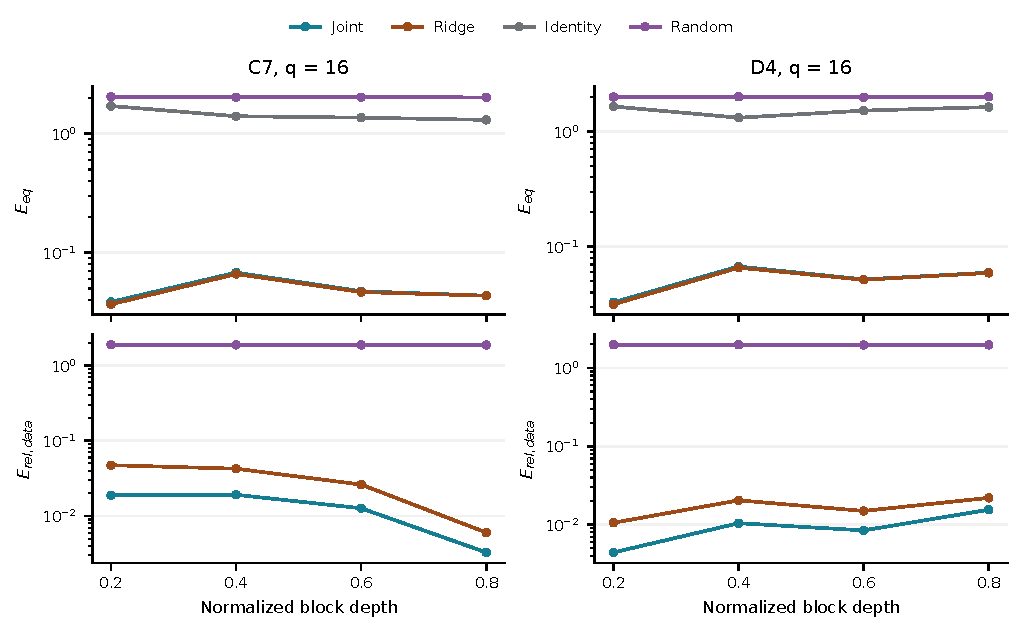
\includegraphics[width=.85\textwidth]
{figures/structural_errors.pdf}
\caption{
Historical FULL prediction and relation diagnostics
across the fixed six-model panel at $q=16$.
Identity relation scores were not evaluated and are
omitted as unavailable, rather than assigned zero.
Joint fitting changes the prediction--consistency tradeoff.
These diagnostics alone do not establish an exact action
or identify a uniquely supported state correspondence.
}
\label{fig:historical-structural}
\end{figure}

\begin{figure}[t]
\centering
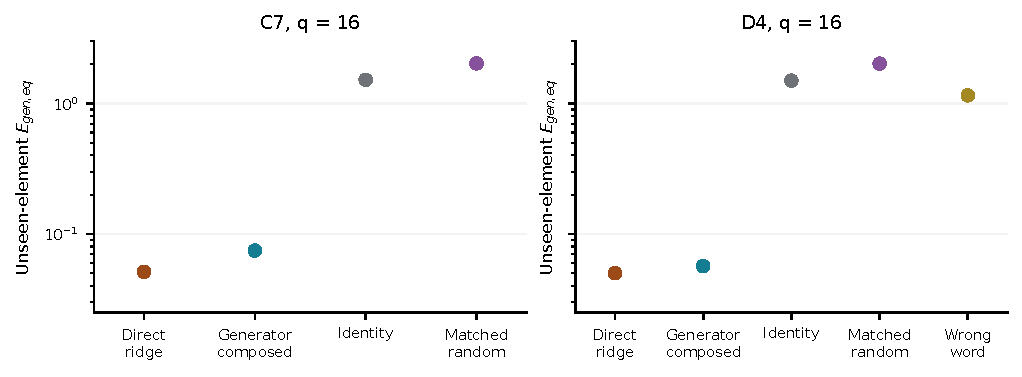
\includegraphics[width=.85\textwidth]
{figures/generator_transfer.pdf}
\caption{
AFS-A generator-composed predictions evaluated against
transformed held-out activations.
Direct element-specific Ridge receives additional
supervision.
The historical label ``Matched random'' denotes products
of randomly sampled orthogonal generator matrices using
the same evaluated words; it does not denote matching
in prediction error.
Identity, random-generator products, and the D4
length-matched wrong words address different alternatives.
}
\label{fig:historical-generator}
\end{figure}

The FULL Joint-minus-Ridge contrasts in the data-space
relation diagnostic $\Erel$ are
$-0.01699$ ($[-0.03405,-0.00318]$) for $C_7$ and
$-0.00728$ ($[-0.01248,-0.00259]$) for $D_4$.
Thus Joint has smaller mean relation defects under
this metric.
These are approximate relations evaluated on activations,
not certificates that the fitted matrices define exact
representations on the ambient coordinate space.
In AFS-A, the D4 correct-minus-wrong-word contrast in
held-out generator-composed prediction error
$E_{\mathrm{gen,eq}}$ is
$-1.097329$ ($[-1.219881,-0.953809]$).
Both words are scored against the same prescribed
held-out targets; this is a prediction contrast,
not a relation-defect contrast.

The FULL paired Joint-minus-random contrasts in $\Eeq$
are $-1.9803$ ($[-2.0041,-1.9549]$) for $C_7$ and
$-1.9449$ ($[-1.9562,-1.9325]$) for $D_4$.
The corresponding Joint-minus-identity contrasts are
$-1.3964$ ($[-1.5882,-1.1982]$) and
$-1.4771$ ($[-1.6692,-1.2628]$).
These panel averages show useful transformation prediction
relative to the untrained controls.
Joint-minus-Ridge prediction contrasts are slightly
positive:
$0.001046$ ($[0.000106,0.002285]$) for $C_7$ and
$0.000864$ ($[0.000149,0.001735]$) for $D_4$.
Joint therefore has slightly higher mean prediction error
than independent Ridge in this comparison.

The paired Joint-minus-Ridge contrasts in the data-space
homomorphism diagnostic $\Ehom$ are
$-0.000884$ ($[-0.002083,-0.000018]$) for $C_7$ and
$-0.000891$ ($[-0.001652,-0.000232]$) for $D_4$.
Together with the relation contrasts, these results
describe a tradeoff between predictive fit and the
consistency terms encouraged by Joint training.
The percentile ranges lie on one side of zero under
the recorded resampling procedure; this does not supply
calibrated population inference or resolve the
identification alternatives in \cref{sec:boundaries}.

\begin{table}[t]
\caption{
Recorded FULL consistency diagnostics at $q=16$.
Each entry pairs a data-space diagnostic with its
operator-space counterpart.
Data defects use squared discrepancies, whereas operator
defects use unsquared relative Frobenius norms.
Their normalizations and relation definitions are
specified in \cref{app:metrics}; in particular, the
$C_7$ relation aggregands differ.
The paired values are therefore not on a common
numerical scale.
Composition diagnostics require both group-element
factors to be nonidentity, but retain pairs whose
product is the identity.
}
\label{tab:full-diagnostics}
\centering
\small
\begin{tabular}{llccc}
\toprule
Group & Estimator
& $\Ehom/\Ehomop$
& $\Erel/\Erelop$
& $\Ecomp/\Ecompop$ \\
\midrule
$C_7$ & Joint
& 0.00842 / 0.05850
& 0.01348 / 0.09612
& 0.01145 / 0.07879 \\
$C_7$ & Ridge
& 0.00930 / 0.06202
& 0.03047 / 0.20903
& 0.01266 / 0.08438 \\
$C_7$ & Random
& 1.45937 / 1.03612
& 1.87118 / 1.45048
& 1.98636 / 1.41027 \\
$D_4$ & Joint
& 0.00366 / 0.10143
& 0.00971 / 0.17124
& 0.00477 / 0.13149 \\
$D_4$ & Ridge
& 0.00455 / 0.11897
& 0.01699 / 0.26283
& 0.00594 / 0.15530 \\
$D_4$ & Random
& 1.52346 / 1.08021
& 1.96710 / 1.39203
& 1.98983 / 1.41088 \\
\bottomrule
\end{tabular}
\end{table}

\begin{table*}[t]
\caption{
Historical correspondence controls and the global
additive-field reference.
AFS-B permutes group-element labels of a fixed fitted
matrix family using a restricted reference that excludes
automorphisms.
Its denominator of 120 is six models times four depths
times five splits, not 120 candidate state-action images.
The observed and reference assignments are not established
as exchangeable, so the percentile comparison is not a
calibrated semantic-null test.
AFS-C reports real-minus-scrambled test prediction error
after refitting on perturbed training pairs and evaluating
against unchanged true targets; negative values favor
the real correspondence.
Brackets are the recorded 95\% bootstrap percentile ranges.
The global additive estimator vanishes analytically
on balanced complete state orbits.
}
\label{tab:diagnostic-controls}
\centering
\small
\begin{tabular}{llp{0.49\textwidth}}
\toprule
Control & Group/metric & Recorded summary \\
\midrule
AFS-B & $C_7$, data homomorphism
& 120/120 below reference 2.5th percentile \\
AFS-B & $C_7$, operator homomorphism
& 120/120 below reference 2.5th percentile \\
AFS-B & $D_4$, data homomorphism
& 120/120 below reference 2.5th percentile \\
AFS-B & $D_4$, operator homomorphism
& 120/120 below reference 2.5th percentile \\
AFS-C & $C_7$, state relabel
& $-0.577\;[-0.664,\,-0.488]$ \\
AFS-C & $C_7$, target scramble
& $-0.596\;[-0.686,\,-0.506]$ \\
AFS-C & $D_4$, state relabel
& $-0.765\;[-0.861,\,-0.662]$ \\
AFS-C & $D_4$, target scramble
& $-0.729\;[-0.824,\,-0.627]$ \\
\midrule
Global additive & Balanced complete orbit
& $\widehat v_g=0$ by permutation cancellation \\
\bottomrule
\end{tabular}
\end{table*}

AFS-B preserves the fitted matrix family while changing
which algebraic element each matrix represents.
It does not enumerate coherent state-action images or
compare their spectral budgets, as the Study~2
registration analysis does.
AFS-C instead changes the training correspondence while
retaining the activation multiset, refits Ridge, and
scores it against the true held-out targets.
In both groups and both AFS-C scramble variants,
the recorded mean test prediction and data-relation
defects increase.
The latter are consistency diagnostics on held-out
activations, not additional measurements of semantic-target
prediction accuracy.

In AFS-C, prediction error and operator norms are not
matched across conditions.
Moreover, the $C_7$ power-consistency and $D_4$ $srs$
terms normalize by condition-specific fitted outputs.
Their deterioration therefore does not isolate an
algebraic effect beyond the change in predictive fit.
Neither AFS-B nor AFS-C shows that a coherently registered
alternative action with comparable learnability
would fail.


\subsection{Rank-matched lexical comparison}

AFS-D compares lexical embeddings with internal
representations using independent Ridge.
Both locations retain training projected rank $q=6$
for $C_7$ and $q=3$ for $D_4$.
This two-model comparison is separate from the FULL
analysis at $q=16$.
The audited input spectra and recorded PCA procedure
support the training-rank match; the historical projected
arrays are unavailable for direct remeasurement
(\cref{app:dimension-rank-audit}).

\begin{table*}[t]
\caption{
Rank-matched lexical and internal comparison using
independent Ridge.
The generator-composed endpoint $E_{\mathrm{gen,eq}}$
uses the five elements excluded from generator fitting.
Both locations use $q=6$ for $C_7$ and $q=3$ for $D_4$;
these are not FULL $q=16$ estimates.
Internal means average four fixed depths.
Repeated embedding observations reuse the same lexical
state vectors.
Equal retained rank does not imply equal retention
of total variance or state-dependent information.
}
\label{tab:lexical-control}
\centering
\small
\begin{tabular}{lllrrr}
\toprule
Group & Model & Location
& $\Eeq$ & $E_{\mathrm{gen,eq}}$ & $\Erel$ \\
\midrule
$C_7$ & Llama 1B & Embedding
& $3.64\!\times\!10^{-6}$
& $5.87\!\times\!10^{-5}$
& $6.37\!\times\!10^{-5}$ \\
$C_7$ & Llama 1B & Internal mean
& 0.132327 & 0.198978 & 0.092076 \\
$C_7$ & Qwen 1.5B & Embedding
& $2.48\!\times\!10^{-6}$
& $4.25\!\times\!10^{-5}$
& $4.72\!\times\!10^{-5}$ \\
$C_7$ & Qwen 1.5B & Internal mean
& 0.171656 & 0.315743 & 0.187296 \\
\midrule
$D_4$ & Llama 1B & Embedding
& $4.97\!\times\!10^{-7}$
& $2.97\!\times\!10^{-6}$
& $3.95\!\times\!10^{-6}$ \\
$D_4$ & Llama 1B & Internal mean
& 0.096634 & 0.133246 & 0.051652 \\
$D_4$ & Qwen 1.5B & Embedding
& $3.02\!\times\!10^{-7}$
& $1.80\!\times\!10^{-6}$
& $2.39\!\times\!10^{-6}$ \\
$D_4$ & Qwen 1.5B & Internal mean
& 0.055191 & 0.059383 & 0.027160 \\
\bottomrule
\end{tabular}
\end{table*}

\begin{figure}[t]
\centering
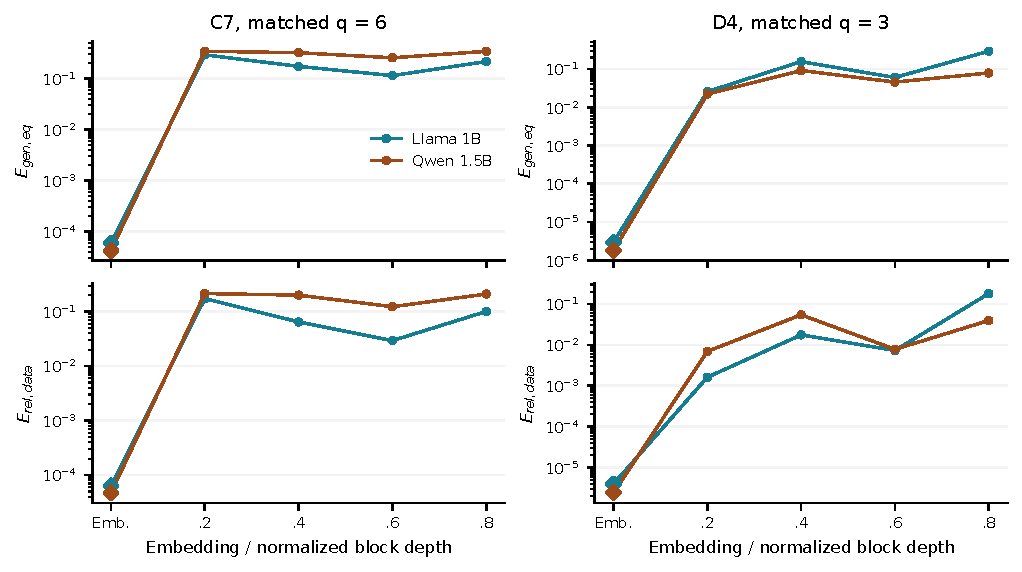
\includegraphics[width=.76\textwidth]
{figures/lexical_internal.pdf}
\caption{
AFS-D lexical and internal errors at matched training
projected rank: $q=6$ for $C_7$ and $q=3$ for $D_4$.
The upper row shows generator-composed prediction error
$E_{\mathrm{gen,eq}}$ on the five excluded elements;
the lower row shows $\Erel$.
The logarithmic axes display descriptive mean errors.
The comparison concerns two models and is separate
from FULL at $q=16$.
Lexical near-exactness is compatible with finite-state
realizability and does not establish a uniquely
supported semantic correspondence.
}
\label{fig:lexical}
\end{figure}

Across the two models and two groups, the
internal-minus-embedding contrasts are positive for
prediction and data-relation error.
Internal representations therefore do not improve these
errors over lexical embeddings under this recorded
rank-matched protocol.
More broadly, all 150 archived metric/depth-summary
intervals have positive lower endpoints.
These comprise 120 depth-specific intervals and
30 intervals for depth-averaged summaries:
two models, six $C_7$ metrics or nine $D_4$ metrics,
and four depths plus their average.
They include metrics not displayed in
\cref{tab:lexical-control}.
They are related summaries of reused observations,
not 150 independent experiments or tests
(\cref{app:inference}).

This comparison does not show that the lexical vectors
encode the uniquely correct semantic action.
For affinely independent lexical state vectors,
retaining the full $(n-1)$-dimensional centered span
permits every state permutation to be realized by a
linear map on that span.
Nor do the observed error differences establish that
internal representations contain less state information.
The result depends on the retained coordinates,
fitting procedure, and evaluation loss.
It does not extend automatically to other models,
dimensions, readout positions, or context constructions.


\subsection{Global additive-field results}

The global additive-field comparator assigns one
source-independent displacement to each group element.
Its recorded direct prediction error is $1.487859$,
compared with $0.050149$ for Ridge and $0.051104$
for Joint.
The additive-minus-Ridge contrast is
$1.437710$ ($[1.400230,1.475673]$), and the
additive-minus-Joint contrast is
$1.436755$ ($[1.399237,1.474462]$).

For these direct-error summaries, the analysis averages
the evaluated actions within each domain and condition,
gives equal weight to model--depth conditions and
domains within each split, and then averages the
five split summaries.
The Ridge and Joint point estimates coincide with
the equal-domain averages of the primary FULL means.
The additive point estimate coincides with the
corresponding identity baseline.
The uncertainty calculations differ:
the additive-field analysis resamples five paired
split-level contrasts, whereas FULL uses the
hierarchy in \cref{app:inference}.

The repeated-composition comparisons use the Ridge
and Joint matrices from FULL, where all elements
were fitted.
They are not additional AFS-A generator-only results.
For $C_7$ powers $r^k$, $k=2,\ldots,6$, the mean
errors are $1.519200$, $0.074443$, and $0.070297$
for additive, Ridge, and Joint, respectively.
For the combined D4 application sequences
$r\to s$, $s\to r$, and $s\to r\to s$,
the corresponding errors are
$1.266128$, $0.049265$, and $0.047450$.
The arrows here specify the order in which the
updates are applied.

The global displacement estimator vanishes for every
group element because the training set contains
complete, balanced state orbits.
For each template, a permutation preserves the sum
of the state vectors, so
\[
 \sum_{i\in S}
 \bigl(h_{g(i),t}-h_{i,t}\bigr)=0.
\]
Averaging these differences over states and templates
therefore gives $\widehat v_g=0$.
The fitted global additive predictor consequently
reduces to identity, and repeated updates remain
identity.
Its failure already occurs for the cyclic task.
The D4 result therefore does not isolate an effect
of noncommutativity, although the commutativity
of translations is an additional limitation of
this edit class.
The result does not rule out source-conditioned
or other additive predictors.

The D4 order-separation diagnostic compares the
outputs of the two application sequences
$r\to s$ and $s\to r$ using
\[
 s(a,b)=
 \frac{\|a-b\|_2^2}
 {\tfrac12\bigl(\|a\|_2^2+\|b\|_2^2\bigr)+10^{-12}}.
\]
Each method uses its own two output vectors in
both the numerator and denominator.
The recorded mean separation is $2.2133$ for the
actual contextual targets, $2.2789$ for Ridge
predictions, and $2.2526$ for Joint predictions.
The additive separation is zero by construction.
These are descriptive separation scores under a
symmetric energy normalization.
They are neither the row-target-normalized loss
$D$ nor prediction accuracies, and they are not
independent confirmatory tests.


\subsection{Behavioral patching}
\label{app:behavior}

The evaluation prompt appends
`` Report the transformed state:''
to a held-out structural prompt.
The source state remains visible.
The particular transformation is supplied through
the selected activation intervention, rather than
through an explicit textual instruction naming $g$.
This setup tests the downstream effects of an
externally chosen edit; it does not establish
which transformation the unpatched model would
compute on its own.

The learned edits use the FULL Joint matrices,
trained with supervision for all group elements.
Let $M_w$ denote the matrix applied in an intervention,
which may be a directly fitted matrix or a product
specified by a word $w$.
This distinction matters when a composed word,
a direct reference, and a wrong-word control
are compared.
Let $\bar h$ be the mean hidden vector over the
selected state span in the evaluation prompt,
let $U_{\mathrm{PCA}}$ be the structural training-only
PCA basis, and define
\[
 z=(\bar h-\hat\mu)U_{\mathrm{PCA}}.
\]
The replacement vector is
\[
 h'
 =
 \bar h-zU_{\mathrm{PCA}}^\top
 +(zM_w)U_{\mathrm{PCA}}^\top.
\]
The forward hook writes this vector to every token
position overlapping the state string at the selected
transformer block output, then recomputes the
remaining network.

The historical control called ``Identity'' uses the
original unpatched output.
It is not an identity-matrix patch.
If the state span contains multiple tokens with
vectors $h_j$, the intervention satisfies
\[
 h'-h_j
 =
 (zM_w-z)U_{\mathrm{PCA}}^\top
 - (h_j-\bar h).
\]
Thus only the change to the span mean is restricted
to the retained PCA subspace.
Writing the same vector to all selected positions
also removes token-specific deviations from the mean,
which need not lie in that subspace.
Even setting $M_w=I$ need not reproduce the
unpatched computation.
The historical experiment contains no matched
zero-delta or token-deviation-preserving sham.
The one-token continuation counts reported below
do not establish that the input state spans
contain one token.

The source-conditioned additive comparator is fitted
on structural training prompts in the original
hidden dimension:
\[
 v_{g,i}
 =
 \frac{1}{|\mathcal T_{\mathrm{train}}|}
 \sum_{t\in\mathcal T_{\mathrm{train}}}
 \bigl(h_{g(i),t}-h_{i,t}\bigr),
 \qquad
 h'=\bar h+v_{g,i}.
\]
It uses the known source-state identity and one
displacement per group-element/source-state pair.
It therefore has different information and
parameterization from a source-shared linear map.
The two edit classes are not generally nested:
the additive displacement is conditioned on the
state label, whereas a shared linear map can
respond to contextual variation in its input.
The additive displacement acts in the original
hidden space, while the learned matrix changes
the PCA component of the span mean.
This comparison avoids global orbit-averaging
cancellation, but it is not a parameter-,
information-, or edit-subspace-matched test of
steering optimality.

In the recorded D4 relation rows, the additive
comparator is indexed by the requested target element.
The true word, its direct reference, and the wrong
word therefore receive the same endpoint-conditioned
displacement.
Their equality for this comparator follows from
the construction and does not test additive
composition order.

The target-token score uses the first token of the
context-sensitive continuation `` \{target state\}''.
Target-logit and target-probability changes subtract
the corresponding values from the unpatched prompt.
The margin is the target first-token logit minus
the original-state first-token logit.
Top-1 success requires the vocabulary argmax to
equal the target token.
The implementation records full target-sequence
log probability only for one-token continuations
and omits that metric for multi-token continuations.
All archived evaluated continuations contain one
token.
These top-1 results therefore concern the scored
continuation token, not general multi-token
answer accuracy.

\begin{table*}[t]
\caption{
Behavioral contrasts from externally applied FULL
Joint edits.
The first four rows summarize transformation
interventions: $r^1,\ldots,r^6$ for $C_7$ and
$r,s,r^2,r^3$ for $D_4$.
Cycle and relation diagnostics are evaluated separately.
``Unpatched'' is the baseline called ``Identity''
in the historical outputs.
Additive denotes the training-only source- and
transformation-conditioned comparator, not the
global additive field.
Positive logit or top-1 differences favor the
learned edit; pp denotes percentage points.
Brackets give the recorded 95\% bootstrap percentile
ranges, interpreted as fixed-panel resampling
sensitivity (\cref{app:inference}).
}
\label{tab:causal-main}
\centering
\small
\begin{tabular}{llll}
\toprule
Group & Metric
& \shortstack{Learned minus\\unpatched}
& \shortstack{Learned minus\\additive} \\
\midrule
$C_7$ & Target logit
& $1.129\;[0.791,\,1.400]$
& $-0.105\;[-0.227,\,-0.014]$ \\
$C_7$ & Top-1 (pp)
& $1.743\;[-0.215,\,3.945]$
& $-0.261\;[-1.065,\,0.056]$ \\
$D_4$ & Target logit
& $2.406\;[1.932,\,2.833]$
& $-0.007\;[-0.030,\,0.012]$ \\
$D_4$ & Top-1 (pp)
& $9.019\;[3.186,\,15.339]$
& $-0.043\;[-0.503,\,0.434]$ \\
\midrule
\multicolumn{4}{l}{
$D_4$ correct-minus-wrong final-logit distance:
$-0.0422\;[-0.0543,\,-0.0298]$.
} \\
\bottomrule
\end{tabular}
\end{table*}

\begin{figure}[t]
\centering
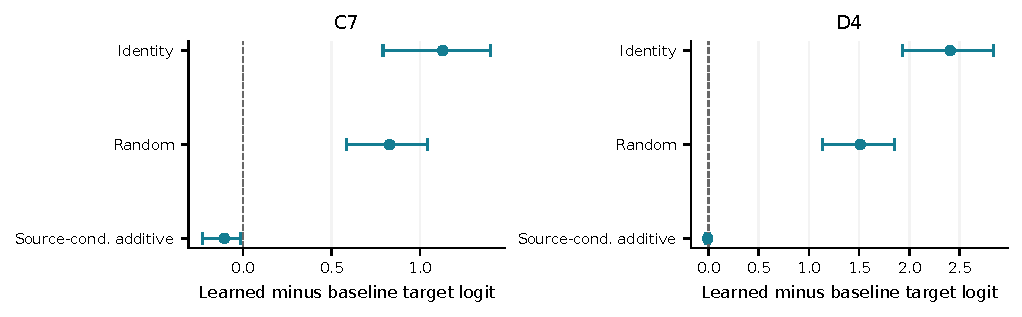
\includegraphics[width=.76\textwidth]
{figures/causal_additive.pdf}
\caption{
Learned-minus-control target-logit contrasts for
transformation interventions.
The historical figure label ``Identity'' denotes
the unpatched baseline.
The other controls use random-generator products
and source-conditioned additive edits.
Negative differences favor the named control
for this outcome.
Bars retain the recorded 95\% bootstrap percentile
ranges.
These downstream effects do not demonstrate
causal necessity of the learned matrix family.
}
\label{fig:causal}
\end{figure}

For $C_7$, powers $r^1,\ldots,r^6$ are transformation
interventions, while $r^7$ is a separate cycle
diagnostic.
For $D_4$, transformation interventions use
$r,s,r^2,r^3$.
The identity-recovery words are $r^4$ and $s^2$,
and the relation diagnostic compares the word
$srs$ with a direct $r^{-1}$ intervention.
The length-matched wrong word is $rsr$.
Although $srs$ and $rsr$ represent different group
elements, they have the same target on two of the
four corners; the wrong-word control does not
change the target for every source state
(\cref{app:faithful-not-free}).

For final next-token logit vectors $L$, the
relation distance is
\[
 d(w,r^{-1})
 =
 \frac{\|L^{(w)}-L^{(r^{-1})}\|_2}
 {\max\bigl(\|L^{(r^{-1})}\|_2,\epsilon\bigr)},
\]
where $\epsilon$ is float64 machine epsilon in
the recorded implementation.
The correct-minus-wrong distance contrast is
$-0.04220$ ($[-0.05426,-0.02981]$).
Both words are compared with the same direct
learned reference.
This is an order-sensitive downstream consistency
diagnostic, not a comparison with a uniquely
identified causal mechanism.

For $C_7$ transformation interventions, the
learned-minus-unpatched target-logit contrast is
$1.129$ ($[0.791,1.400]$), and the
learned-minus-random contrast is
$0.828$ ($[0.585,1.041]$).
The C7 top-1 contrast against the unpatched
baseline has a percentile range spanning zero.
The corresponding D4 top-1 contrast is
$9.019$ percentage points ($[3.186,15.339]$).
The learned-minus-additive target-logit range
lies below zero for $C_7$ and spans zero for
$D_4$.
These observations do not establish a uniform
advantage of the learned edits over the
source-conditioned additive comparator.
A range spanning zero also does not establish
equivalence.

The results show that these interventions can
affect the scored outputs, while leaving substantial
ambiguity about native computation.
The distinction between an editable representation
and the mechanism used by the unpatched model
also matters when interpreting calendar and
group-operation interventions
\citep{engels2025notall,wu2025unified,feucht2026arithmetic}.
Here the transformation is externally selected,
and the intervention and comparator differences
prevent a claim of causal necessity for the
fitted operator family.

\FloatBarrier


\subsection{Cross-model compatibility}

The analysis uses nine fixed model pairs:
all three within-Llama pairs, all three within-Qwen
pairs, and the three size-matched cross-family
pairs, 1B/1.5B, 3B/3B, and 8B/7B.
The operator families are the FULL Joint fits.
For two systems $R_A,R_B$, a row-coordinate
map $T$ is assessed through
\[
 R_A(g)T \approx T R_B(g).
\]
The implementation writes $T=P^\top$ and stacks
the residuals
\[
 P R_A(g)^\top-R_B(g)^\top P.
\]
The smallest right singular vector minimizes
their summed squared Frobenius norm subject to
$\|P\|_F=1$.
This optimization permits singular or low-rank
maps; it does not require an invertible
change of coordinates.

Evaluation reports the normalized score
\[
 \frac{
 \mathbb E_g
 \|P R_A(g)^\top-R_B(g)^\top P\|_F^2
 }{
 \mathbb E_g\|R_B(g)^\top P\|_F^2+10^{-12}
 }.
\]
The singular-vector solution minimizes the
unnormalized numerator, not this ratio.
A small score can therefore indicate compatibility
on a low-rank common subspace without establishing
equivalence of the full representations.

The comparators are an orthogonal Procrustes map,
random orthogonal maps, and shuffled group labels.
Procrustes is fitted to registered test-template
activation pairs after centering their retained
16-dimensional PCA coordinates.
It optimizes activation reconstruction.
The intertwiner instead fits the operators using
the same group elements on which its residual
is reported.
The comparison is therefore descriptive and
uses two fitting criteria on different objects;
it is not predictive transport to unseen paired
activations or held-out elements.
The shuffled-label control retains the map fitted
under the true labels rather than refitting it
after shuffling.
It tests the sensitivity of that map to the
assignment of group labels, not the best achievable
fit under each alternative assignment.
Some shuffled-label comparisons can also be
near-degenerate.

The fitted-minus-Procrustes normalized residual
differences range approximately from $-0.168$
to $-0.065$ across the four domain-by-pair-type
strata: $C_7$ or $D_4$, each with within-family
or cross-family pairs.
All four recorded percentile ranges lie below
zero.
These are stratum-level contrasts, not a claim
that every model--depth--split observation favors
the fitted map.
They show that the fitted commutation maps have
lower mean reported residuals than the selected
geometry alignments in these comparisons.
They do not establish invertible cross-model
representation equivalence.

Linear CKA is computed on the full hidden readouts
before PCA, whereas the commutation score uses
the fitted 16-dimensional operator systems.
The recorded Spearman association between CKA
and negative fitted commutation error is
$-0.014$, with percentile range
$[-0.300,0.287]$.
The pooled calculation contains 360 observations:
nine model pairs, two domains, four depths,
and five splits.
These are not 360 independent samples.
The 5,000 bootstrap draws resample model pair,
then depth, then split, keeping the two domains
together within each terminal block.
The range describes sensitivity under that
historical procedure and does not establish
statistical independence of geometry and
operator compatibility.

Unlike implementation-family comparisons based
on causal abstractions and Congruity
\citep{sun2026tracking}, this analysis neither
samples behavior-preserving implementations nor
estimates an abstraction-dependent distance
between them.
Its scope is compatibility of the fitted
operator systems under the stated map classes
and evaluation criteria.


\subsection{Completed controls and remaining identification scope}

Study~2 provides state-centroid, residual, and
input-only field comparisons under its own
sampling and normalization contract.
Completed extensions include compact nonlinear
predictors fitted on the full training data,
coherent alternative registrations, direct
context-difference fitting, and peer-method
adaptations (\cref{app:reproduction}).
These results add evidence under their respective
protocols.
They do not remove information, fitting, or
intervention mismatches in the historical
Study~1 comparisons.

The new-context study evaluates transport to
64 assistant-authored paired families per domain
while retaining the previously seen state
vocabulary (\cref{sec:new-context}).
The original and new comparisons differ in
wording, validation-based regularization selection,
and, for $D_4$, action weighting.
Their contrast therefore does not isolate a
causal effect of new wording.
The new bank extends the evaluated context
construction, but it does not establish
cross-vocabulary generalization or transport
to independently sampled human-authored prose.
The fitting and paired-family resampling
procedures are given in
\cref{app:pending-protocols}.

The within-template centering diagnostic adds a
separate qualification to registration preference
(\cref{app:template-centering-sensitivity}).
Using the saved 16-dimensional Study~2 coordinates,
the prescribed weekday image is uniquely leading
by spectral budget in 7/24 original conditions,
15/24 after centering with the original whitening,
and 18/24 after centering and rewhitening.
The corresponding corner counts are 16/24,
0/24, and 0/24
(\cref{tab:template-centering-main}).
For corners, the loss of the original lead
therefore occurs even when the original
whitening metric is retained.

These are rankings by $s_{16}=C_{16}/16$,
not rankings of the unknown exact-action risks
$L^\star$.
Under fixed whitening, removing the state-invariant
component preserves the nontrivial spectral blocks
but changes their competition for the dimension
budget.
Rewhitening additionally changes the metric.
The fixed-whitening centered score is not
substituted into the unit-second-moment risk
bounds.
The ranking changes neither establish that
exact actions cease to exist nor measure
state variation outside the retained PCA space.
They show that the observed registration
preference depends on the state-invariant
component and the metric used to evaluate
the retained representations.

The remaining identification gaps should be
distinguished from the finite-bank results
already established.
Interpreting the historical fitted consistency
diagnostics as additional evidence of semantic
specificity would require controls matched
more closely in direct prediction error and
operator norms.
This limitation does not invalidate the
same-bank bounds on the cost of exact-action
constraints.
Cross-vocabulary generalization requires new
lexical realizations, while broader context
generalization requires additional independently
constructed language settings.
Native causal use requires counterfactual
evidence in a task the unpatched model performs
competently.
Native confirmation remains blocked despite
the completed secondary peer-method adaptations.
It is not inferred from the present activation
edits.

Future method selection using the already
inspected holdout would be exploratory and
would require fresh evaluation before a
confirmatory interpretation.
A wrong-group comparator must also admit the
claimed action on the state set.
For example, no permutation of four states
has order eight, so $C_8$ cannot act faithfully
on the four corners.
Nonfaithful actions through smaller quotients
remain possible and are not excluded by the
exact-action class.
An impossible faithful comparator is not an
error-matched semantic alternative.

\section{Study 2: Coordinate Banks and Original Characterization}
\label{app:characterization}

This appendix retains the original coordinate characterization,
which was specified after the excluded development comparisons.
It contains 72 model--readout--domain cells:
six models, four readouts, and three domains.
The 120 evaluation records comprise one C7 stratum, one D4
stratum, and three S3 strata in each of the 24 model/readout
conditions; they are not 120 independent random partitions.
The input-only field comparisons cover the 48 C7/D4 cells.
The results are descriptive aggregates of inspected outputs.
Original source flags and failed decisions remain in the archive,
and these outputs cannot serve as untouched data for later
method selection.
The later compact, transport, and spectral analyses retain
their separate evaluation contracts.

\paragraph{Data and information conditions.}
All six pinned base models use four readouts and training-only
$q=16$ PCA coordinates.
Model extraction uses BF16 and coordinate analysis uses float64.
The original execution added 41,728 extracted rows per model:
896 C7, 512 D4, and 40,320 S3 rows, including separately charged
support.
These are newly extracted rows in that execution, not the size
of the complete merged training, validation, and test banks.
For C7/D4, training and validation reuse the construction
caches, while the added rows form 64 test families with two
variants and complete state sets.
This original test construction is distinct from the later
64-family authored bank in \cref{sec:new-context}.

The S3 task permutes the assignments of three entities to
three roles, giving six abstract assignment states.
Its new-context, new-entity, and jointly new strata contain
$64\times24$, $48\times16$, and $64\times16$ family/entity
combinations, respectively.
Each combination has two variants and six states.
The resulting row counts are 18,432, 9,216, and 12,288;
384 additional support rows complete the total of 40,320.
The C7/D4 readout averages the state-token span.
S3 instead uses the final-token representation after the
complete role-assignment prompt.
New S3 entities therefore test transfer to held-out names
and triples while retaining the six abstract assignment states.
The C7/D4 state vocabulary is already seen in construction.
Holding out composite actions does not hold out those state
identities or create independently authored grammar roots.

Coordinate fields receive source coordinates and a requested
action, with supervised source--target training pairs.
The decoded-centroid benchmark additionally receives training
state labels and the exact action table, but decodes the
source state at evaluation.
The prediction contrasts in
\cref{tab:characterization-intervals} instead use
validation-selected oracle-source category/retention controls,
with an input-metadata potential also available for S3.
These are distinct information conditions.

\paragraph{Losses, fitting, and aggregation.}
The characterization normalizes squared errors by training-only
energy scales.
The Study~1 loss $D$ in \cref{eq:D} instead normalizes each row
by its target energy, so values across these studies are not
interchangeable.
Writing $\bar z_{\rm tr}$ for the training coordinate mean,
define
\[
 E_z=\mathbb E_{\rm tr}\|z-\bar z_{\rm tr}\|_2^2.
\]
For the two paraphrases of a family, ordered by their
registered identifiers, set
\[
 u_i=z_{p_0,i}-z_{p_1,i},
 \qquad E_u=\mathbb E_{\rm tr}\|u_i\|_2^2,
\]
without recentering the differences.
Coordinate prediction uses
$\|\widehat z_g-z_{g(i)}\|_2^2/E_z$.
The context endpoint fits a separate family of linear maps
$Q_g$ directly to training difference pairs $(u_i,u_{g(i)})$.
Its row-level contrast is
\[
 \Delta_{\rm ctx}(i,g)
 =
 \frac{\|\alpha u_i-u_{g(i)}\|_2^2
       -\|u_iQ_g-u_{g(i)}\|_2^2}{E_u},
\]
where the scalar-retention coefficient $\alpha$ is selected
separately on validation data.
Positive values favor the difference-fitted map.
The coordinate and difference fits each select one ridge
coefficient shared across actions within their condition.
Thus the original context contrast is difference fitting
versus scalar retention, not the later comparison of
difference fitting with coordinate fitting.

For prediction and context endpoints, validation and evaluation
retain changed-state pairs, $g(i)\ne i$.
All-element fitting uses all training pairs, including
identity and fixed-point pairs.
Generator-only fitting and selection use only the primitives.
The separate cycle and relation diagnostics have their own
complete-state evaluation rules.
Study~1's nonidentity-action prediction average retains D4
fixed-point pairs; the primary endpoints here exclude them.

Validation selection first averages changed-state errors
within each action and then gives actions equal weight.
The original reported prediction and context summaries
instead pool changed-state pairs within each family/entity
unit.
D4 actions move different numbers of corners, so these two
weightings need not agree.
The later compact endpoint uses equal-action evaluation
(\cref{app:aggregation-contract}).
Neither endpoint is the complete-bank, full-group,
second-moment-whitened class risk of
\cref{eq:class-loss-main}.

For resampling, the 24 fixed model/readout conditions are
first averaged within each family/entity unit.
The grids are $64\times1$ for C7/D4,
$64\times16$ for jointly new S3 contexts/entities,
$64\times24$ for new S3 contexts, and
$48\times16$ for new S3 entities.
The C7/D4 single column is a placeholder for family-only
resampling.
S3 independently resamples the family and entity indices.
The 10,000 percentile draws use seed 314159 and keep fitted
predictors and selected parameters fixed.
They do not repeat fitting or selection, sample a population
of models, or supply calibrated superiority, equivalence,
or multiplicity-controlled decisions.
\begin{table}[htbp]
\caption{Original characterization contrasts on the grammar-derived held-out banks, with recorded 95\% percentile sensitivity intervals (10,000 draws, seed 314159). Prediction compares validation-selected oracle-source category/retention controls, additionally including the S3 input-metadata potential, with coordinate Ridge. Context compares scalar retention with maps fitted directly to training paraphrase differences. Each contrast is baseline minus fitted-map loss, so positive values favor the fitted map. The endpoints use different training-energy denominators and pool changed-state pairs. Fitted models and selections remain fixed during family or crossed family/entity resampling. These banks and comparators differ from the later authored-context study.}
\label{tab:characterization-intervals}\centering\small
\begin{tabular}{llrrr}\toprule
Domain / split & Endpoint & Baseline minus linear & Lower & Upper \\
\midrule
$C_7$, new context & prediction & -0.002887 & -0.003290 & -0.002495 \\
$C_7$, new context & context & 0.011485 & 0.009997 & 0.013087 \\
$D_4$, new context & prediction & 0.019612 & 0.014730 & 0.025945 \\
$D_4$, new context & context & 0.060918 & 0.049883 & 0.072920 \\
$S_3$, context & prediction & -0.000487 & -0.000791 & -0.000249 \\
$S_3$, context & context & 0.000177 & 0.000010 & 0.000348 \\
$S_3$, entity & prediction & 0.000673 & 0.000443 & 0.000927 \\
$S_3$, entity & context & 0.000739 & 0.000542 & 0.000978 \\
$S_3$, joint & prediction & 0.000460 & 0.000262 & 0.000673 \\
$S_3$, joint & context & 0.000154 & -0.000017 & 0.000338 \\
\bottomrule\end{tabular}
\end{table}


\paragraph{Prediction and compact category controls.}
All-element direct Ridge and full-support kernel means are
$0.014900/0.004626$ for C7 and $0.041349/0.020916$ for D4.
Let $\mu_i$ be the training centroid for state $i$, and define
the nearest-centroid decoder and displacement predictor by
\[
 \widehat i(z)=\arg\min_{i\in S}\|z-\mu_i\|_2,
 \qquad
 \widehat z_g
 =z+\mu_{g(\widehat i(z))}-\mu_{\widehat i(z)}.
\]
Source decoding is perfect on the observed validation and
test input coordinates in all 48 C7/D4 field conditions.
The C7 mean error is $0.012013$, below Ridge's mean but
lower in only 9/24 conditions.
The D4 mean is $0.062349$, above Ridge's mean and lower
in only 2/24 conditions.
These original pooled endpoints differ from the later
compact comparison, including its D4 centroid/Ridge means
$0.063821/0.041919$ (\cref{app:aggregation-contract}).

The centroids store 112 and 64 floating-point coordinates
for C7 and D4, respectively, in addition to the integer
action table and decoding procedure.
This is a compact predictive control with explicit
construction labels, unlike fields that receive paired
targets but no explicit state labels.
Its accuracy does not establish native centroid decoding.
Applying a known composite label after one decode is also
different from repeatedly applying primitives and decoding
each intermediate output.
Perfect decoding of observed inputs does not certify that
repeated procedure.

\begin{figure}[t]
\centering
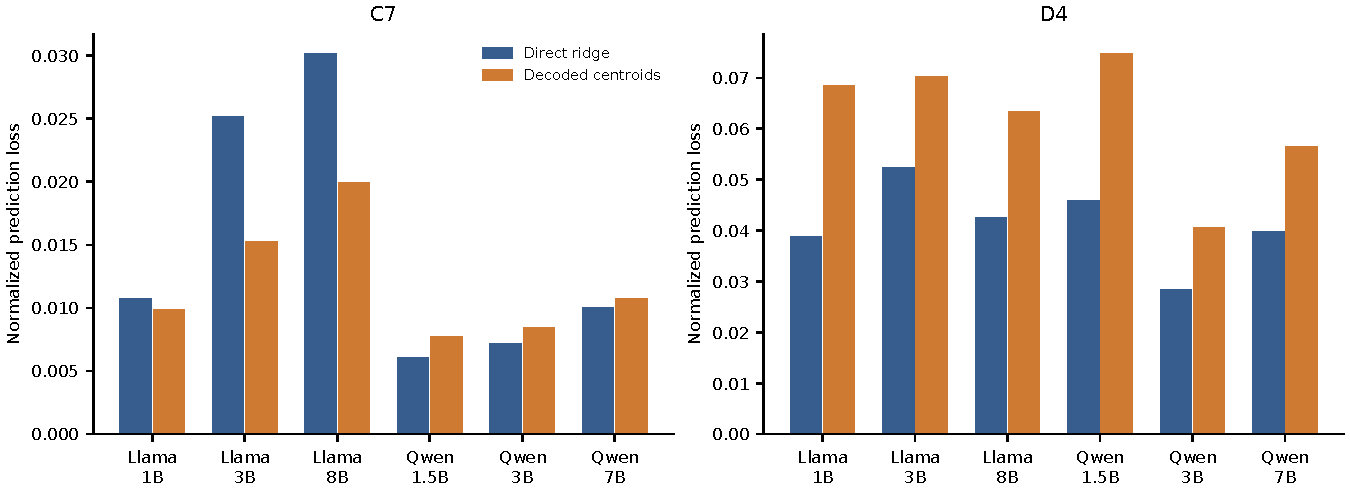
\includegraphics[width=.95\textwidth]
{figures/characterization_baselines.pdf}
\caption{
Original characterization prediction losses, pooling
changed-state pairs and averaging four fixed readouts
within each model.
C7 model means favor decoded centroids in the three
Llama models and Ridge in the three Qwen models;
D4 model means favor Ridge in all six.
These model means do not replace the condition-level
win counts and are not independent model-population draws.
The centroid predictor receives training labels and
the exact action table.
This is the original endpoint, not the later compact
comparison's equal-action aggregate.
}
\label{fig:characterization-baselines}
\end{figure}

\paragraph{Predictive accuracy and retained storage.}
The input-only field predicts a displacement by a normalized
Gaussian-weighted average of paired training displacements,
then adds it to the source coordinate.
Full support means retaining all training source points;
it does not mean using the full hidden dimension.
Primitive-only full fields store 21,504 versus 256 scalar
entries for C7 and 18,432 versus 512 for D4, relative to
the corresponding linear generator maps: factors of 84
and 36.
The small prescribed support budgets store 256 versus 256
for C7 and 480 versus 512 for D4.
The latter is near-budget rather than exactly matched.

On the original excluded-element prediction endpoint,
Ridge, full-support fields, and near-budget fields have
means $0.023176$, $0.004966$, and $0.700957$ for C7,
and $0.049005$, $0.023901$, and $0.212332$ for D4.
The lower full-support field errors therefore do not
establish an advantage at the small storage budgets.
Farthest-first support selection inspects all construction
source coordinates but retains only $K$ source points
and their paired displacements.
Linear regression instead compresses all construction
target pairs into its coefficients.
The original comparison did not train a compressed
nonlinear estimator on all target pairs.
The RFF/Nystr\"om extension in \cref{app:reproduction}
provides that separate comparison, with its own fitting,
identity handling, and aggregation.

All 48 full primitive fields select the smallest frozen
bandwidth multiplier, $0.125$; some reduced-support fits
select $0.25$.
These multipliers scale a training-source distance statistic,
rather than specify an absolute bandwidth.
Selection at the grid boundary limits what can be inferred
about the preferred scale.
A broader grid would require development-based specification,
not retrospective tuning on these test outcomes.

All-element Ridge stores a fitted identity-element matrix:
the recorded counts are 1792/2048 for C7/D4, or
1536/1792 when the identity is handled deterministically.
The $K=14$ fields store 1792/2016 entries, or 1568/1792
after removing zero identity-displacement arrays.
The pruned C7 field therefore retains 1,568 entries versus
1,536 for Ridge, about 2.1\% more.
The common PCA center and basis cost $d(q+1)$ float64
entries in this export.
Model weights, training memory, action tables, centroids,
biases, normalization, temporary arrays, and actual
precision must be accounted for where applicable.
Incremental stored-entry counts are neither total RAM
nor measures of statistical capacity.

\paragraph{S3 and context limitations.}
On the jointly new S3 context/entity stratum, identity
prediction loss is $0.018939$, compared with $0.018642$
for independent Ridge.
Here jointly new describes the evaluation stratum,
not the Joint estimator.
A small absolute loss alone is therefore weak evidence
of action recovery.
The corresponding context-contrast interval spans zero,
and the other S3 contrasts are small relative to the
original $0.01$ practical margin.
Neither observation establishes equivalence.
Support displacement gives prediction losses of
$0.015282$ on the joint stratum and $0.017580$ on new
entities, using four additional contexts per held-out
entity triple and assignment state.
These support observations are separately charged and
excluded from primary PCA and operator fitting;
the comparison is not zero-shot operator superiority.

The potential control is selected in the same 10/24
model/readout conditions across the three S3 strata,
yielding 30 stratum-specific records rather than
30 independent partitions.
Its neural optimization has not been independently
replayed.
The analytic difference fit is a separate estimator.
The original characterization adds no S3 coordinate-kernel,
native-intervention, or cross-model comparison.
Later context predictors and secondary extensions are
identified separately in \cref{app:reproduction}.

\paragraph{Relation to the later spectral diagnostics.}
The original predictive results above use their
training-derived coordinates and energy normalizations.
The spectral analysis instead characterizes complete
evaluated banks under its declared metric.
Within-template centering in
\cref{app:template-centering-sensitivity} operates only
in the saved 16-dimensional C7/D4 spaces and does not
recompute all predictors reported here.
The fixed-whitening treatment reports $C_{16}/16$
budgets and registration ranks; rewhitening additionally
changes the metric.
Neither procedure measures state-dependent variation
discarded outside the retained space.
Competitive category prediction and unstable registration
preference are compatible findings.
These later diagnostics do not revise the original S3
results or independently reproduce its neural optimizers.

\paragraph{Audit and provenance boundary.}
The historical audit verified the returned archive's
checksum and 490-member identity, source/configuration
pins, model/readout grid, metadata banks, exported geometry,
and 56 frozen intervals.
Independent NumPy implementations and additional analytic
replay reproduced the supported coordinate calculations
within their recorded numerical tolerances.
These are computational checks on the same observations,
not independent scientific replications.

A separate historical S3 reserved cross-block bank contains
9,216 rows per model.
Its row identities and fitting/scoring masks were checked.
It is distinct from the 9,216 newly extracted entity-test
rows, despite the equal counts.
Input-feature preprocessing can enumerate nontraining
source metadata while giving nontraining rows zero fitting
weight.
This discloses access to source metadata without fitting
held-out targets; it is not a claim that every preprocessing
operation uses training metadata alone.

Compact exports do not independently verify the original
model forwards or raw-to-PCA fitting.
For the S3 potential's compressed metadata features, they
also do not verify every omitted repeated embedding row.
This limitation is distinct from the Study~1 lexical
repeat checks in \cref{app:dimension-rank-audit}.
Independent retraining of the neural Joint and potential
estimators remains outside the recorded analytic replay.
Original archive/source hashes and derivative identities
preserve these verification boundaries.

\section{Study 2: Predictor, Transport and Secondary Comparisons}
\label{app:reproduction}
The predictor and transport comparisons reuse the inspected coordinate construction and retain all model/readout conditions. This section reports both checks of the earlier calculations and additional descriptive analyses on the same inspected designs. The historical native program retains its failed competence gate. The tables are reviewed descriptive derivatives. Original source identities, failure records and eligibility flags remain unchanged in the accompanying archive.

% Generated by scripts/build_identification_table.py; see identification_summary.source.json.
\begin{table*}[t]
\caption{Evidence and identification boundaries. Paired numbers are $C_7$ / $D_4$ (corners); smaller losses are better. Rows concern different experiments, not one matched comparison or independent confirmations. Historical $D$ averages per-row target-normalized squared errors; replay prediction and context transport use distinct training-energy denominators $E_z$ and $E_u$. Compare losses only within the stated study and endpoint. Replay means cover 24 fixed model/readout cells per group. Compact prediction uses equal-action averages; original-bank context transport pools changed-state pairs and changes both the fitting target and regularization selection between coordinate and difference arms. Budget crossovers are descriptive across the full recorded grid, not a test-selected deployment policy. D4 fixed-point identities, and hence scored rows, can differ across registrations. Statistical scope is defined in Section~\ref{sec:setup}.}
\label{tab:identification-summary}
\centering\small
\setlength{\tabcolsep}{4pt}
\renewcommand{\arraystretch}{1.10}
\begin{tabular}{@{}p{.16\textwidth}p{.40\textwidth}p{.40\textwidth}@{}}
\toprule
Test and endpoint & Recorded observation ($C_7$ / $D_4$) & Supported conclusion and remaining alternative \\
\midrule
Independent fits\newline (FULL, $D$) & Ridge: 0.04830 / 0.05200. & Shared linear maps predict activations in held-out templates; stable category coding remains compatible. \\
\addlinespace[3pt]
Generator transfer\newline (AFS-A, $D$) & Composed: 0.074443 / 0.056558. \newline Direct: 0.051124 / 0.050032. & Transfer to five excluded action elements; state labels remain seen. Direct fits receive additional element supervision. \\
\addlinespace[3pt]
Context differences\newline (replay transport) & Coordinate fit: 0.047137 / 0.132304. \newline Direct fit: 0.034260 / 0.116386. \newline Coherent fit: 0.034465 / 0.117165. & The specified difference-fitting procedure has lower mean loss; a coherent alternative has close means. Targets and masks are registration-specific; closeness is not equivalence. \\
\addlinespace[3pt]
Compact nonlinear\newline (replay prediction) & First tested budget with lower mean than ridge, in both groups:\newline Nystr\"om $2\times$; RFF $4\times$. & Predictor ranking depends on storage. Parameter bytes do not match statistical capacity or runtime. \\
\addlinespace[3pt]
Category control\newline (replay prediction) & Centroid: 0.012013 / 0.063821. \newline Ridge: 0.014897 / 0.041919. \newline Centroid lower in 9/24 / 2/24 cells. & Category coding is competitive for the C7 mean, not most cells; centroids receive extra training labels and the action table. \\
\addlinespace[3pt]
Restricted registration\newline (AFS-B) & 120/120 cells in each group, separately for data and operator defects, below the reference 2.5th percentile. & Separation from invalid registrations; the restricted ensemble is not a calibrated semantic null. \\
\bottomrule
\end{tabular}
\end{table*}

\FloatBarrier

\Needspace{0.55\textheight}
\subsection{Completed scope and preserved stopping decisions}
\begin{table}[H]\centering\small
\caption{Completed computations and scientific stopping decisions. ``Complete'' concerns the named computation; scientific eligibility is separately stated. No absent confirmation result is imputed from a completed secondary branch.}
\label{tab:reproduction-status}
\begin{tabular}{p{.31\textwidth}p{.61\textwidth}}\toprule
Component & Recorded outcome and interpretation \\\midrule
Structural recovery and historical structural pilot & Complete; archived computations agree with the previous frozen tables. \\
AFS A/B/C and additive extensions & Complete under their historical definitions; pass labels do not exclude all category/context explanations. \\
Original $q=16$ embedding AFS-D & Infeasible: centered lexical training rank is six in the failing weekday cell. Original failed unit retained. \\
Separate rank-aware AFS-D & Complete at $q=6$ for $C_7$ and $q=3$ for $D_4$; embedding-dominant diagnostic, not a replacement $q=16$ pass. \\
Original synthetic calibration & Stopped: recorded Y4 sensitivities $0.870$ ($C_7$) and $0.825$ ($D_4$) are below $0.90$. \\
Revised BF16/F64 calibration & Complete; passed its specified synthetic-generator criteria. \\
Characterization / compact--context & Complete; 72 coordinate cells / 240 component--registration jobs. Descriptive analyses of inspected designs. \\
Structural power & Limited precision; no selected family count or overall powered-confirmation claim. Separate $S_3$ planning target met. \\
Native/program pilot and preparation & Stopped: first $m_0.C_7$ clean accuracies are $0.0625$ development and $0.15625$ transfer, below $0.80$. \\
Structural / native confirmation & Blocked by their scientific dependencies; no confirmatory outcomes. \\
Peer, cross-model, product, interface & Complete as separate secondary diagnostics; their scopes are detailed below. \\
\bottomrule\end{tabular}
\end{table}
\FloatBarrier

The native stop concerns the registered program task and endpoint. Shorter or differently prompted development diagnostics cannot substitute for its gate. Likewise, a synthetic calibration pass assesses the specified decision procedure under simulated regimes; it does not certify a native mechanism. The structural power assessment reports limited precision and supports no powered-confirmation claim. A separate $S_3$ planning calculation selects 64 families and 16 orbits, without overriding the blocked overall confirmation.

\subsection{Compact nonlinear predictors and coherent registration}
The compact extension reads the completed $q=16$ coordinate banks with unchanged training, validation and test roles. It includes independent linear and affine ridge, decoded-centroid displacement, limited-support Gaussian fields, random Fourier feature (RFF) residual regression, and Nystr\"om residual regression. The last two fit all construction source--target pairs for each fitted nonidentity action at every budget, including fixed-point pairs; the identity is handled deterministically. Training-source landmarks, feature parameters, normalizers, coefficients, biases and numeric lookup tables are charged to incremental float64/int64 parameter storage. Shared PCA, model weights, temporary arrays and Python/runtime overhead are excluded. Logical parameter bytes are not compressed file size, total RAM or a statistical-capacity equivalence.

\begin{table}[htbp]
\caption{All-element changed-state prediction in the reviewed replay: equal action then equal cell means over 24 fixed model/readout cells per group; lower is better. $1\times$ denotes nominal incremental storage relative to ridge, not equal capacity or total RAM. Centroids additionally use construction labels and an action table. All budget and registration results are retained in the release.}
\label{tab:reproduction-compact}\centering\small
\begin{tabular}{lrr}\toprule
Method & $C_7$ & $D_4$ (corners) \\
\midrule
Ridge & 0.01490 & 0.04192 \\
Decoded centroid & 0.01201 & 0.06382 \\
Limited support, $1\times$ & 0.66133 & 0.49167 \\
RFF, $1\times$ & 0.30033 & 0.21265 \\
Nystr\"om, $1\times$ & 0.08292 & 0.04942 \\
\bottomrule\end{tabular}
\end{table}

\begin{table}[htbp]
\caption{All five declared nominal budgets for the all-element semantic track, equal action then equal cell means over 24 cells. This table does not choose a budget on the inspected test set. Generator-only and coherent-action results remain separate in the machine-readable release.}
\label{tab:reproduction-budgets}\centering\small
\begin{tabular}{llrrrrr}\toprule
Group & Estimator & $0.5\times$ & $1\times$ & $2\times$ & $4\times$ & $8\times$ \\
\midrule
$C_7$ & Limited support & 0.76776 & 0.66133 & 0.65234 & 0.64495 & 0.64310 \\
$C_7$ & RFF & 0.93529 & 0.30033 & 0.06631 & 0.01174 & 0.00708 \\
$C_7$ & Nystr\"om & 0.49296 & 0.08292 & 0.01243 & 0.00845 & 0.00612 \\
$D_4$ & Limited support & 0.52597 & 0.49167 & 0.48148 & 0.47483 & 0.47389 \\
$D_4$ & RFF & 0.63453 & 0.21265 & 0.06644 & 0.02778 & 0.02229 \\
$D_4$ & Nystr\"om & 0.17035 & 0.04942 & 0.03153 & 0.02333 & 0.01960 \\
\bottomrule\end{tabular}
\end{table}

\FloatBarrier
Fixed budgets are $0.5,1,2,4,8$ times the identity-pruned linear reference (\cref{tab:reproduction-budgets}). The all-element and primitive-only tracks have different supervision. Primitive composition repeatedly applies each predictor to its own output, including repeated source decoding for centroids. Infeasible budget conditions and invalid predictions remain explicit. Validation selects the prescribed candidates without using test targets; all budgets and all cells remain in the released summaries. \Cref{tab:reproduction-compact} reports the fixed unit-budget all-element comparison rather than a test-selected operating point. Among the five nominal budgets, the first point with a lower group mean than ridge is $2\times$ for Nystr\"om and $4\times$ for RFF in both groups. This descriptive operating-point comparison is distinct from a validation-selected deployment policy; selecting a budget retrospectively on these test means would require new evaluation.

The decoded-centroid control receives construction state labels and an exact group-action table, beyond source-coordinate/action access. In the all-element table at the nominal unit budget, the centroid control's means are $0.012013$ and $0.063821$ for $C_7/D_4$, versus ridge $0.014897$ and $0.041919$. With primitive-only fitting, generator-composed means over all nonidentity actions are $0.012013/0.063821$ for centroids and $0.021114/0.045896$ for ridge. The unit-budget Nystr\"om means on that track are $3.643199/0.087822$; a good direct predictor need not yield stable repeated composition. This all-action aggregate includes the fitted generators and must not be described as an unseen-element-only endpoint. These are descriptive means, without a claim that the selected nonlinear designs exhaust the alternative class. They must not silently replace the original characterization's related but distinct fitting/identity-handling tables.

\paragraph{Why the D4 means differ between the two coordinate analyses.}
\label{app:aggregation-contract}
The original characterization in \cref{app:characterization} pools changed source/action pairs before averaging, whereas the compact extension first averages the changed-state losses within each action and then gives actions equal weight. D4 elements can move different numbers of corners, so pooled-pair and equal-action weighting differ. Every nonidentity C7 action moves all seven weekdays, so this particular weighting difference vanishes there. Ridge fitting and identity handling also differ between the protocols. Thus the characterization's D4 centroid/ridge means $0.062349/0.041349$ and the compact extension's $0.063821/0.041919$ are separate recorded endpoints, not interchangeable estimates of an identical aggregate. The main table uses the compact endpoint; neither original result is overwritten. The weighting explanation follows the saved analysis code and does not claim a new numerical decomposition of the difference.

Every action is also conjugated by the fixed state swap $(0,1)$ to define a coherent alternative registration. The alternative preserves group laws and fixed-point counts and uses the same supervision format and fitting procedure, applied to its own consistent target correspondence. All-element ridge means are $0.017503/0.041871$ for this registration, versus prescribed $0.014897/0.041919$. Both use the same underlying source bank and abstract action labels, but targets and changed-state evaluation masks are registration-specific. The $D_4$ scored rows can differ because conjugacy preserves fixed-point counts without fixing their identities; this is not an identical-row, identical-target comparison. One conjugate reference is neither an exhaustive comparison with all finite actions nor an exchangeable randomization test. A validation-only comparability ledger retains both matched and unmatched conditions under the fixed 1.25 factor for error and output squared norm, plus linear coefficient norm where available. This does not match nonlinear Jacobian norms.

\begin{table}[htbp]
\caption{Generator-only fitting evaluated solely on the five excluded nonidentity elements in each group. Equal action means precede equal means over 24 cells. The unit storage budget now refers to generator matrices. These numbers are distinct from the all-nonidentity evaluation, which includes fitted generators. No new model or predictor was fitted for this aggregation.}
\label{tab:reproduction-unseen}\centering\small
\begin{tabular}{lrr}\toprule
Method & $C_7$ & $D_4$ (corners) \\
\midrule
Ridge & 0.023180 & 0.048802 \\
Decoded centroid & 0.012814 & 0.066672 \\
Limited support, $1\times$ & 1.547945 & 0.899571 \\
RFF, $1\times$ & 3.040965 & 0.390158 \\
Nystr\"om, $1\times$ & 4.304052 & 0.095135 \\
\bottomrule\end{tabular}
\end{table}

The separate excluded-element endpoint in \cref{tab:reproduction-unseen} removes the fitted generators before averaging: the one-day generator $r$ for $C_7$, and the quarter-turn and registered reflection for $D_4$. It is computed from the original saved per-action records, with no predictor refitting.

\subsection{Context-difference transport}
\begin{table}[htbp]
\caption{Context-difference transport on 24 fixed cells per stratum. Coherent swap01 defines a consistently relabeled alternative action; it is not an exchangeable semantic null. Each registration uses its own targets and changed-state mask; retained D4 pairs need not coincide. All predictors within one registration share its scoring rows. The context loss uses its own training-energy normalization and pools changed state--action pairs. The coordinate arm selects one shared ridge coefficient by coordinate validation loss; the difference arm selects coefficients per action by difference validation loss. This is the original-bank extension, distinct from both the original difference-versus-retention characterization and the later authored-bank comparison.}
\label{tab:reproduction-context}\centering\small
\begin{tabular}{lrrr}\toprule
Method & $C_7$ & $D_4$ (corners) & $S_3$ (joint) \\
\midrule
Identity & 0.045755 & 0.181386 & 0.016444 \\
Coordinate-fitted operator & 0.047137 & 0.132304 & 0.016298 \\
Context-fitted linear & 0.034260 & 0.116386 & 0.016290 \\
Oracle category retention & 0.043825 & 0.166675 & 0.016313 \\
Context-fitted, coherent action & 0.034465 & 0.117165 & 0.016291 \\
\bottomrule\end{tabular}
\end{table}

The original characterization already fitted difference maps and compared them with scalar retention (\cref{app:characterization}). The extension here adds a comparison with coordinate-fitted maps and other predictors, under the fitting and selection rules below. For registered paired paraphrases, the source is $u_i=z_{p_0,i}-z_{p_1,i}$ and the target is $u_{g(i)}$. The uncentered training difference energy supplies a common denominator for these comparisons; it differs from coordinate prediction energy and historical per-row normalization. The extension compares identity, per-action scalar retention, coordinate-fitted operators, directly fitted linear difference maps, full-data RFF/Nystr\"om difference regressors, and category-retention controls. The decoded-category arm additionally receives the paired source center; the oracle arm additionally receives the true category. These information advantages remain labeled.

Within each registration, the compared predictors share targets and the changed-state mask. In this original-bank comparison, the coordinate arm chooses one ridge coefficient shared across actions by equal-action coordinate validation loss. The difference arm selects a coefficient separately for each action by context-difference validation loss. Both select on changed states, and the reported context scores pool changed state--action pairs. This differs from the equal-action compact-coordinate prediction table and the equal-action authored-context comparison in \cref{app:pending-protocols}.

Across registrations, targets differ and retained $D_4$ pairs need not coincide. $S_3$ new-context, new-entity and joint strata are separate; reserved/support rows do not enter primary fitting or selection.

To see the scope of this endpoint, write a balanced complete bank as $z_{c,s}=\mu+a_s+b_c+w_{c,s}$, where $\mu$ is the grand mean, $a_s$ and $b_c$ are the centered state and context marginal means, and $w_{c,s}$ is the remaining interaction. Then
\[
 z_{c,s}-z_{c',s}=b_c-b_{c'}+w_{c,s}-w_{c',s}.
\]
The state main effect cancels, but the context main effect remains. Predicting these differences therefore does not isolate the interaction term. Moreover, a nonlinear difference predictor need not be induced by an action $F_g$ on the original coordinates: $F_g(z)-F_g(z')$ need not depend only on $z-z'$. The reported comparison concerns paired context-change prediction.

Dedicated linear difference fitting improves the mean $C_7/D_4$ transport error relative to applying coordinate operators to the differences. The fixed coherent registration yields $0.034465$, $0.117165$ and $0.016291$ for $C_7$, $D_4$ and jointly new $S_3$, close to the prescribed-registration means in the table. These context scores also use each registration's own changed-state mask, including potentially different D4 rows. The original-bank contrast changes both the fitting target and the regularization-selection protocol. It shows lower mean loss for the specified difference-fitting procedure, without isolating the contribution of either change or establishing semantic specificity. The $S_3$ joint difference from identity is much smaller than the inherited $0.01$ practical margin; no new power or equivalence decision is assigned from these descriptive means.

\subsection{Constructively trained interfaces}
\begin{table}[htbp]
\caption{Validation-selected supervised interfaces: 72 model/readout/seed cells per objective and domain, 500 steps per candidate. The loss is normalized full-hidden target-prediction error; it is not the compact-coordinate endpoint. State classification is an interface-head score, not language-model answer accuracy. Seed replicates are not independent datasets.}
\label{tab:reproduction-interface}\centering\small
\begin{tabular}{lrrrr}\toprule
Objective & $C_7$ loss & $D_4$ loss & $S_3$ joint loss & $S_3$ joint acc. \\
\midrule
Reconstruction & 0.212166 & 0.244488 & 0.410680 & 0.1657 \\
Orbit augmentation & 0.212144 & 0.244781 & 0.410358 & 0.1659 \\
Equivariance & 0.229303 & 0.254190 & 0.401808 & 0.1671 \\
Group regularization & 0.227646 & 0.253783 & 0.401694 & 0.1671 \\
\bottomrule\end{tabular}
\end{table}

The interface extension trains supervised rank-16 encoder/decoder/operator systems on the high-dimensional construction activations. It compares reconstruction, complete-orbit augmentation, equivariance consistency and group regularization. There are 1,728 candidate parameter checkpoints with 500 training steps each. Validation selects one fit per objective, seed and cell: 4 objectives, 3 technical seeds (101, 303, 909), and 72 model/readout/domain cells yield 864 selected fits. Each domain's table averages 24 model/readout cells and three seeds. All saved candidates, including unselected regularization weights, remain available.

Adding group regularization does not improve mean full-hidden target prediction over reconstruction for $C_7$ or $D_4$, despite nearly perfect transported-state classification. For $S_3$, the modest prediction improvement accompanies classification near $1/6$ on new entities and joint strata; new-context classification is also weak. This is a constructed supervised interface, not evidence that the unchanged language model uses the learned operators. The high-dimensional training-energy-normalized loss is distinct from the compact-coordinate metric. Equal step counts do not establish equal information, capacity or total computation.

\subsection{Peer adaptations and cross-model/product diagnostics}
\begin{table}[htbp]
\caption{Secondary fixed-panel summaries. Word and structural transport use row-normalized errors; the product endpoint has its own target-energy normalization. Values across tasks are not directly comparable. The Hu adaptation receives source-model test displacements. These are implemented adaptations, not certified peer-author reproductions.}
\label{tab:reproduction-secondary}\centering\small
\begin{tabular}{llrr}\toprule
Task & Method & Error & Conditions \\
\midrule
Word & Procrustes & 3.10155 & 60 \\
Word & Ridge affine & 0.42475 & 60 \\
Word & Hu Eq.~12 (source displacement observed) & 0.52642 & 60 \\
Structural & Procrustes & 7.43045 & 48 \\
Structural & Ridge affine & 0.27236 & 48 \\
Structural & Constrained intertwiner & 0.99194 & 48 \\
$C_4\times C_4$ & primary operator & 0.06035 & 24 \\
$C_4\times C_4$ & joint & 0.07267 & 24 \\
$C_4\times C_4$ & local displacement & 0.00539 & 24 \\
\bottomrule\end{tabular}
\end{table}

The peer factorial branch fits conditional-mean/ANOVA tables on construction grids. It retains 76,800 unique recipient/condition scores: 15,360 validation and 61,440 test scores, covering two base models, $C_7$ and the free-eight-state $D_4$ task. Eight conditions combine state/operation/joint edits with full-hidden or matched-subspace support, a three-way ablation and a zero-delta sham. This is an Arora-inspired task adaptation, not verified execution of the authors' code. Zero-delta test generation accuracy is only $22.10\%/1.03\%$ for Llama $C_7/D_4$ and $19.59\%/15.63\%$ for Qwen. The branch therefore supplies diagnostic measurements under poor native competence, not a competent-task causal efficacy certification. Different-target edit and sham accuracies cannot be subtracted as if they measured an identical answer endpoint.

The Engels/Wurgaft anchors are method-inspired adaptations; the authors' implementations were not executed, and exact commit, prompt and layer equivalence are uncertified. The Engels-inspired Llama-3 and Mistral configurations record 21/294 and 27/294 correct, respectively. The Wurgaft-inspired Llama-3.1 configuration records 294/294 correct. Each denominator counts evaluations across method conditions on 49 rendered calendar prompts, all 49 of which were used in fitting for that configuration. The configurations use different prompt or method mixtures, so these fitted-bank scores describe their individual settings. The longer-program competence result is reported separately in \cref{tab:reproduction-status}. The record is \texttt{results/reproduction\_v1\_review/peer\_anchor\_scope.json}.

Word transport covers 60 conditions; structural transport covers 48. Hu-style transport receives source-model test before/after displacements, an additional information condition. Ridge-affine has lower average error than this implementation on the word panel. On the structural panel, the constrained intertwiner has error $0.99194$ and mean residual cosine $0.07384$, versus ridge-affine error $0.27236$. Its constrained compatibility fit is not generally successful predictive transport or a Congruity test. The $C_4\times C_4$ product task adds 24 cells, but local displacement ($0.00539$) improves substantially on primary linear ($0.06035$) and Joint ($0.07267$) prediction. Domain extension is therefore distinct from general operator superiority.

\subsection{Integrity, numerical replay and remaining verification limits}
In the historical returned result archive, all 567,055 ZIP members passed CRC/decompression and SHA256 checks, including the export manifest. The source manifests match the preserved release. The 3,573 structural recovery and pilot artifacts shared with the earlier returned archive are unchanged. All 240 compact/context payload identities and all paired interface parameter hashes verify; saved parameter arrays are finite, and all 864 interface selections match their registered validation minimum and tie-break. These checks establish storage/selection consistency, not independent retraining.

Historical comparison matches all 1,193 rows in five frozen interval tables, with maximum estimate/endpoint difference approximately $4.44\times10^{-15}$. Independently executing five representative complete coordinate analyses---Qwen2.5-1.5B layer 11, $C_7$ and $D_4$ compact/context plus $S_3$ context---matches 173,314 numeric leaves at relative tolerance $10^{-7}$ and absolute tolerance $10^{-9}$. Maximum absolute difference is approximately $1.42\times10^{-6}$. This is tolerance-level agreement for those complete analyses, not bitwise equality or an independent numerical replay of all 240 jobs.

The archive intentionally omits raw hidden-state caches and model weights. It therefore supports the reported compact refits and saved-result audit, but does not itself re-verify raw-to-PCA fitting, every pretrained forward or every high-dimensional interface fit. Recorded model/source pins support rebuilding those inputs. Failed calibration, infeasible rank, competence stops and blocked branches remain evidence. A computational replay of inspected designs cannot increase the number of independent scientific replications.

\section{Preserved Identification and Native-Task Protocol}
\label{app:prospective}
This appendix documents the earlier identification and native-task protocol, including branches that stopped or never reached confirmation. The completed follow-up analyses are reported in \cref{sec:pending-studies}. The earlier calibration and native branches documented here retain their own recorded execution states. Structural recovery, excluded development analyses and later descriptive outcomes have different evidential roles.

\paragraph{Completed characterization and computational reproduction.}
The revised BF16/F64 synthetic calibration completed, while the original calibration failure remains recorded. The excluded pilot completed structural eligibility and power calculations; structural power remained limited and native preparation stopped at clean competence. The separate coordinate characterization was specified after excluded development work. Its results were subsequently inspected and manually summarized descriptively. Reproducing those computations does not restore an untouched test set or establish independent confirmation.

The subsequent computational reproduction completed the fixed compact/context panel, rank-aware historical continuation, peer adapters, factorial comparisons, word and structural cross-model transport, product actions and constructive interfaces (\cref{app:reproduction}). These branches have distinct inputs and evidential roles. Their completion neither overrides the native competence stop nor authorizes the blocked confirmation branches. The original characterization remains identifiable: it did not itself include these later extensions. Original output flags, failed units, numerical tables and source identities are preserved; reviewed derivative tables have separate provenance.

The characterization uses the six pinned base models, four readouts and training-only $q=16$ PCA. Its family/crossed 10,000-replicate percentile intervals (seed 314159) describe sensitivity of a fixed panel; they are not new multiplicity-adjusted hypothesis tests or model-population confidence statements. The completed compact/context extension reports descriptive fixed-panel means without new significance decisions. Verification covers archived integrity, stored selections, historical numerical agreement and representative analytic refits. Raw pretrained forwards, raw-to-PCA fits and complete neural retraining are outside that local verification.

\subsection{Earlier protocol as specified, including unexecuted branches}
The following paragraphs describe the preserved design, not a list of completed experiments or instructions for the present analysis. Execution status is reported in \cref{tab:reproduction-status}. In particular, the proposed native interventions and confirmatory decision rules below did not acquire confirmatory outcomes.

\paragraph{Sampling and partitions.}
The default structural protocol specified 48 training, 16 validation and 32 test scenario families, with two paired paraphrases per family and 12 additional pilot families. Its declared compositional generator sampled scenarios under a fixed collection of grammar roots; this supports inference conditional on that generator, not a claim of 96 independently authored grammars. The design allowed external authored banks to be imported with family and grammar-root identities. The protocol called for sealing a maximum candidate test pool before pilot analysis. The 32-family default was the smallest allowable prefix. Prospective power was to select 32, 48 or 64 families before collecting the corresponding activations. The maximum pool contained 24 new entity triples, with crossed power intended to select 16 or 24. All states of a scenario remain together. The proposed per-root and leave-one-root-out summaries would assess sensitivity to the fixed grammar generator, not transfer to independently authored grammars; their specification alone is not a completed result. The six historical checkpoints and four relative depths are fixed conditions rather than independent model-population draws.

\paragraph{New entity transfer.}
Alongside $C_7$ and the historical four-corner $D_4$ task, an $S_3$ role-binding task crosses scenario families with 48 disjoint entity triples, split 24/8/16. Each triple has six assignments. Training uses training-family by training-triple cells; validation uses validation by validation. The principal transfer block contains new families and new triples. A single fixed final-token readout measures the complete clause; concatenating role-aligned hidden vectors would engineer the desired action and is excluded from the primary measurement. Zero-shot evaluation uses no target-triple activation centroids. A separately charged equal-support arm provides four disjoint support contexts per assignment state to all applicable methods.

\paragraph{Strong alternative explanations.}
Training centroids $\mu_i$ define $z-\mu_i+\mu_{g(i)}$ and scalar residual-retention baselines. Their state indices update under composition. Oracle-source and construction-decoded-source conditions are separate. Independent linear ridge is the primary prediction procedure; ridge on training context-difference pairs is the co-primary transport procedure. Affine, Procrustes, residual, Joint and validation-selected local-displacement variants are secondary. The local field is evaluated against actual held-out targets and reported separately from the analytic linear-estimator null calibration. Regularization is selected on validation, with penalty $\rho=\lambda\operatorname{tr}(X^\top X)/q$ and a declared grid including a pseudoinverse candidate. The $S_3$ comparison additionally fits a compositional potential field to construction entity embeddings and role metadata, without held-out target activations.

For paraphrases $t,t'$ within family $f$, the protocol specified transport of $u_i=z_{t,i}-z_{t',i}$ to $v_{g,i}=z_{t,g(i)}-z_{t',g(i)}$, against zero and validation-selected scalar identity transport. Target and difference losses use common training-only energy scales. Low training context energy makes the difference endpoint uninformative and is retained as such. Exact coherent fixed-feature action reassignments provide 120 cyclic image families and three four-corner dihedral image families. For the latter, the smallest tail fraction is $1/3$ because the count includes the registered image itself. This earlier reference refitted predictive maps for each coherent image on fixed features and scored complete state/action predictions, including identity and fixed-point pairs. Its prediction-loss ranks are distinct from the later spectral-budget rankings; neither is automatically a semantic randomization $p$-value.

\paragraph{Calibration and uncertainty.}
The protocol specified six synthetic regimes to test category-only realizations, shared context, independent state--context noise, genuinely equivariant interaction, family-specific transport and unsupported ambient extensions. Calibration was intended to assess the actual fitted-estimator decision rule, while keeping statistical error distinct from semantic nonidentification. The proposed primary $C_7/D_4$ inference would aggregate fixed models and depths within each family and use family-level tests with Holm correction. Its eight superiority/equivalence hypotheses were allocated familywise level .04; the four zero-shot $S_3$ hypotheses were allocated .01 with a separately calibrated crossed family/orbit analysis. These allocations are preserved design choices, not achieved confirmatory error guarantees for the descriptive results. The proposed normalized superiority margin is .01 and equivalence half-width .005. These are research choices, not conference thresholds. Bootstrap results are sensitivity analyses; overlapping split seeds do not multiply the sample size.

\paragraph{Native computation.}
The proposed causal study started from Llama-3.1-8B and Qwen2.5-7B, subject to a development-only clean-competence gate. Its design used genuine weekday programs and a separate free-eight-state $D_4$ task on an asymmetrically marked square, rather than the four-corner state action of the representation study. For prefix $p$, generator edit $g$ and native continuation $v$, the counterfactual answer is $v(g(p(i)))$. A natural counterpart starts from $p^{-1}(g(p(i)))$, so applying the prefix reaches the same intermediate state $g(p(i))$. The model executes $v$. Externally composing an edit is not described as the model executing those matrices. A candidate intermediate site must carry the proposed variable without inserting its ground-truth answer into the prompt.

For span means $\bar h,\bar h^*$, the proposed primary hook was $h_j'=h_j+\alpha(\bar h^*-\bar h)$, which preserves token deviations from the span mean. Preserving a declared complement additionally requires the mean displacement to lie within the chosen intervention subspace. This proposed hook differs from the historical mean-overwrite intervention in \cref{app:behavior}. The planned controls included zero-delta and historical mean-overwrite shams, natural donors, source-conditioned means, shrinkage, affine/Procrustes/local fields and fixed-seed random carriers. Earlier consumer sites were designated primary and late patches positive controls. The plan selected the best trainable baseline on validation and specified complete-answer, sequence-margin, invalid-output and collateral-effect scores. The proposed primary accuracy contrast used held-out continuation words of length six to eight, with shorter words assigned a separate sensitivity condition. The excluded pilot uses the test panel's long/short allocation. A five-point observed accuracy advantage with an adjusted positive bound is a proposed practical target; it does not establish a unique native algorithm. Operation-only, joint-variable and pathway interventions require their separately defined carriers and tests. A proposed secondary capacity panel would fit ranks two, four and eight at the frozen primary sites, freezing its construction fits and validation-selected baselines before test outcomes. Its intended rank-two action-map comparison with a rank-two calendar plane would not replace the primary rank-sixteen design. The blocked native confirmation provides no outcome for this proposed comparison.

\paragraph{Prospective peer comparison (unexecuted).}
The protocol proposed comparing calendar-plane interventions \citep{engels2025notall}, conditional-mean relation steering \citep{arora2026causal}, and manifold steering \citep{wurgaft2026manifold} on the same sealed cases. That comparison did not run. \Cref{app:reproduction} reports separate method-inspired Engels and Wurgaft anchors and an Arora-inspired factorial study, each with its own tasks and scope.

The proposed comparison would match intervention masks, treatment of the complement, rank, supplied labels and tuning budgets. The published calendar-plane intervention mean-ablates the complement \citep[Section~5.1]{engels2025notall}. The reported manifold intervention preserves the PCA complement, while its straight-line comparator replaces the full activation \citep[Appendix~A.6]{wurgaft2026manifold}. A comparison that uses one complement rule would therefore adapt at least one of the original protocols. The conditional-mean decomposition would use a factorial ensemble with all factor combinations \citep[Section~2]{arora2026causal}. The completed cross-model word comparison in \cref{app:reproduction} uses a distinct information condition: Hu's method predicts target-model displacement using the observed source-model displacement for the test word \citep[Equation~12]{hu2026language}.

A separate optional comparison could reassign symbols to group elements in each prompt, following the task construction of \citet[Section~2]{todd2026algebra}. It would ask whether predictive recovery survives when tokens no longer have fixed group meanings. This comparison was outside the executed studies.

\paragraph{Reporting policy for the prospective protocol.}
The protocol called for retaining negative, infeasible and inconclusive conditions. Under its interpretation rules, a category or local baseline accounting for the effect would narrow the structural claim. Success restricted to late patches would support a control interface. A claim about native use would require counterfactual fidelity and specificity within the tested abstraction. A third training lineage was designated as a separate prospective replication, with the primary panel kept fixed. The later Mistral fitted-bank anchor is not that prespecified independent replication. \Cref{tab:reproduction-status} lists the recorded outcomes, including the native clean-competence stop. The blocked confirmation branches have no measured outcomes.


\section{Extended Related Work}
\label{app:related-work}
\paragraph{Recovering transformations in existing representations.}
Lenc and Vedaldi \citeyearpar{lenc2015understanding} use paired linear and affine maps to study representation equivalence, including network stitching. \citet[Section~2.3 and Appendix~C.2]{williams2021shape} use orthogonal Procrustes alignment to define a distance between representations. Our independent orthogonal comparator solves this optimization separately for each prescribed transformation in the fixed, bank-whitened coordinates. The elementwise optima determine $L_{\mathrm{orth}}$; they need not satisfy the group law and are not asserted to attain $L^\star$.

\citet[arXiv v1, Section~III-C]{sun2026transformationlaws} decomposes pooled linear prediction error across realised gate-transition cells into the error of separate cell-wise linear least-squares fits and a moment-weighted cost of sharing one map. These cells distinguish the encoder's activation patterns before and after a transformation. The within-cell term can reflect both information loss and limitations of the linear family. Our comparison instead fixes the observation bank and metric, computes the cost of restricting independent linear fits to orthogonal maps, and bounds the further cost of imposing an exact group action.

\paragraph{Invariant approximation and approximate representations.}
\citet{barbieri2020approximation} construct best group-invariant approximations using orbit Gram matrices and spectral decomposition, with a budget on orbit generators in a shift-invariant setting. \citet{moore2015approximate} establish dimension-dependent obstructions to approximate representations and study compressed representations and their polar decompositions. \citet{gowers2017inverse} use averaging onto intertwiners and irreducible blocks to obtain stability results that can change the representation dimension. These tools inform our invariant-subspace construction, which retains complete real irreducible blocks under a fixed real-dimension budget. The finite-context result uses matrix concentration \citep{tropp2012user} and requires sampling assumptions beyond the fixed LLM panel.

\paragraph{Symmetry constraints, approximation and estimation.}
The regression analysis of \citet[Section~4.3, Theorem~4.9 and Corollary~4.10]{wang2023equivariance} fixes the input and output group actions and bounds approximation error by an equivariant predictor. For orthogonal output actions, the bound uses the weighted orbit variance of inversely transformed targets. Our risk formulation instead treats the output action as an optimization variable within a fixed-dimensional orthogonal representation class, and derives bounds on its optimal risk. \citet[Theorem~13]{elesedy2021generalisation} compare the expected test risks of a finite-sample minimum-norm least-squares estimate and its equivariant average when the true linear target is equivariant, under specified design and noise assumptions. Their estimation question differs from the constraint costs we compute or bound on a fixed set of observations.

\paragraph{Representational geometry and irreducibility.}
\citet{park2023linear} formalize linear concept representations and propose a metric based on causal interventions. \citet{park2025categorical} study categorical and hierarchical concept structure, and \citet{karkada2026emergent} connect language statistics to representational geometry. The statistical definition of feature irreducibility in \citet[Section~3.1]{engels2025notall} concerns whether a feature distribution can be decomposed into simpler parts. In group representation theory, irreducibility concerns the absence of proper nonzero invariant subspaces.

\paragraph{Group-operation mechanisms and competing interpretations.}
\citet{nanda2023progress} reverse engineer Fourier computations for modular addition. \citet{chughtai2023toy} recover representation-theoretic structure in networks trained on group products, and \citet{wu2025unified} develop compact performance proofs and find similar directional intervention effects in a setting where a coset-concentration explanation cannot hold. Related analyses study coset-based mechanisms \citep{stander2024cosets} and dihedral multiplication \citep{wei2026dihedral}. These studies examine computations in trained group-operation networks. Our activation edits insert the result of a composition computed externally.

\paragraph{Learning actions and measuring compositionality.}
Equivariance by Contrast \citep{schmidt2025equivariance} jointly learns latent coordinates and action representations from unlabeled action-paired observations. Its identifiability theorem assumes injective mixing, diversity of the data, exact recovery of the latent actions from their paired samples and matching conditional distributions. It recovers coordinates up to one invertible linear map, with correspondingly conjugated actions, for the points and actions in the data. Here the encoder, readout and labeled input action are fixed; we assess predictive fits in those coordinates. This observation contract differs from joint latent recovery and does not extend its theorem or transfer its guarantees to our measurements.

Homomorphism autoencoders jointly learn encoders, decoders and action representations using transition-prediction and reconstruction losses \citep{keurti2023homomorphism}. In a NeurReps workshop paper, \citet{an2026homomorphism} use representational homomorphism error as a diagnostic of compositional generalization in small Transformers on controlled SCAN-style tasks. Their fitted operators compose expression representations. Our operators predict the effects of specified group elements on contextual state representations. Equivariant architectures \citep{cohen2016group,kondor2018generalization,weiler2019general}, group crosscoders, and equivariant sparse autoencoders \citep{gorton2024group,erdogan2025group} provide symmetry-aware tools with different architectural or dictionary-learning commitments.

\paragraph{Spectral learning with a dimension constraint.}
Neural Fourier Transform \citep[Theorems~4.2 and~C.13]{koyama2024fourier} relates finite-dimensional equivariant reconstruction to the energy of irreducible components. Its formal results restrict the encoder class, including preservation of multiplicities within retained types. The nonlinear result further assumes a bi-Lipschitz invariant-kernel embedding. \citet[Sections~3--5 and Appendix~J.2]{ordonez2026inference} assume known symmetries of the marginal and conditional distributions, learn representations for Hilbert--Schmidt approximation of the conditional expectation operator, and constrain spectral truncation by irreducible dimensions and multiplicities. Their Theorem~5.1 combines operator approximation with finite-sample inference guarantees. Both settings optimize a learned representation. Our invariant-energy budget instead uses fixed, second-moment-whitened observations and a fixed real-dimension constraint. It yields bounds on the optimal exact-action risk rather than an exact minimization of that risk.

\paragraph{Probes, equivalence, and causal evidence.}
Probe selectivity requires controls for the tasks a fitted map can learn \citep{hewitt2019designing}. \citet{yao2026groupaction} emphasize the equivalence relation underlying representation claims. Their group acts on coordinate systems, while the task group here acts on input states. Exact laws survive conjugacy, whereas the reported approximate Euclidean defects depend on the selected metric. \citet{sun2026tracking} use Congruity to compare families of implementations associated with causal abstractions. Our same-element intertwiner measures compatibility of a pair of fitted operator families. Patching outcomes can also depend on corruption choices and scoring metrics \citep{zhang2024patching}. In a number-comparison task, \citet{hindupur2026comparison} find evidence for a computation using linear structure alongside curved number representations. Both observations motivate testing causal abstractions with explicit counterfactuals \citep{geiger2022inducing,geiger2025causal}.

\paragraph{Geometry, steering, and fields.}
Word relations, spatial probes, and representational convergence provide broader context \citep{mikolov2013linguistic,bolukbasi2016man,gurnee2023language,huh2024platonic}. \citet{hu2026language} study shared conceptual geometry and contextual displacements across language models. In their displacement predictor, the observed source-model displacement of a test word helps determine weights used to combine target-model training displacements. This additional information condition differs from predicting a transformation from source coordinates and an action label alone.

Activation and representation engineering \citep{turner2023activation,zou2023representation} motivate testing how representation changes affect outputs. Our constant-displacement fit uses one source-independent vector per action. Source-conditioned additive controls instead use training displacements indexed by the source state and have different information and capacity conditions. A linear operator also has an additive form, $zR_g=z+z(R_g-\Id)$, with a source-dependent displacement. These comparisons therefore concern the specified predictor classes and their information conditions; the additive form alone does not establish or exclude compositional structure.

\section{Completed Follow-up Methods and Provenance}
\label{app:pending-protocols}
The completed analyses in \cref{sec:pending-studies} follow the frozen source and protocol records supplied with the project. All declared units of the original five-analysis follow-up produced evaluable outputs: 48 same-bank spectral cells, 48 new-context predictor cells, 48 training-fit witnesses, 2,952 image-subgroup units and 36 mechanism settings. The audit of the historical execution verified 13,250 files against its export manifest and retained the earlier preparation and authentication failures. Execution completion is distinct from the scientific interpretation of each endpoint. The later optional all-image family-deletion protocol below remains prepared and unexecuted; it is not included in these completed-unit counts.

\subsection{Finite-bank spectral analysis on retained coordinates}
The primary bank consists of the original Study~2 test partition for six models, four fixed readouts and C7/D4: 48 cells, each at $r=16$. Each cell contains 128 complete context blocks (64 families with two paired variants), with all states and all group elements equally weighted. This completed analysis used already acquired coordinates, without new model execution or a rerun of historical calibration. The group average includes the identity and fixed points, unlike changed-state prediction endpoints elsewhere in the paper.

For each cell, the implementation verifies the archive and source identity, saved PCA, row correspondence and complete-state coverage, then evaluates the empirical second moment, orbit Gram matrix and real-type budget. The recorded quantities are $\gamma_r$, $\eta$, $\Delta_{\rm type}$, total and selected type energies $e_\tau,b_\tau$, and the two class-risk bounds. The risk-premium interval follows \cref{eq:risk-premium-main}. The additional offline derivation in \cref{app:bounded-risk-details} uses these saved full-precision values, including total type energies; its identity residual check is separately identified from the original spectral computation. Full-rank, symmetry, positivity, contraction, projector and least-squares consistency checks have fixed numerical tolerances. In particular, the uncentered second moment must satisfy $\lambda_{\min}>10^{-10}\lambda_{\max}$ and the whitening identity must pass a $10^{-8}$ normalized Frobenius tolerance; the input audit in \cref{app:dimension-rank-audit} rechecks all 48 cells without changing their coordinates or weights. A failed cell remains explicitly unevaluable; rank reduction, jitter, clipping and favorable cell selection are not permitted repairs.

This analysis describes the retained bank and estimates no unseen-context coverage probability. The separate witness analysis below has its own fitting and evaluation contract. A small type correction at the primary dimension limits the demonstrated effect there; it does not justify selecting a more favorable dimension. The separately specified $8/16$ comparison in \cref{app:spectral-dimension-sensitivity} retains all conditions and the original primary dimension, and reports how this effect changes. High total $\gamma_r$ must be read alongside the selected trivial contribution; an exact shared action and stable category coding remain compatible explanations.

\subsection{Context transport under a new language construction}
The context study compares coordinate-fitted and difference-fitted predictors on separately constructed language contexts. Its comparison with the earlier results also changes regularization selection and, for D4, evaluation weights, as specified below. It reuses the declared model revisions, readouts and training-only PCA, and freezes the coordinate-fitted and difference-fitted predictors before evaluating the new bank. Both estimators fit only the 48 original training families, using all training states for each nonidentity action. Each primary arm selects a ridge coefficient separately for each action on the 16 original validation families. The arms use the same fixed grid $\{0,10^{-5},10^{-3},10^{-1},1\}$ and the same changed-state context-difference validation loss. The primary paired contrast subtracts the loss of this transport-tuned coordinate fit from the loss of the difference fit, on identical targets and with the same original training difference-energy denominator. The new bank is held out from all fitting and selection.

In the earlier compact-context comparison, the coordinate fit selected one coefficient shared across actions by equal-action coordinate validation loss. The difference fit selected a separate coefficient per action by context-difference validation loss (\cref{app:reproduction}). The new secondary coordinate arm uses coordinate validation loss but still selects a coefficient per action. Difference-minus-secondary contrasts retain the same domain signs: $-0.005878$ for C7 and $+0.006197$ for D4. The old context table pools changed state--action pairs, whereas the new analysis weights actions equally after averaging the changed states within each action. These weights coincide for C7. In D4 the two nonidentity actions with fixed corners contribute two changed states each, while the other five contribute four each. The old and new primary results thus compare different language constructions, selection rules and, for D4, scoring weights. Identity provides a reference. Additional predictors and registrations have their own information and target conditions.

The bank instantiates 64 fixed assistant-authored frames in both domains, with two paired variants and all seven C7 or four D4 states per frame: 896 C7 prompts and 512 D4 prompts per model. The executable frame definitions are in \texttt{studies/context\_generalization\_v1/bank.py}. The review guide asks an operator to check meaning, state spans and competing state mentions before execution. The recorded attestation binds that review to the bank hash. The available study records give the released frames and review procedure. The assistant model version and initial drafting process are unspecified. Each domain retains a fixed factual clause (``The scheduled weekday is [state]'' or ``The marked square corner is [state]''); the surrounding narrative changes. The state-token representation uses the current target token(s) and preceding text; paired variants differ in their preceding text. The original clauses were ``the designated weekday is [state]'' and ``the marked corner is [state]''. Thus the executed study changes outer narratives and limited factual wording together; it cannot isolate their effects. The frozen protocol shorthand that only the outer narrative changes is too narrow and is corrected here without modifying that historical protocol. State vocabulary remains seen, and these prompts are not independently sampled human prose. Exact prompt-disjointness checks establish neither semantic independence nor independent authorship.

The code preserves family, variant, text, PCA and model identities. Within each family, scores average changed states within each nonidentity action and then actions equally. Equal weights over the 24 fixed model/readout cells per domain and over the two domains produce 64 paired family effects. All 48 cells are present in the primary panel. A fixed 2,000-draw family bootstrap (seed 2026102901) keeps the two domains, states, actions, variants, models and layers together and describes sensitivity over this authored bank. It is neither calibrated population coverage nor the certificate in \cref{sp:certificate}, and excludes uncertainty from refitting historical pipelines. Panel size is a design choice, not achieved power. Original fixed-panel results remain visible whether the new contrast improves, vanishes or reverses.

\subsection{Constructed exact-action witness and transfer}
The witness study constructs one $r$-dimensional orthogonal action from the invariant-subspace selection underlying \cref{sp:main}. The empirical training second moment, without additional centering, defines its whitening metric; type selection, invariant basis and alignment are fitted on training contexts only and frozen before test evaluation. The construction retains complete real-type blocks, using invariant rotation planes for C7 and reflection pairing for the D4 two-dimensional type, to obtain an equivariant basis, followed by orthogonal Procrustes alignment. It records the complete operators, their identity, orthogonality and multiplication residuals, and prediction losses for the construction bank and the held-out bank. The latter uses the same training metric and operators. Ordinary least squares and ridge with fixed coefficient $10^{-3}$ are fitted on the same training coordinates and scored on the same full state/action grid, including identity and fixed points. They are predictive controls, not assumed to satisfy the exact-action constraints. This is distinct from recomputing a descriptive spectral bound using the test bank's own second moment.

\paragraph{Changing the whitening metric changes the orthogonal class.}
\label{app:metric-conjugation}
In the row-vector convention, a training-whitened witness $\rho_g$ represents the raw-coordinate function
\[
 R_g=\Sigma_{\rm tr}^{-1/2}\rho_g\Sigma_{\rm tr}^{1/2}.
\]
The same function in test-whitened coordinates has matrix
\[
 \rho_g^{(\rm te)}=\Sigma_{\rm te}^{1/2}R_g\Sigma_{\rm te}^{-1/2}.
\]
Conjugation preserves the group law but generally not Euclidean orthogonality. A frozen training-metric witness therefore need not belong to the test-metric exact-orthogonal class. Changing the scoring metric alone does not establish that the frozen predictor is admissible for the test-bank lower bound; even an admissible candidate need not satisfy the existence upper bound. No test-bank witness is fitted for this comparison.

A successfully constructed witness gives a feasible action and an attained risk, not a proof that its risk equals $L^\star$. The attained witness risk is checked against the theorem's upper endpoint on the same construction bank and metric. Held-out witness risk uses frozen operators and is a separate quantity. Numerical invariant-subspace or rank failures remain explicit failures. Neither raw-coordinate Euclidean orthogonality nor historical row-normalized $D$ is substituted for the declared metric.

\subsection{Exhaustive alternative permutation-image subgroups}
For these small state sets, the implementation enumerates the $6!/6=120$ distinct cyclic order-seven subgroups of $S_7$ and the three order-eight Sylow subgroups of $S_4$, which are dihedral. In the cyclic case each subgroup has six generating seven-cycles. These are distinct permutation \emph{images}; they are not a count of all labeled homomorphisms or every possible semantic interpretation. Equivalent generator descriptions of one image are deduplicated. Each candidate is evaluated on the same complete coordinate bank, dimension and empirical metric, retaining the specified semantic action and every alternative. The source/state/action grid and weights are fixed, but each subgroup defines its own target correspondences; this is a comparison of registered tasks, not identical target labels.

For each image, frozen training-bank witnesses, OLS and ridge are also evaluated on the old test bank using training whitening. These transfer losses are distinct from the descriptive spectral bounds computed in the test bank's own metric. The comparison reports the spectral budget and class-risk bounds for each image, with the specified action's rank and ties stated under a fixed numerical tolerance. It uses a descriptive complete enumeration, not a permutation $p$-value or a test selected by observed scores. \Cref{app:bounded-margin-details} maps the saved canonical image identities to absolute margins without changing the enumeration or tie rule. A competitive alternative shows compatibility within this finite comparator class. Even a uniquely favored image would not establish semantic uniqueness, since automorphisms, state coding and other generative explanations remain possible.

\subsection{Controlled mechanism comparisons}
Three declared synthetic mechanisms examine interpretation of the spectral summaries and constructed witnesses. M1 uses one action shared across contexts. M2 changes the action's coordinate orientation by context-dependent conjugation; the sampled construction, rather than the label alone, determines whether a shared action remains feasible. M3 combines a stable state code with complementary context features. M3 admits a valid shared action that is trivial on the context coordinates: it is a coding control, \emph{not} a negative null for existence of a shared action.

The frozen simulation design contains 36 settings: two domains, three mechanisms, noise levels $0$ and $0.05$, and three fixed seeds. Each setting uses $r=16$ and 32 training plus 32 test contexts, with complete states and group actions. M3 uses an oblique direct sum of state-code and context coordinates and has an exact shared action in the noiseless construction. Mechanism parameters, seeds, context partitions and output quantities are fixed before execution. It reports each declared setting rather than choosing a favorable mechanism after inspection. These runs test consequences of specified constructions; they do not establish false-positive calibration, power, a universal identification procedure or the population certificate in \cref{sp:certificate}.


\subsection{Complete mechanism accounting and numerical scope}
\begin{table}[ht]
\caption{All 36 fixed mechanism settings, averaged over three declared seeds per row. M1 is a shared action, M2 uses contextual orientations, and M3 is a stable state-code control admitting a shared action. Gamma uses test whitening; prediction risks use training whitening. Machine-scale values are shown without modifying archived numbers. These are mechanism illustrations, not a calibration or power experiment.}
\label{tab:followup-simulations}
\centering\small
\begin{tabular}{@{}lllrrr@{}}
\toprule
Domain & Mechanism & Noise & Test-bank $\gamma_r$ & Test witness & Test OLS \\
\midrule
$C_7$ & M1 & 0 & 1.00000 & 8.8014e-30 & 1.0604e-29 \\
$C_7$ & M1 & 0.05 & 0.99720 & 0.0060042 & 0.0060189 \\
$C_7$ & M2 & 0 & 0.57531 & 1.2331 & 0.87496 \\
$C_7$ & M2 & 0.05 & 0.57370 & 1.2362 & 0.87721 \\
$C_7$ & M3 & 0 & 1.00000 & 8.6512e-29 & 1.5787e-28 \\
$C_7$ & M3 & 0.05 & 0.98859 & 0.026931 & 0.026526 \\
$D_4$ & M1 & 0 & 1.00000 & 4.0814e-30 & 1.0656e-30 \\
$D_4$ & M1 & 0.05 & 0.99239 & 0.021704 & 0.021616 \\
$D_4$ & M2 & 0 & 0.45330 & 1.8728 & 1.0974 \\
$D_4$ & M2 & 0.05 & 0.45397 & 1.8796 & 1.0966 \\
$D_4$ & M3 & 0 & 1.00000 & 1.4239e-29 & 2.3569e-29 \\
$D_4$ & M3 & 0.05 & 0.99513 & 0.013044 & 0.013039 \\
\bottomrule
\end{tabular}
\end{table}

All 36 settings completed. In noiseless M1 and M3, test witness losses are at machine scale (below $3\times10^{-28}$); noisy M1/M3 remain distinct from the particular M2 draws. The archived numbers retain floating-point deviations, including gamma values infinitesimally above one, rather than clipping them into an apparent exact certificate. For the 48 LLM witnesses produced by this constructor, the recorded training-bank losses lie within the analytic interval up to the frozen numerical tolerances; maximum multiplication and orthogonality residuals are $3.80\times10^{-15}$ and $7.20\times10^{-15}$. This upper-endpoint check concerns the specified construction; feasibility alone would not require every exact-action candidate to attain the theorem's existence upper bound. These checks concern numerical implementations, not rigorous interval-arithmetic certificates.

For the witness predictive control, the training second moment after whitening is the identity. With the frozen coefficient $10^{-3}$, ridge therefore shrinks OLS by $1/(1+10^{-3})$ up to floating-point error. The near-identical two test means are not evidence from a broad regularization search. All cell-level spectra, witness losses, image ranks, 36 simulation rows and authored-family transport effects are retained as compact public tables, with member hashes linking them to the immutable raw result archive. No resampling, model extraction or experimental refitting was repeated to generate the manuscript tables.


\subsection{Same-bank derived references and complete cell accounting}
\label{app:bounded-risk-details}
The bounded offline revision reads the full-precision saved spectral and type rows, not rounded manuscript means. Each join binds the original Study~2 test partition, model and tokenizer revisions, readout, saved PCA, rank, row identities, semantic image, state/group/context weights and whitening metric. There are 64 families with two complete-state variants per family in every cell. The public input map and member hashes accompany the derivation code; the raw archive remains separately preserved.

Total and selected type energies are already divided by $r$ in the source. We check $\sum_\tau e_\tau=1$, $\sum_\tau b_\tau=\gamma_r$ and $0\le b_\tau\le e_\tau$ under the original tolerances. All nontrivial energy is $1-e_{\rm triv}$, whereas selected nontrivial energy is $\gamma_r-b_{\rm triv}$; neither is $1-b_{\rm triv}$. Identity risk is derived from total energy using \cref{sp:identity-reference}, then independently checked by direct full-grid residuals after the same uncentered test-bank whitening. The maximum discrepancy is \BoundedIdentityMaxError. That previously completed bounded revision included an offline endpoint check on saved coordinates, not a rerun of spectral fitting, model extraction or the original experiments. The current editorial revision retains those values without repeating the check.

The numerical positivity check records $p^->\tau_0(p^-)$, with the original scalar tolerance against zero
\[
 \tau_0(p^-)=10^{-8}+10^{-7}|p^-|.
\]
Strict mathematical positivity already follows from nonzero $\eta$ under \cref{sp:premium-positivity}. This recorded numerical rule is applied to the computed lower endpoint; it does not bound error propagation through whitening, spectral computation or subtraction, and it is not an interval-arithmetic certificate. It is separate from the pairwise spectral-budget comparison used to rank permutation images in \cref{app:bounded-margin-details}.

Premium endpoints are computed cell-wise before equal-cell aggregation. Checks retain $\eta\le L(I)$, $2(1-\gamma_r)\le L(I)$ and $p^-\le p^+$; they do not impose $L(I)\le2(1-\gamma_r^2)$, which is not required by the theorem. No additional numerical clipping is applied beyond the stated mathematical $\max(0,\cdot)$ endpoint definitions, and no tolerance or dimension is changed. The code retains full precision, including signs of numerical roundoff near zero, and rounds only for display. The following tables give every declared cell; L and Q abbreviate the Llama and Qwen2.5 model identifiers, and $e_0,b_0$ denote total and selected trivial energy.

\begin{table}[p]
\caption{C7 same-bank references and premium endpoints, all \BoundedCellsPerDomain{} fixed cells. $L(I)$ is the identity-action risk, not the loss for the identity group element alone.}
\label{tab:bounded-cell-risk-c7}
\centering\small\setlength{\tabcolsep}{3pt}
% Generated by analysis/main30_bounded_v1/derive.py; never edit numbers.
\begin{tabular}{lr rrrrrrr}
\toprule
Model & Layer & $\eta$ & $e_0$ & $b_0$ & $L(I)$ & $p^-$ & $p^+$ & $\gamma$ \\
\midrule
Q-1.5B & 6 & 0.02462 & 0.61271 & 0.61264 & 0.77458 & 0.00061 & 0.02551 & 0.98739 \\
Q-1.5B & 11 & 0.02585 & 0.61249 & 0.61226 & 0.77502 & 0.00058 & 0.02665 & 0.98679 \\
Q-1.5B & 17 & 0.01575 & 0.61811 & 0.61772 & 0.76379 & 0.00022 & 0.01606 & 0.99202 \\
Q-1.5B & 22 & 0.00881 & 0.62135 & 0.62105 & 0.75730 & 0.00007 & 0.00891 & 0.99556 \\
Q-3B & 7 & 0.00647 & 0.62187 & 0.62183 & 0.75625 & 0.00003 & 0.00652 & 0.99675 \\
Q-3B & 14 & 0.03021 & 0.60997 & 0.60979 & 0.78006 & 0.00099 & 0.03170 & 0.98440 \\
Q-3B & 22 & 0.03468 & 0.60801 & 0.60765 & 0.78397 & 0.00139 & 0.03680 & 0.98197 \\
Q-3B & 29 & 0.01110 & 0.62110 & 0.62043 & 0.75780 & 0.00010 & 0.01123 & 0.99440 \\
Q-7B & 6 & 0.02642 & 0.61192 & 0.61184 & 0.77616 & 0.00073 & 0.02751 & 0.98643 \\
Q-7B & 11 & 0.02263 & 0.61450 & 0.61420 & 0.77101 & 0.00042 & 0.02319 & 0.98848 \\
Q-7B & 17 & 0.02184 & 0.61611 & 0.61531 & 0.76777 & 0.00033 & 0.02226 & 0.98891 \\
Q-7B & 22 & 0.01514 & 0.61935 & 0.61860 & 0.76131 & 0.00019 & 0.01540 & 0.99234 \\
L-3.1-8B & 6 & 0.01373 & 0.61998 & 0.61927 & 0.76004 & 0.00011 & 0.01384 & 0.99308 \\
L-3.1-8B & 13 & 0.08980 & 0.67140 & 0.61378 & 0.65721 & 0.06254 & 0.20329 & 0.92383 \\
L-3.1-8B & 19 & 0.02632 & 0.61470 & 0.61341 & 0.77061 & 0.00063 & 0.02722 & 0.98652 \\
L-3.1-8B & 26 & 0.02381 & 0.61541 & 0.61434 & 0.76918 & 0.00065 & 0.02481 & 0.98777 \\
L-3.2-1B & 3 & 0.01555 & 0.61758 & 0.61739 & 0.76484 & 0.00022 & 0.01587 & 0.99211 \\
L-3.2-1B & 6 & 0.02199 & 0.61664 & 0.61556 & 0.76673 & 0.00038 & 0.02251 & 0.98881 \\
L-3.2-1B & 10 & 0.02138 & 0.61686 & 0.61575 & 0.76628 & 0.00040 & 0.02195 & 0.98911 \\
L-3.2-1B & 13 & 0.01880 & 0.61724 & 0.61651 & 0.76552 & 0.00037 & 0.01935 & 0.99042 \\
L-3.2-3B & 6 & 0.01764 & 0.61869 & 0.61759 & 0.76263 & 0.00021 & 0.01790 & 0.99108 \\
L-3.2-3B & 11 & 0.08386 & 0.64780 & 0.60986 & 0.70439 & 0.02809 & 0.13377 & 0.94403 \\
L-3.2-3B & 17 & 0.02056 & 0.61683 & 0.61590 & 0.76634 & 0.00040 & 0.02113 & 0.98952 \\
L-3.2-3B & 22 & 0.01822 & 0.61790 & 0.61702 & 0.76421 & 0.00030 & 0.01864 & 0.99074 \\
\bottomrule
\end{tabular}

\end{table}
\begin{table}[p]
\caption{D4 same-bank references and premium endpoints, all \BoundedCellsPerDomain{} fixed cells. No family or model resampling enters these quantities.}
\label{tab:bounded-cell-risk-d4}
\centering\small\setlength{\tabcolsep}{3pt}
% Generated by analysis/main30_bounded_v1/derive.py; never edit numbers.
\begin{tabular}{lr rrrrrrr}
\toprule
Model & Layer & $\eta$ & $e_0$ & $b_0$ & $L(I)$ & $p^-$ & $p^+$ & $\gamma$ \\
\midrule
Q-1.5B & 6 & 0.11651 & 0.65784 & 0.64557 & 0.68432 & 0.01354 & 0.13514 & 0.93497 \\
Q-1.5B & 11 & 0.19578 & 0.65417 & 0.61358 & 0.69166 & 0.08719 & 0.33012 & 0.85852 \\
Q-1.5B & 17 & 0.14329 & 0.71330 & 0.71309 & 0.57339 & 0.05623 & 0.23584 & 0.90024 \\
Q-1.5B & 22 & 0.11223 & 0.74483 & 0.74462 & 0.51035 & 0.02486 & 0.15256 & 0.93145 \\
Q-3B & 7 & 0.05504 & 0.78254 & 0.78253 & 0.43492 & 0.00494 & 0.06313 & 0.97001 \\
Q-3B & 14 & 0.15742 & 0.67212 & 0.63560 & 0.65576 & 0.06853 & 0.26896 & 0.88702 \\
Q-3B & 22 & 0.10711 & 0.74660 & 0.74645 & 0.50681 & 0.02555 & 0.14940 & 0.93367 \\
Q-3B & 29 & 0.06833 & 0.77554 & 0.77535 & 0.44893 & 0.00719 & 0.07986 & 0.96224 \\
Q-7B & 6 & 0.15007 & 0.59630 & 0.58313 & 0.80740 & 0.03692 & 0.20643 & 0.90650 \\
Q-7B & 11 & 0.10439 & 0.74475 & 0.74463 & 0.51050 & 0.03203 & 0.15914 & 0.93179 \\
Q-7B & 17 & 0.10032 & 0.75443 & 0.75416 & 0.49114 & 0.01739 & 0.12817 & 0.94114 \\
Q-7B & 22 & 0.09466 & 0.75903 & 0.75878 & 0.48194 & 0.01389 & 0.11655 & 0.94572 \\
L-3.1-8B & 6 & 0.07326 & 0.77043 & 0.77003 & 0.45915 & 0.01290 & 0.09535 & 0.95692 \\
L-3.1-8B & 13 & 0.04577 & 0.79735 & 0.79327 & 0.40530 & 0.00254 & 0.04968 & 0.97585 \\
L-3.1-8B & 19 & 0.05447 & 0.78408 & 0.78367 & 0.43183 & 0.00503 & 0.06277 & 0.97025 \\
L-3.1-8B & 26 & 0.09677 & 0.74931 & 0.74901 & 0.50139 & 0.03336 & 0.15503 & 0.93494 \\
L-3.2-1B & 3 & 0.14655 & 0.67848 & 0.64282 & 0.64304 & 0.04016 & 0.20944 & 0.90665 \\
L-3.2-1B & 6 & 0.09364 & 0.75674 & 0.75632 & 0.48652 & 0.01988 & 0.12697 & 0.94324 \\
L-3.2-1B & 10 & 0.07891 & 0.76546 & 0.76500 & 0.46908 & 0.01763 & 0.10950 & 0.95173 \\
L-3.2-1B & 13 & 0.11923 & 0.70052 & 0.65883 & 0.59897 & 0.04577 & 0.19716 & 0.91750 \\
L-3.2-3B & 6 & 0.08983 & 0.76035 & 0.76013 & 0.47929 & 0.01563 & 0.11553 & 0.94727 \\
L-3.2-3B & 11 & 0.05766 & 0.78638 & 0.78448 & 0.42725 & 0.00386 & 0.06349 & 0.96924 \\
L-3.2-3B & 17 & 0.09253 & 0.75999 & 0.75978 & 0.48001 & 0.01451 & 0.11582 & 0.94648 \\
L-3.2-3B & 22 & 0.12318 & 0.73761 & 0.73734 & 0.52477 & 0.03015 & 0.17172 & 0.92334 \\
\bottomrule
\end{tabular}

\end{table}
\begin{table}[p]
\caption{C7 total/selected type-energy pairs $e_\tau/b_\tau$. Complete real rotation planes are retained in the budget; total energy and selected energy are distinct.}
\label{tab:bounded-cell-types-c7}
\centering\small\setlength{\tabcolsep}{3pt}
% Generated by analysis/main30_bounded_v1/derive.py; never edit numbers.
\begin{tabular}{lrrrrr}
\toprule
Model & Layer & $e/b$: trivial & $e/b$: plane\_1 & $e/b$: plane\_2 & $e/b$: plane\_3 \\
\midrule
Q-1.5B & 6 & 0.61271/0.61264 & 0.13031/0.12495 & 0.12847/0.12490 & 0.12852/0.12491 \\
Q-1.5B & 11 & 0.61249/0.61226 & 0.13280/0.12488 & 0.12791/0.12482 & 0.12680/0.12483 \\
Q-1.5B & 17 & 0.61811/0.61772 & 0.12998/0.12483 & 0.12628/0.12473 & 0.12563/0.12474 \\
Q-1.5B & 22 & 0.62135/0.62105 & 0.12755/0.12485 & 0.12567/0.12482 & 0.12543/0.12484 \\
Q-3B & 7 & 0.62187/0.62183 & 0.12681/0.12498 & 0.12565/0.12497 & 0.12567/0.12497 \\
Q-3B & 14 & 0.60997/0.60979 & 0.13344/0.12489 & 0.12954/0.12486 & 0.12705/0.12486 \\
Q-3B & 22 & 0.60801/0.60765 & 0.13599/0.12487 & 0.12913/0.12476 & 0.12686/0.12469 \\
Q-3B & 29 & 0.62110/0.62043 & 0.12775/0.12476 & 0.12574/0.12462 & 0.12541/0.12460 \\
Q-7B & 6 & 0.61192/0.61184 & 0.13041/0.12489 & 0.12847/0.12490 & 0.12920/0.12480 \\
Q-7B & 11 & 0.61450/0.61420 & 0.13070/0.12479 & 0.12818/0.12480 & 0.12662/0.12469 \\
Q-7B & 17 & 0.61611/0.61531 & 0.13107/0.12461 & 0.12675/0.12447 & 0.12607/0.12453 \\
Q-7B & 22 & 0.61935/0.61860 & 0.12934/0.12451 & 0.12581/0.12451 & 0.12550/0.12471 \\
L-3.1-8B & 6 & 0.61998/0.61927 & 0.12830/0.12486 & 0.12608/0.12447 & 0.12564/0.12448 \\
L-3.1-8B & 13 & 0.67140/0.61378 & 0.13671/0.12248 & 0.10012/0.09717 & 0.09177/0.09040 \\
L-3.1-8B & 19 & 0.61470/0.61341 & 0.13325/0.12444 & 0.12661/0.12429 & 0.12544/0.12438 \\
L-3.1-8B & 26 & 0.61541/0.61434 & 0.13276/0.12456 & 0.12643/0.12438 & 0.12540/0.12449 \\
L-3.2-1B & 3 & 0.61758/0.61739 & 0.12949/0.12497 & 0.12652/0.12493 & 0.12640/0.12482 \\
L-3.2-1B & 6 & 0.61664/0.61556 & 0.13097/0.12479 & 0.12679/0.12431 & 0.12560/0.12415 \\
L-3.2-1B & 10 & 0.61686/0.61575 & 0.13188/0.12479 & 0.12628/0.12455 & 0.12498/0.12402 \\
L-3.2-1B & 13 & 0.61724/0.61651 & 0.13091/0.12479 & 0.12627/0.12445 & 0.12558/0.12467 \\
L-3.2-3B & 6 & 0.61869/0.61759 & 0.12947/0.12479 & 0.12621/0.12440 & 0.12563/0.12429 \\
L-3.2-3B & 11 & 0.64780/0.60986 & 0.13621/0.12373 & 0.11150/0.10810 & 0.10449/0.10234 \\
L-3.2-3B & 17 & 0.61683/0.61590 & 0.13107/0.12475 & 0.12648/0.12454 & 0.12561/0.12434 \\
L-3.2-3B & 22 & 0.61790/0.61702 & 0.13051/0.12473 & 0.12615/0.12459 & 0.12545/0.12440 \\
\bottomrule
\end{tabular}

\end{table}
\begin{table}[p]
\caption{D4 total/selected type-energy pairs $e_\tau/b_\tau$. The corner action has only four states; absent types retain their recorded machine-scale values in the CSV, rounded here for display.}
\label{tab:bounded-cell-types-d4}
\centering\small\setlength{\tabcolsep}{3pt}
% Generated by analysis/main30_bounded_v1/derive.py; never edit numbers.
\begin{tabular}{lrrrrrr}
\toprule
Model & Layer & $e/b$: chi\_pp & $e/b$: chi\_pm & $e/b$: chi\_mp & $e/b$: chi\_mm & $e/b$: E \\
\midrule
Q-1.5B & 6 & 0.65784/0.64557 & 0.00000/0.00000 & 0.00000/0.00000 & 0.08364/0.06244 & 0.25852/0.22695 \\
Q-1.5B & 11 & 0.65417/0.61358 & 0.00000/0.00000 & 0.00000/0.00000 & 0.10878/0.06235 & 0.23705/0.18258 \\
Q-1.5B & 17 & 0.71330/0.71309 & 0.00000/0.00000 & 0.00000/0.00000 & 0.08833/0.06226 & 0.19837/0.12489 \\
Q-1.5B & 22 & 0.74483/0.74462 & 0.00000/0.00000 & -0.00000/0.00000 & 0.07795/0.06222 & 0.17723/0.12462 \\
Q-3B & 7 & 0.78254/0.78253 & 0.00000/0.00000 & 0.00000/0.00000 & 0.06890/0.06249 & 0.14855/0.12499 \\
Q-3B & 14 & 0.67212/0.63560 & -0.00000/0.00000 & -0.00000/0.00000 & 0.10371/0.06242 & 0.22417/0.18900 \\
Q-3B & 22 & 0.74660/0.74645 & 0.00000/0.00000 & 0.00000/0.00000 & 0.09040/0.06234 & 0.16301/0.12489 \\
Q-3B & 29 & 0.77554/0.77535 & -0.00000/0.00000 & -0.00000/0.00000 & 0.07511/0.06224 & 0.14936/0.12466 \\
Q-7B & 6 & 0.59630/0.58313 & 0.00000/0.00000 & -0.00000/0.00000 & 0.12846/0.10542 & 0.27524/0.21796 \\
Q-7B & 11 & 0.74475/0.74463 & 0.00000/0.00000 & -0.00000/0.00000 & 0.07705/0.06229 & 0.17820/0.12486 \\
Q-7B & 17 & 0.75443/0.75416 & -0.00000/0.00000 & 0.00000/0.00000 & 0.07484/0.06220 & 0.17073/0.12479 \\
Q-7B & 22 & 0.75903/0.75878 & 0.00000/0.00000 & 0.00000/0.00000 & 0.07214/0.06217 & 0.16884/0.12478 \\
L-3.1-8B & 6 & 0.77043/0.77003 & 0.00000/0.00000 & -0.00000/0.00000 & 0.06914/0.06210 & 0.16044/0.12479 \\
L-3.1-8B & 13 & 0.79735/0.79327 & -0.00000/0.00000 & 0.00000/0.00000 & 0.06205/0.05824 & 0.14060/0.12433 \\
L-3.1-8B & 19 & 0.78408/0.78367 & -0.00000/0.00000 & -0.00000/0.00000 & 0.06707/0.06178 & 0.14885/0.12480 \\
L-3.1-8B & 26 & 0.74931/0.74901 & -0.00000/0.00000 & -0.00000/0.00000 & 0.07135/0.06140 & 0.17934/0.12453 \\
L-3.2-1B & 3 & 0.67848/0.64282 & -0.00000/0.00000 & -0.00000/0.00000 & 0.08000/0.06247 & 0.24152/0.20136 \\
L-3.2-1B & 6 & 0.75674/0.75632 & -0.00000/0.00000 & -0.00000/0.00000 & 0.07260/0.06205 & 0.17066/0.12487 \\
L-3.2-1B & 10 & 0.76546/0.76500 & -0.00000/0.00000 & 0.00000/0.00000 & 0.06977/0.06192 & 0.16477/0.12481 \\
L-3.2-1B & 13 & 0.70052/0.65883 & 0.00000/0.00000 & -0.00000/0.00000 & 0.07352/0.06138 & 0.22596/0.19728 \\
L-3.2-3B & 6 & 0.76035/0.76013 & -0.00000/0.00000 & 0.00000/0.00000 & 0.07174/0.06226 & 0.16790/0.12487 \\
L-3.2-3B & 11 & 0.78638/0.78448 & 0.00000/0.00000 & 0.00000/0.00000 & 0.06548/0.06057 & 0.14814/0.12419 \\
L-3.2-3B & 17 & 0.75999/0.75978 & -0.00000/0.00000 & -0.00000/0.00000 & 0.06938/0.06188 & 0.17063/0.12483 \\
L-3.2-3B & 22 & 0.73761/0.73734 & -0.00000/0.00000 & -0.00000/0.00000 & 0.07604/0.06139 & 0.18635/0.12462 \\
\bottomrule
\end{tabular}

\end{table}

\FloatBarrier
\subsection{Registration margins and prepared all-image family sensitivity}
\label{app:bounded-margin-details}
Margins use every saved image on each fixed bank: 120 for C7 and three for D4, including the semantic image. Canonical sorted permutation identities, rather than candidate ordinal numbers, define image equality. The semantic image is excluded from both the strongest-alternative maximum and the alternative median; the full-image spread still includes it. We retain the original dimensionless pairwise tolerance
\[
 \tau(a,b)=10^{-8}+10^{-7}\max(|a|,|b|).
\]
The rank interval is $[1+N_{\rm better},1+N_{\rm better}+N_{\rm tied}]$, where better alternatives exceed the semantic budget by more than their pairwise tolerance and tied alternatives differ by at most that tolerance. Unique/tied/behind counts and the original recorded ranks agree. No tolerance is chosen from the margins. Near numerical ties are distinct from finite-family sensitivity and statistical equivalence.

The repository additionally prepares an optional all-image registration leave-one-family-out (LOFO) analysis: each deletion keeps the two variants and all states together, retains the original PCA and rank, and recomputes the reduced bank's second moment, whitening and every image budget. Group-only structures and per-family state-pair moments reduce repeated computation. Synthetic engineering tests compare this implementation with direct coordinate calculation and retain rank failures. Metadata inspection establishes that the required saved inputs exist; no real-data execution of this all-image protocol or bootstrap was performed. This optional registration study remains prepared and unexecuted. It is distinct from the completed C7, $r=16$ canonical-action family-risk analysis in \cref{app:c7-family-influence}, which does not rerank alternative images. Neither study is a prerequisite for the original complete-bank bounds.

\begin{table}[p]
\caption{C7 complete spectral margins, spread and original-tolerance rank intervals. U/T/B denotes unique leading/tied leading/behind. Full-precision CSV values and canonical image hashes are retained.}
\label{tab:bounded-cell-margins-c7}
\centering\small
% Generated by analysis/main30_bounded_v1/derive.py; never edit numbers.
\begin{tabular}{lr rrrcc}
\toprule
Model & Layer & $d_{\rm top}$ & $d_{\rm med}$ & spread & Rank & Standing \\
\midrule
Q-1.5B & 6 & -0.0000039 & 0.0000021 & 0.0000094 & 24--26 & B \\
Q-1.5B & 11 & -0.0000027 & 0.0000106 & 0.0000248 & 4--4 & B \\
Q-1.5B & 17 & -0.0000126 & 0.0000004 & 0.0000255 & 56--59 & B \\
Q-1.5B & 22 & -0.0000009 & 0.0000043 & 0.0000098 & 6--7 & B \\
Q-3B & 7 & -0.0000009 & 0.0000007 & 0.0000030 & 21--31 & B \\
Q-3B & 14 & -0.0000054 & 0.0000118 & 0.0000253 & 5--6 & B \\
Q-3B & 22 & -0.0000134 & -0.0000006 & 0.0000258 & 65--66 & B \\
Q-3B & 29 & -0.0000173 & 0.0000008 & 0.0000291 & 52--52 & B \\
Q-7B & 6 & 0.0000012 & 0.0000090 & 0.0000149 & 1--1 & U \\
Q-7B & 11 & 0.0000197 & 0.0000442 & 0.0000589 & 1--1 & U \\
Q-7B & 17 & 0.0000092 & 0.0000418 & 0.0000709 & 1--1 & U \\
Q-7B & 22 & 0.0000052 & 0.0000332 & 0.0000489 & 1--1 & U \\
L-3.1-8B & 6 & -0.0000255 & -0.0000003 & 0.0000533 & 62--63 & B \\
L-3.1-8B & 13 & -0.0001920 & -0.0000074 & 0.0002948 & 65--66 & B \\
L-3.1-8B & 19 & -0.0000105 & 0.0000208 & 0.0000466 & 3--3 & B \\
L-3.1-8B & 26 & 0.0000056 & 0.0000305 & 0.0000429 & 1--1 & U \\
L-3.2-1B & 3 & -0.0000057 & -0.0000011 & 0.0000086 & 82--89 & B \\
L-3.2-1B & 6 & -0.0000623 & -0.0000186 & 0.0000897 & 94--95 & B \\
L-3.2-1B & 10 & -0.0000495 & -0.0000115 & 0.0000641 & 100--100 & B \\
L-3.2-1B & 13 & -0.0000295 & -0.0000078 & 0.0000371 & 102--105 & B \\
L-3.2-3B & 6 & -0.0000232 & 0.0000011 & 0.0000422 & 56--56 & B \\
L-3.2-3B & 11 & -0.0003029 & -0.0000413 & 0.0004066 & 92--92 & B \\
L-3.2-3B & 17 & 0.0000036 & 0.0000255 & 0.0000400 & 1--1 & U \\
L-3.2-3B & 22 & 0.0000011 & 0.0000242 & 0.0000376 & 1--1 & U \\
\bottomrule
\end{tabular}

\end{table}
\begin{table}[p]
\caption{D4 complete spectral margins, spread and original-tolerance rank intervals. These registered tasks have different target correspondences and do not provide exact-action risk rankings.}
\label{tab:bounded-cell-margins-d4}
\centering\small
% Generated by analysis/main30_bounded_v1/derive.py; never edit numbers.
\begin{tabular}{lr rrrcc}
\toprule
Model & Layer & $d_{\rm top}$ & $d_{\rm med}$ & spread & Rank & Standing \\
\midrule
Q-1.5B & 6 & 0.0382136 & 0.0390268 & 0.0398400 & 1--1 & U \\
Q-1.5B & 11 & -0.0004238 & -0.0002515 & 0.0004238 & 3--3 & B \\
Q-1.5B & 17 & -0.0026982 & -0.0013463 & 0.0027039 & 2--2 & B \\
Q-1.5B & 22 & 0.0000036 & 0.0000039 & 0.0000042 & 1--1 & U \\
Q-3B & 7 & -0.0000014 & -0.0000006 & 0.0000015 & 2--3 & B \\
Q-3B & 14 & -0.0002698 & 0.0003782 & 0.0012960 & 2--2 & B \\
Q-3B & 22 & 0.0000063 & 0.0000064 & 0.0000064 & 1--1 & U \\
Q-3B & 29 & -0.0000054 & 0.0000007 & 0.0000122 & 2--2 & B \\
Q-7B & 6 & -0.0006492 & 0.0002720 & 0.0018425 & 2--2 & B \\
Q-7B & 11 & 0.0000056 & 0.0000058 & 0.0000059 & 1--1 & U \\
Q-7B & 17 & 0.0000041 & 0.0000046 & 0.0000050 & 1--1 & U \\
Q-7B & 22 & 0.0000046 & 0.0000144 & 0.0000242 & 1--1 & U \\
L-3.1-8B & 6 & 0.0000097 & 0.0000136 & 0.0000176 & 1--1 & U \\
L-3.1-8B & 13 & 0.0001429 & 0.0001864 & 0.0002299 & 1--1 & U \\
L-3.1-8B & 19 & 0.0002351 & 0.0002492 & 0.0002633 & 1--1 & U \\
L-3.1-8B & 26 & -0.0044259 & -0.0020383 & 0.0047752 & 2--2 & B \\
L-3.2-1B & 3 & 0.0088639 & 0.0124588 & 0.0160536 & 1--1 & U \\
L-3.2-1B & 6 & 0.0000113 & 0.0000141 & 0.0000169 & 1--1 & U \\
L-3.2-1B & 10 & 0.0000377 & 0.0000533 & 0.0000688 & 1--1 & U \\
L-3.2-1B & 13 & -0.0123304 & 0.0012326 & 0.0271260 & 2--2 & B \\
L-3.2-3B & 6 & 0.0000127 & 0.0000147 & 0.0000167 & 1--1 & U \\
L-3.2-3B & 11 & 0.0000471 & 0.0000484 & 0.0000497 & 1--1 & U \\
L-3.2-3B & 17 & 0.0001498 & 0.0001761 & 0.0002024 & 1--1 & U \\
L-3.2-3B & 22 & 0.0002441 & 0.0002703 & 0.0002965 & 1--1 & U \\
\bottomrule
\end{tabular}

\end{table}
\FloatBarrier

\subsection{Sensitivity to within-template centering and whitening}
\label{app:template-centering-sensitivity}

This post hoc analysis uses the saved 16-dimensional Study~2
test coordinates for all six models, four readouts, and two domains.
Each condition contains 128 complete template variants from
64 paired context families.
Centering is performed separately within each template variant.
States and group elements receive uniform weights,
including identity actions and fixed points.
The candidate sets contain the same 120 weekday images and
three corner images used in the primary registration comparison.

Let $n=|S|$ and let $z_{i,t}\in\mathbb R^{1\times16}$
denote the saved training-PCA coordinate of state $i$
in test template $t$.
Define
\[
 \bar z_t=\frac1n\sum_{i\in S}z_{i,t},
 \qquad
 z^{\mathrm c}_{i,t}=z_{i,t}-\bar z_t.
\]
Writing $\mathbb E_{t,i}$ for the uniform average over complete
test-template state blocks, define the second moments
\[
 \Sigma=\mathbb E_{t,i}[z_{i,t}^{\top}z_{i,t}],
 \qquad
 \Sigma_{\mathrm c}
 =\mathbb E_{t,i}[
   (z^{\mathrm c}_{i,t})^{\top}z^{\mathrm c}_{i,t}].
\]
The three treatments are
\begin{align}
 x^{(\mathrm{orig})}_{i,t}
   &=z_{i,t}\Sigma^{-1/2}, \nonumber\\
 x^{(\mathrm{fixed})}_{i,t}
   &=z^{\mathrm c}_{i,t}\Sigma^{-1/2}, \nonumber\\
 x^{(\mathrm{white})}_{i,t}
   &=z^{\mathrm c}_{i,t}\Sigma_{\mathrm c}^{-1/2}.
 \label{eq:template-centering-treatments}
\end{align}
The second treatment removes the template mean in the original
whitened coordinates.
The third additionally rescales the centered observations by
their own second moment.
All three treatments use the same retained PCA subspace.

For each candidate image $H$ and treatment $a$, construct
$K_H^{(a)}$ by the orbit-Gram formula in
\cref{eq:orbit-gram-main}, using $x^{(a)}$.
Apply the invariant-subspace optimization in
\cref{eq:budget-main} with dimension budget 16, and define
\[
 s_{16}^{(a)}(H)
   =\frac{C_{16}(K_H^{(a)})}{16},
 \qquad
 d_{\rm top}^{(a)}
   =s_{16}^{(a)}(H_0)
    -\max_{H\ne H_0}s_{16}^{(a)}(H),
\]
where $H_0$ is the prescribed image.
For the original and rewhitened treatments,
$s_{16}^{(a)}=\gamma_{16}^{(a)}$.
Ranks and margins use the same pairwise tolerance as the
primary analysis,
\[
 \tau(a,b)=10^{-8}+10^{-7}\max\{|a|,|b|\}.
\]

Every candidate image is transitive.
Its invariant projection therefore extracts the same
within-template state mean
(\cref{sp:transitive-trivial-energy}).
Let $\Pi_{\rm triv}$ be the projection onto the trivial
isotypic component of the orbit block action.
Then
\[
 K_H^{(\mathrm{fixed})}
  =(I-\Pi_{\rm triv})K_H^{(\mathrm{orig})}
    (I-\Pi_{\rm triv}).
\]
The original orbit Gram matrix commutes with
$\Pi_{\rm triv}$, so this operation removes its trivial block
and preserves its nontrivial spectral blocks.
We compute the centered budget by setting the number of
selected trivial copies to zero and solving the integer
allocation in \cref{sp:integer} again with budget 16.
The dimensions released by removing trivial copies become
available to nontrivial copies.
Consequently, the shared trivial spectrum can affect candidate
rankings through competition for the dimension budget.

For each treatment, let
\[
 E^{(a)}
   =\mathbb E_{t,i}\|x^{(a)}_{i,t}\|_2^2
   =\operatorname{tr}K_H^{(a)}.
\]
This energy is common to all candidate images within a condition.
The original and rewhitened treatments have $E^{(a)}=16$.
For the treatment retaining the original whitening,
\[
 E^{(\mathrm{fixed})}
   =16\bigl(1-e_{\rm triv}^{(\mathrm{orig})}\bigr).
\]
Thus $s_{16}^{(\mathrm{fixed})}$ expresses captured energy
relative to the original total energy, while
$C_{16}/E^{(\mathrm{fixed})}$ expresses the fraction of
remaining centered energy captured by the budget.
The fixed-whitening residual generally has a second moment
different from $I_{16}$.
We use this treatment for spectral-budget and rank comparisons.
The unit-second-moment hypothesis of
\cref{sp:main} holds for the original and rewhitened treatments.

\begin{table}[H]
\centering
\small
\setlength{\tabcolsep}{5pt}
\caption{
Energy and prescribed-image budgets under the three treatments.
Each entry is an arithmetic mean across the 24 conditions
in its domain.
The last column averages the per-condition ratios $C_{16}/E$.
}
\label{tab:template-centering-energy}
\begin{tabular}{llrrr}
\toprule
Domain & Treatment & Mean $E$ & Mean $C_{16}$
       & Mean $C_{16}/E$ \\
\midrule
$C_7$ & Original
      & 16.0000 & 15.7616 & 0.985102 \\
      & Centered, original whitening
      & 6.0810 & 6.0169 & 0.989421 \\
      & Centered, own whitening
      & 16.0000 & 10.2181 & 0.638632 \\
\midrule
$D_4$ & Original
      & 16.0000 & 14.9645 & 0.935278 \\
      & Centered, original whitening
      & 4.2346 & 4.0367 & 0.954230 \\
      & Centered, own whitening
      & 16.0000 & 9.5457 & 0.596606 \\
\bottomrule
\end{tabular}
\end{table}

All 48 original banks and all 48 centered banks have numerical
rank 16 and satisfy
$\lambda_{\min}(\Sigma)/
 \lambda_{\max}(\Sigma)>10^{-10}$
for their respective second moments.
The minimum centered-bank eigenvalue ratios are
$2.46\times10^{-5}$ for $C_7$ and
$2.15\times10^{-5}$ for $D_4$.
The largest normalized Frobenius whitening residual across
the original and rewhitened banks is below
$7.84\times10^{-13}$ and satisfies the threshold $10^{-8}$.
The original canonical budgets, candidate budgets, and
registration ranks reproduce their saved references.
For all 2,952 candidate images, we also directly rebuild
the centered orbit Gram matrix under the original whitening.
Its nontrivial multiplicity eigenvalues agree with those
obtained by removing the original trivial block to within
$1.07\times10^{-14}$.

Table~\ref{tab:template-centering-main} reports the leading
counts and strongest-alternative margins.
Under the original whitening, centering changes the rank
interval in 19/24 weekday and 22/24 corner conditions.
For weekdays, ten conditions gain a unique lead and two lose
one, giving a net increase from seven to fifteen.
All fifteen remain uniquely leading after rewhitening,
and three further conditions gain a unique lead.
For corners, the fixed-whitening centered treatment places
the prescribed image second in ten conditions and third
in fourteen.
After rewhitening, these counts become four and twenty.

The prescribed image captures, on average, 98.94\% of the
remaining weekday energy and 95.42\% of the remaining corner
energy under the original whitening.
High captured-energy fractions therefore coexist with the
corner action falling behind an alternative in every condition.
The ranking comparison depends on the relative budgets of
the candidate actions. It does not order their unknown
exact-action optima or establish that compatible exact
actions cease to exist. The fixed-whitening centered score
is not substituted into the unit-second-moment risk bounds.

These results characterize the complete test banks within
the saved training-PCA subspaces.
The numerical archive retains per-condition budgets,
rank intervals, all candidate scores, and input checksums.
Assessing how much full-dimensional within-template variation
the original PCA projection preserves requires the corresponding
full-dimensional readouts.
Fitting PCA specifically to that variation would require
estimating a new basis from centered training-template
readouts and evaluating it on the corresponding test banks.

\section{Audit of Retained Dimensions and Numerical Rank}
\label{app:dimension-rank-audit}
The initial post hoc audit described in this appendix inspects the recorded design, source history, archived matrices and existing sensitivity results. The separately completed spectral dimension check is reported in \cref{app:spectral-dimension-sensitivity}. The initial audit performs read-only matrix diagnostics and aggregates existing measurements. The accompanying \texttt{dimension\_rank\_audit.csv} in \path{supplementary/verification_evidence_v3/dimension_rank/} identifies each object, input and PCA identity, bank, weighting, precision, threshold and evidence source. Missing historical arrays remain marked unavailable. The source hashes, commands, audit scripts and historical preservation checks are retained in the \texttt{audit\_records} subdirectory; the package README distinguishes historical records from the current analysis status. Personal path prefixes are replaced by declared source aliases without changing numerical fields. The original raw activations and missing historical projected arrays are not supplied by these records.

\paragraph{Why 16 is used.}
The earliest committed configuration contains a development grid $\{8,16,32\}$ without a primary designation. A subsequent design revision explicitly fixes 16 as primary before the final structural run; its stated compute rationale concerns restricting the causal branch to one dimension. The inspected record does not establish why the particular value 16 was originally preferred for the structural analysis. The protocol prohibits validation- or test-based dimension selection, and the audited implementation fixes rather than optimizes this dimension. These records establish a versioned analysis setting, not external preregistration, absence of earlier development influence, or optimality. Study~2 explicitly retains 16 to match its development comparisons but fits PCA on its own training bank. The compact-predictor, spectral and witness extensions reuse those coordinates. The complete provenance, configuration keys and commit identities are in \texttt{audit\_records/DIMENSION\_RANK\_AUDIT.md} within that evidence directory.

\paragraph{Objects and numerical rules.}
Let $H_c$ denote a particular original training activation matrix after subtracting its training mean. The retained coordinate count $q$, the rank of $H_c$, the rank of a specified coordinate bank $Z$, and the rank of an operator $R_g$ are distinct. The theoretical dimension $r$ declares the entire action space; it is not automatically replaced by a numerical rank. Restricting the coordinate bank to its nonzero singular directions and changing $r$ would define a different risk problem; this is distinct from restricting the orbit-space projector to $\operatorname{ran}K$ in \cref{eq:budget-main}.

For the historical lexical rank check, saved float32 activations are converted to float64 before centering and SVD. Its NumPy default rule, reproduced by the audit, is
\[
 r_{\mathrm{num}}(A)
 =\#\{j:\sigma_j(A)>\max(N_A,d_A)\,\epsilon_{64}\,\sigma_1(A)\},
 \qquad A\in\R^{N_A\times d_A}.
\]
The same formula is an explicitly post hoc diagnostic for saved coordinates and operators, not a claim that every historical fit executed this check. Study~2's recorded PCA feasibility rule instead counts $\sigma_j>10^{-12}\sigma_1$ in the centered training spectrum. Both the historical rule and the audit rule are retained in the CSV. Before the new diagnostics, the audit additionally fixed $\sigma_q/\sigma_1\le10^{-8}$ as a condition-warning threshold for an otherwise rank-sufficient object; this changes no historical gate. Numerical checks are not certified floating-point error bounds.

The spectral rule is separate: for the unchanged, uniformly weighted bank,
\[
 \Sigma=Z^\top Z/N,\qquad
 \lambda_{\min}(\Sigma)>10^{-10}\lambda_{\max}(\Sigma).
\]
There is no additional centering at this step. The saved whitening transform must give normalized Frobenius residual at most $10^{-8}$ against the identity. This is not the centered training covariance used to obtain PCA. No jitter, pseudoinverse, zero padding, rank reduction or replacement basis is used in the audit.

\paragraph{Rank-matched training representations and archival limits.}
For each of the two lexical-panel models and each domain, all 40 saved rows for a given state are bitwise equal. After checking this, the audit selects one existing row per state, without averaging contexts. The resulting centered unique matrices attain rank 6 for weekdays and rank 3 for corners. Their smallest retained to largest singular-value ratios are 0.4311 and 0.5501 for the two weekday matrices, and 0.7833 and 0.7630 for the corner matrices. Thus affine independence is supported numerically for these four inputs; it does not follow merely from having seven or four states. The 20 recorded split-level lexical ranks are reproduced. The replay reuses the same lexical inputs and rank records, rather than supplying independent observations.

All 80 original internal training inputs also support their declared truncation: centered ranks are 195 for weekdays and 111 for corners. Their $q$-th to first singular-value ratios are at least 0.4799 and 0.5512, respectively. These pooled input ranks are not constrained to the lexical bound $n-1$.

For a single template, centering its $n$ state rows gives a block of rank at most $n-1$. Across templates, however, those centered blocks can span different coordinate directions. Their stacked bank can therefore have rank 16 even for seven weekdays or four corners. The bound on one block does not imply that all within-template state variation lies in one common six- or three-dimensional space. The centered-bank rank checks in \cref{app:template-centering-sensitivity} assess the stacked observations directly.

The recorded PCA implementation computes the SVD of the centered training matrix and retains its leading $q$ right singular vectors. Writing
\[
 H_c=L\Sigma V^\top,\qquad
 Z_{\mathrm{train}}=H_cV_q=L_q\Sigma_q,
\]
shows that $\sigma_q(H_c)>0$ implies $\operatorname{rank}(Z_{\mathrm{train}})=q$. The audited retained singular values at both readouts are well separated from the numerical rank threshold. Thus the input spectra and recorded procedure support \emph{rank-matched training projected representations} at 6 or 3 dimensions, rather than merely equal column counts. They do not match the ranks of the original unprojected internal and lexical matrices.

The historical fitted PCA bases, projected arrays and operator matrices were not retained. The 100 fits therefore have 300 unavailable coordinate entries in the audit CSV, one per training, validation and test split of each fit; no arrays are reconstructed or relabeled as directly verified. This archival limitation prevents direct remeasurement of the historical outputs, while leaving the training-rank implication above intact. Full training rank alone does not imply full rank for every held-out internal coordinate bank or any fitted operator. The separate 48-cell spectral analysis retains its own coordinates and whitening artifacts, checked below; its input checks do not depend on the missing lexical-comparison arrays.

\paragraph{Feasibility of the 16-dimensional inputs.}
The original structural archive and its computational replay each retain 300 sets of PCA coordinates: 240 primary model/domain/depth/split conditions and 60 terminal-layer secondary conditions. Every saved training, validation and test coordinate bank has numerical rank 16 under the audit rule. The training singular-value ratios range from 0.06729 to 0.41053. Read-only SVD of all 300 original centered training inputs gives rank 195 for weekdays and 111 for corners. Applying each saved mean and basis to its archived raw inputs reproduces the saved coordinates with maximum relative residual $1.91\times10^{-15}$; no basis is re-estimated. Saved Joint fits share their base-fit coordinates and PCA exactly. The runs are reported separately, not pooled as independent data. All 9,000 saved Ridge/Joint element matrices across these two records are also numerically full rank; the smallest observed singular-value ratio is $9.81\times10^{-5}$. Full rank establishes numerical invertibility under this rule, not satisfaction of exact group laws or orthogonality. Conversely, Ridge regularization would not itself establish invertibility of an arbitrary fitted operator, and a deficient operator would not automatically invalidate its prediction score. Exact representations must be invertible on their declared space; unconstrained extensions beyond observed support remain unidentified.

For the later 48-cell panel, the complete saved training spectra pass the original PCA feasibility rule at $q=16$. Saved training, validation and test coordinates all have numerical rank 16. Training and test second-moment eigenvalue ratios have minima $0.003266$ and $0.001625$, respectively, comfortably above the original $10^{-10}$ threshold. Reapplying the saved whitening transforms gives maximum residuals $5.44\times10^{-15}$ on training banks and $7.61\times10^{-15}$ on test banks. The 48 test arrays are verified against their original coordinate rows, and training and validation arrays are bound to their recorded row identities. These observations support the primary $r=16$ finite-bank analysis. They alone do not establish the same conditions for another $r$, a population distribution or a different coordinate system; the later $r=8$ analysis checks its own input conditions in \cref{app:spectral-dimension-sensitivity}. Permutation-image alternatives share these input banks, so repeating the same input check for every registration would not provide additional observations.

\paragraph{Explained variance.}
The audit reports
\[
 \operatorname{EVR}(q)=\frac{\sum_{j\le q}\sigma_j(H_c)^2}{\|H_c\|_F^2}
\]
only when the complete original training spectrum or a traceable full-spectrum normalization is available. Historical saved \texttt{pca\_explained} ratios use the full training SVD denominator; Study~2 retains its complete spectrum. The latter's $q=16$ fractions range from 71.19\% to 97.67\%. The lexical/internal input fractions in \cref{app:lexical-rank} use original raw training matrices. All other unavailable denominators are marked NA, rather than replaced by the variance of truncated coordinates. These fractions describe pooled training-variance retention, not preservation of every group-action-relevant feature or the fraction of within-template state variation retained by the original PCA. The centering diagnostics in \cref{app:template-centering-sensitivity} operate only within the saved 16-dimensional subspace and cannot recover omitted directions.

\paragraph{Existing dimension sensitivity.}
The original and replay structural records each contain all 384 completed base/Joint units on the matched four-dimension grid: six models, two domains, two depth slots, two split seeds, four dimensions and two fitting procedures. Validation and test banks remain separate. The audit verifies 18,432 selected per-template rows per run against their checkpoint records; the full CSV retains the identity and five random controls as well as the learned fits. \Cref{tab:dimension-sensitivity-audit} reports direct-prediction means from the original run on the matched test subset. The old ready-made sensitivity table averaged a wider $q=16$ panel, so its $q=16$ row is not used as this comparator. All original rows and primary means remain unchanged.

\begin{table}[htbp]
\caption{Existing Study~1 test prediction errors on a matched dimension-sensitivity subset, reconstructed from unchanged per-template records. Each domain averages six models, depths 0.4/0.8 and splits 101/303 (24 conditions), with the same six held-out templates per split. The $q=16$ column is this subset, not the larger primary panel. Values retain the original $\Eeq$ normalization; no new dimension was run or selected. The separate computational replay and all recorded endpoints are retained in the audit CSV.}
\label{tab:dimension-sensitivity-audit}
\centering\small
\begin{tabular}{@{}llrrrr@{}}
\toprule
Domain & Fit & $q=8$ & $q=16$ (matched) & $q=32$ & $q=64$ \\
\midrule
$C_7$ & Ridge & 0.115638 & 0.051285 & 0.050220 & 0.136808 \\
$C_7$ & Joint & 0.116179 & 0.052251 & 0.050733 & 0.135502 \\
$D_4$ & Ridge & 0.055581 & 0.060366 & 0.070745 & 0.135896 \\
$D_4$ & Joint & 0.056169 & 0.061450 & 0.071429 & 0.135591 \\
\bottomrule
\end{tabular}
\end{table}


Because changing $q$ changes the target coordinates, these comparisons retain the original normalized endpoints rather than define a common ambient reconstruction loss or a new selection objective. The means vary with both domain and dimension: $q=16$ is not uniformly best, and no significance or optimal-dimension decision is inferred from these descriptive contrasts. The accompanying CSV preserves the other prediction and algebraic-consistency endpoints with their original, distinct normalizations. The historical sweep does not establish stability of $\gamma_r$, risk premiums, registration rankings, constructed-witness transfer or new-context transport across dimensions. A separate, subsequent same-bank comparison of $r=16$ and $r=8$ is now reported in \cref{app:spectral-dimension-sensitivity}; it shows dimension dependence of type corrections, risk magnitudes and registration rankings. Its recorded positive lower endpoints are interpreted through \cref{eq:positivity-main}. Witness transfer and new-context transport remain evaluated only at the original dimension. The optional all-image registration LOFO remains prepared and unexecuted; the separate completed C7 family-risk analysis in \cref{app:c7-family-influence} does not rerank registrations.

\FloatBarrier
\section{Same-Bank Spectral Sensitivity to Retained Dimension}
\label{app:spectral-dimension-sensitivity}
We supplement the primary $r=16$ analysis with a fixed downward truncation to $r=8$ on the same Study~2 test banks. All six models, four readouts and two domains are retained: 48 conditions at each dimension, with 128 complete state blocks from 64 paired context families per condition. State and group averages remain uniform, including identity actions and fixed points. The primary results and original arrays are unchanged.

\paragraph{Coordinates, metric and checks.}
The eight-dimensional observations are the first eight columns of the saved, ordered training-PCA coordinates; no PCA is refitted. For each dimension separately, we use $\Sigma_r=Z_r^\top Z_r/N$ and $X_r=Z_r\Sigma_r^{-1/2}$, without additional test-bank centering. Independent OLS risk is recomputed in this metric, while historical fitted operators remain unchanged. The original requirements remain $\lambda_{\min}(\Sigma_r)>10^{-10}\lambda_{\max}(\Sigma_r)$, normalized Frobenius residuals at most $10^{-8}$, and scalar tolerance $\tau(a,b)=10^{-8}+10^{-7}\max\{|a|,|b|\}$. No jitter, pseudoinverse, eigenvalue clipping or automatic rank reduction is introduced. All input checks pass; at $r=8$, the minimum second-moment eigenvalue ratios across C7/D4 conditions are $0.03673/0.007785$.

Six numerical software tests passed before execution. The 48 canonical semantic results and 2,952 permutation-image results at $r=16$, together with all 48 registration rankings, matched their saved references under the unchanged rules before any $r=8$ analysis was evaluated. The two dimension panels completed 6,000 units in total: each panel has 48 canonical evaluations and 2,952 entries in the full permutation-image comparison, which also includes the canonical images. This checks computational consistency on inspected banks; it supplies no independent confirmation or population certificate.

\begin{table}[htbp]
\caption{Spectral sensitivity on the same Study~2 banks, with 24 equally weighted conditions per domain and $q=r$. The 16-dimensional rows reproduce the primary results under their original tolerances; the eight-dimensional rows use the leading eight saved training-PCA coordinates. Here $p^-=\max\{0,2(1-\gamma_r)-\eta\}$ bounds the joint cost of exact laws and orthogonality. Positive counts $p^->\tau(p^-,0)$; unique top counts the semantic image with uniquely largest budget among all 120 C7 or three D4 images. Each dimension has its own whitening metric; lower values across dimensions do not establish a superior dimension.}
\label{tab:spectral-dimension-sensitivity}
\centering\small
\setlength{\tabcolsep}{3pt}
\begin{tabular}{@{}lrrrrrr@{}}
\toprule
Domain & $r$ & Mean $\gamma_r$ & Mean $p^-$ & Median $p^-$ & Positive & Unique top \\
\midrule
$C_7$ & 16 & 0.985102 & 0.004164 & 0.000389 & 24/24 & 7/24 \\
$C_7$ & 8 & 0.933943 & 0.064969 & 0.041288 & 24/24 & 4/24 \\
\addlinespace
$D_4$ & 16 & 0.935278 & 0.026237 & 0.018756 & 24/24 & 16/24 \\
$D_4$ & 8 & 0.959581 & 0.010235 & 0.005865 & 24/24 & 19/24 \\
\bottomrule
\end{tabular}
\end{table}

\FloatBarrier

\paragraph{Risk magnitude and rankings depend on retained dimension.}
At both dimensions, every canonical condition has $p^->\tau(p^-,0)$. The numerical record is retained, while \cref{eq:positivity-main} explains why mathematical positivity already follows from nonzero unconstrained risk in each space. It is still a lower bound on the class optimum's premium, not an exact premium or a significance decision. Passing the recorded scalar tolerance does not provide a rigorous enclosure of floating-point error. Its magnitude and distribution change substantially (\cref{tab:spectral-dimension-sensitivity}). At $r=8$, the C7/D4 ranges of $p^-$ are $[4.97\times10^{-6},0.17354]$ and $[0.000687,0.04218]$, respectively. In C7, the two largest lower endpoints account for 90.7\% of their sum at $r=16$ but 21.8\% at $r=8$, with different condition identities.

The type correction $\Delta_{\mathrm{type}}$ exceeds $\tau(C_r^{\mathrm{untyped}},C_r)$ in one canonical condition at $r=16$ and eight at $r=8$, all in C7. The largest $\Delta_{\mathrm{type}}/r$ increases from $0.008272$ to $0.051728$; D4 corrections remain at rounding scale at both dimensions. The statement that 47/48 corrections do not exceed the recorded comparison tolerance is therefore specific to the primary 16-dimensional panel. This correction compares the invariant-dimension budget with untyped spectral truncation; it is not the additional-law cost $L^\star-L_{\rm orth}$ or the joint cost $L^\star-\eta$.

The semantic image remains uniquely leading in only a subset of conditions. Its leading count changes from 7/24 to 4/24 for C7 and from 16/24 to 19/24 for D4. Rank intervals change in 20/24 and 8/24 conditions, respectively. In C7, the median full-image budget spread changes from $3.88\times10^{-5}$ to $9.46\times10^{-5}$, while the maximum changes from $0.000407$ to $0.109606$: a few large changes coexist with small typical spreads. These are rankings and differences of $\gamma_r$, not rankings of $L^\star$, $p$-values or probabilities of semantic correctness.

\paragraph{Scope and retained evidence.}
Changing dimension changes the observation space, whitening metric and $1/r$ normalization; these contrasts neither optimize one common prediction target nor select a new primary dimension. They retain the lack of uniform semantic preference under this particular $16\!\to\!8$ truncation and show dimension dependence of budget magnitudes, type effects and rankings; the positivity count is interpreted through the direct corollary rather than as an independent robustness discovery. They do not recover the original motivation for 16 or establish stability at 32/64 dimensions. The same-bank caches retain only 16 PCA directions and coordinates; their complete training singular-value lists do not recover the missing directions. Full-hidden arrays from the new-context bank cannot substitute for the original training/test bank. Witness transfer, nonlinear-predictor comparisons and new-context transport are not rerun here; the optional all-image registration LOFO remains unexecuted. The completed C7 family-risk analysis in \cref{app:c7-family-influence} concerns only the canonical action at $r=16$. The compact source supplement retains full-precision cell, image and transition summaries, input mappings, checksums and table-generation code. The complete project additionally preserves the frozen numerical implementation and execution records.

\FloatBarrier
\section{Predictive Controls and Their Full Interpretation}
\label{app:predictive-controls}
\Cref{tab:main-findings} preserves the three original-bank predictive findings; \cref{tab:identification-summary} retains the detailed endpoint-by-endpoint comparison. Compare losses within each endpoint: Study~1's $D$, compact-coordinate prediction and context-difference transport use different denominators and sampling contracts.

% Existing reviewed values only; see main_findings.source.json.
\begin{table*}[t]
\caption{Three original-bank findings motivating the completed follow-up. The later authored-context protocol reverses the D4 transport contrast while also changing wording, validation selection and action weights. Smaller losses are better. Category and budget results use the Study~2 compact-comparison training-coordinate-energy denominator; context differences use a separate difference-energy denominator. Each group contains 24 fixed model/readout cells. Compact prediction averages actions equally; the original-bank transport comparison pools changed-state pairs and changes both fitting targets and regularization selection between arms. Targets and changed-state masks are registration-specific, so cross-registration means compare distinct tasks. Full recovery, generator and restricted-registration contrasts remain in \cref{tab:identification-summary}; \cref{sec:setup} defines the descriptive statistical scope.}
\label{tab:main-findings}
\centering\small
\setlength{\tabcolsep}{4pt}
\renewcommand{\arraystretch}{1.10}
\begin{tabular}{@{}p{.23\textwidth}p{.39\textwidth}p{.34\textwidth}@{}}
\toprule
Finding & Existing evidence ($C_7$ / $D_4$) & Interpretation \\
\midrule
Recovery admits competitive alternatives & Centroid: 0.012013 / 0.063821.\newline Ridge: 0.014897 / 0.041919.\newline Centroid lower in 9/24 / 2/24 cells. & Category information improves the $C_7$ mean, not most cells. The control receives labels and the action table; a coherent registration is also competitive. \\
\addlinespace[3pt]
Rankings depend on storage & Nystr\"om first improves both group means at $2\times$; RFF at $4\times$ nominal storage (\cref{fig:budget-frontier}). & All budgets are retained. Parameter storage does not match statistical capacity or runtime memory. \\
\addlinespace[3pt]
An original-bank fitting/selection comparison & Coordinate fit: 0.047137 / 0.132304.\newline Difference fit: 0.034260 / 0.116386.\newline Coherent fit: 0.034465 / 0.117165. & The later authored-context protocol reverses the D4 contrast (Table~\ref{tab:followup-context}); it does not isolate wording alone. Close cross-registration means do not establish semantic preference. \\
\bottomrule
\end{tabular}
\end{table*}


\subsection{Prediction and consistency: two properties, coupled evidence}
Independent ridge attains $\Eeq=0.04830/0.05200$ for $C_7/D_4$, while joint errors are $0.04934/0.05286$. Joint fitting reduces the mean data-space relation defect $\Erel$ by $0.01699/0.00728$ at a small direct-fit cost. The maps support approximate predictive action structure without group-law penalties in the independent objective. However, \cref{prop:propagation} explains why this is not automatically an additional semantic discovery beyond accurate prediction. These diagnostics do not establish a comparison matched in prediction error and operator norm.

Generator-only fits predict five excluded nonidentity elements in each group. Their errors are $0.074443$ for $C_7$ and $0.056558$ for $D_4$. Directly fitted elements yield errors of $0.051124$ and $0.050032$, respectively. The mean correct-minus-length-matched-wrong-word contrast in $D_4$ generator-composed prediction error $E_{\mathrm{gen,eq}}$ is $-1.097329$, with both words scored against the same prescribed targets. This is meaningful transfer in the operator index; the component states and vocabulary were seen in training. Full structural and generator tables, their recorded intervals and depth curves are retained in \cref{app:results}.

\subsection{Invalid registration differs from a coherent alternative}
In the group-label registration control, true-registration homomorphism scores lie below the non-automorphic reference's 2.5\% quantile in all 120 model--depth--split cells per group and metric ($6\times4\times5$), not 120 candidate state-action images. Its restricted ensemble excludes the observed registration; no calibrated semantic-null inference is claimed. The training-correspondence controls refit ridge on corrupted training pairs; errors increase against unchanged true held-out targets. Ordinary predictors can degrade similarly, so this establishes sensitivity to supervision rather than semantic specificity.

Study~2 instead consistently supervises an alternative action induced by swapping two state labels. It preserves group laws and fixed-point counts. All-element ridge errors for the specified/coherent correspondence are $0.014897/0.017503$ in $C_7$ and $0.041919/0.041871$ in $D_4$. Each correspondence uses the same underlying source bank and abstract action labels, but its own targets and changed-state evaluation mask. In $D_4$, conjugacy preserves fixed-point counts while potentially changing their identities, so the scored source/action rows need not coincide. This compares the predictability of two registered tasks, rather than two predictors on identical target rows. The single conjugate alternative remains competitive descriptively despite the invalid-registration separation; it does not characterize all semantic alternatives or nonisomorphic representations.

The exhaustive comparison in \cref{app:pending-protocols} uses spectral budgets on complete banks under their own second-moment metrics, rather than these fitted prediction scores. Its rankings do not order the unknown exact-action risks. Within-template centering changes the budget rankings, and the original corner-image lead disappears even with the original whitening retained (\cref{app:template-centering-sensitivity}). Predictive competitiveness and metric-dependent registration preference concern different endpoints.

\subsection{Predictor rankings change with information and storage}
The nonlinear and category-based predictors below are predictive comparators; their inclusion does not establish exact nonlinear group actions. The common-loss risk comparison in \cref{eq:class-loss-main} separates independent linear maps, independent orthogonal maps, and exact orthogonal actions.

Rank-matched embedding fits are near exact at $q=6$ for weekdays and $q=3$ for corners; internal errors are higher in the two-model lexical panel. Here matching concerns training projected ranks, supported by the audited input spectra and recorded PCA construction at both readouts. The historical projected arrays are unavailable for direct remeasurement (\cref{app:dimension-rank-audit}). \Cref{prop:finite} explains why affinely independent lexical state vectors, after retaining their full centered span, can support exact linear permutation actions without group-specific semantic learning. Matching training rank does not match retained information: the leading 6 or 3 directions of the internal training inputs account for substantially less than their full variance, whereas they span the centered lexical inputs. This comparison does not order all intrinsic structure at the two locations.

In Study~2 at $q=16$, the decoded-centroid predictor improves the $C_7$ mean but wins only 9/24 cells; it is worse on the $D_4$ mean and wins in 2/24. It receives training state labels and the exact action table, beyond source-coordinate/action access. This is an explanatory control with an information advantage. \Cref{tab:main-findings} uses the compact extension's equal-action aggregate; the earlier characterization uses a pooled changed-pair aggregate. For D4, differing fixed-point counts make those weights unequal, so the two recorded means need not agree (\cref{app:aggregation-contract}).

The compact nonlinear comparison fits RFF and Nystr\"om residual predictors using all construction pairs for each fitted nonidentity action, including its fixed points. Neither improves the group mean at the identity-pruned linear storage budget; Nystr\"om does at $2\times$ storage and RFF at $4\times$ in both groups. \Cref{fig:budget-frontier} shows all five declared nominal budgets; exact means and unit-budget comparisons remain in \cref{tab:reproduction-budgets,tab:reproduction-compact}. Storage includes predictor features, normalizers, coefficients and biases, but excludes shared PCA, model weights and runtime memory. The ranking is estimator- and budget-dependent, not universal linear superiority or total-compute efficiency. These nonlinear predictors are shared across contexts, but their prediction scores do not establish invertibility or group laws. Budgets were not selected retrospectively as deployment operating points.

\subsection{A transport advantage within the original construction}
Fitting context differences directly yields losses $0.03426/0.11639$ for $C_7/D_4$, versus $0.04714/0.13230$ for applying coordinate-fitted operators to those differences. The coherent action gives $0.03446/0.11717$ under the same direct fitting procedure and registration-specific scoring just described. The earlier characterization compared difference-fitted maps with scalar retention. This original-bank extension instead compares difference- and coordinate-fitted maps, changing both the training target and regularization selection. Its improvement describes the specified procedures rather than an isolated effect of the fitting objective. Close means for distinct registered tasks establish neither semantic preference nor equivalence. Matched-state context differences cancel state means but retain context main effects, so this endpoint does not isolate state--context interactions. A fitted difference predictor also need not define a group action on the original coordinates. On jointly new $S_3$ contexts/entities, direct transport loss is $0.016290$ versus identity $0.016444$, a small absolute improvement below the inherited $0.01$ practical margin. Complete normalization and information conditions are in \cref{app:characterization,app:reproduction}. On the new authored bank, difference fitting retains a lower loss than coordinate fitting in C7 and has a higher loss in D4 (\cref{tab:followup-context}). Identity has the lowest C7 mean. The old and new studies differ jointly in wording, validation selection and, for D4, state--action weighting (\cref{app:pending-protocols}).

\paragraph{Behavioral scope.}
The activation-edit comparisons supply limited behavioral evidence: the $C_7$ target-logit contrast against the unpatched forward is 1.129, but the mean effect is smaller than that of the source-conditioned additive control. The historical label identity denotes that unpatched baseline. Correct $D_4$ ordering has lower final-logit distance than the matched wrong ordering. These are token/logit outcomes, not a certified native algorithm. The additive control uses full-hidden displacements and source identity. The learned map changes the PCA component of the span mean while retaining that mean's orthogonal residual. The hook then writes the same full-hidden replacement to every selected token. For multi-token spans it removes token-specific deviations, including components outside PCA, so the token-level intervention is not restricted to the PCA subspace. No matched mean-overwrite zero-delta sham was recorded. The separate native program branch failed clean competence and its confirmation remains blocked. Full endpoints and limits, including the unchanged failure records, are in \cref{app:behavior,app:reproduction}.


\begin{figure}[H]
\centering
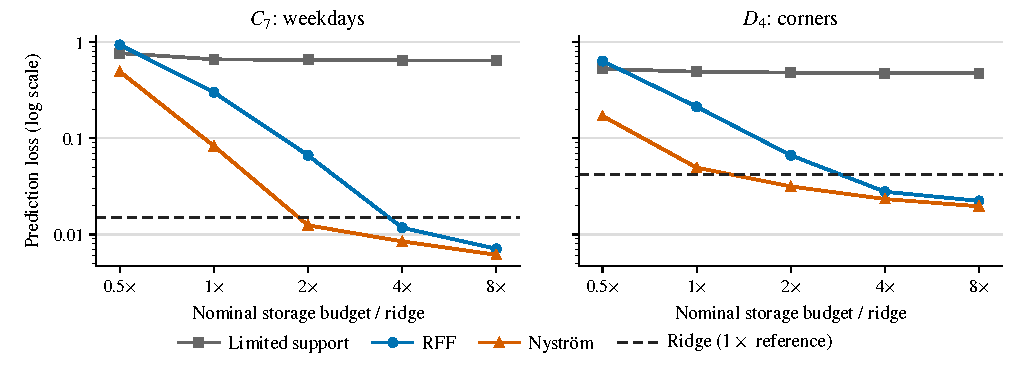
\includegraphics[width=\textwidth]{figures/budget_frontier.pdf}
\caption{\textbf{Predictor rankings change with storage.} Recorded direct-prediction means for all nonidentity actions on changed states under the specified semantic registration, over 24 fixed model/readout cells per domain. Losses use the Study~2 compact-comparison training-coordinate-energy denominator; lower is better. The horizontal axis is the nominal incremental parameter-storage budget relative to identity-pruned ridge, not runtime memory or statistical capacity. All five declared budgets and all three budgeted predictor families are shown. Nystr\"om first improves the group mean over ridge at $2\times$, and RFF at $4\times$, in both groups. Lines connect recorded aggregates on logarithmic axes; they are not fitted scaling laws or confidence bands. This direct-prediction endpoint is distinct from generator-only composition.}
\label{fig:budget-frontier}
\end{figure}

\subsection{Detailed interpretation questions}
\label{app:detailed-reading-protocol}
The findings motivate four complementary questions, conditional on states, contexts, coordinates, estimator and outcome. They organize interpretation rather than define a calibrated certification test or four statistically independent sources of evidence.

\paragraph{1. Predictive recovery.}
State what was held out: contexts, action elements, state identities or domains. Disclose comparator supervision and storage. Our generator result demonstrates why the distinction matters: transfer to an excluded action element can still use a completely familiar state vocabulary.

\paragraph{2. Action consistency.}
Specify the group-law residual, its metric and whether fitting encouraged it. The propagation identity relates consistency to prediction errors and operator norms. Additional semantic interpretation of these fitted diagnostics requires accounting for those quantities; separate objectives alone do not establish independent evidence. The same-bank class-risk comparison asks a different question by computing the independent linear and orthogonal optima and bounding the best exact-action risk under one common loss.

\paragraph{3. Preferential semantic alignment.}
Compare coherent alternatives as well as invalid registrations, making information, capacity, scoring rows, target definitions and predictive difficulty explicit. Our comparisons show why these controls answer different questions. Preference over selected alternatives would narrow the interpretation, rather than identify a unique semantic mechanism.

\paragraph{4. Native causal use.}
For a claim about successful native computation, establish clean-task competence and intervention fidelity, then distinguish sufficiency from necessity for the proposed mechanism. These activation edits illustrate the gap between moving an output score and identifying the computation used by the unedited model.

For a new application, specify the intended claim and competing explanation before choosing a diagnostic. The useful outcome is the interpretation changed by the comparison, including unfavorable results, rather than the number of positive scores obtained.


\FloatBarrier
\section{Independent Orthogonality and Further Common-Law Cost}
\label{app:orthogonal-results}
This completed comparison adds a same-bank class optimum to the original spectral analysis. It separates the computed cost of independent orthogonality from bounds on the further cost of a common exact action. It uses the original canonical semantic registration only; no new state, context, model, alternative-image search or witness fit is introduced. The primary $r=16$ results and the completed spectral sensitivity remain unchanged. All full-precision endpoints, zero lower bounds and numerical checks are retained in the accompanying supplement and public project.

\subsection{Observation and numerical contract}
The panel contains 48 fixed model/readout/domain conditions at each of $r=16$ and $r=8$, for 96 units. Each test bank has 128 complete context blocks, with seven weekday or four corner states. Dimension eight takes the first eight columns of the saved training-PCA coordinates in their original order. Each dimension uses its own uncentered empirical second moment $\Sigma=Z^\top Z/N$ and symmetric inverse-square-root whitening. There is no extra recentering, PCA refit, new direction, jitter, pseudoinverse or rank reduction. States, context blocks and all group elements receive uniform weights; identity actions and fixed points are included.

The second moment must satisfy the original strict rule $\lambda_{\min}/\lambda_{\max}>10^{-10}$. Matrix identities use the original normalized Frobenius tolerance $10^{-8}$; scalar comparisons use $10^{-8}+10^{-7}\max(|a|,|b|)$. Singular values and risks are retained without clipping. The only clipping in the reported law interval is the mathematical definition $\ell^-=\max(0,L_{\rm lower}-L_{\rm orth})$. Original archive hashes, member identities, model/tokenizer revisions, PCA identities and complete state/template rows bind each input. The fixed runtime was Python 3.11 with NumPy 2.2.6. In the accompanying cell-summary CSV, \texttt{sigma\_min}, \texttt{sigma\_max} and their ratio describe eigenvalues of the unwhitened second moment $\Sigma$.

For each action, compute $M_g=\mathbb E[x^\top x_g]$ by averaging the outer product over the complete state and context bank. If $M_g=U_g^{\rm svd}\operatorname{diag}(\sigma_{g,j})(V_g^{\rm svd})^\top$, one $O(r)$ optimum is $Q_g=U_g^{\rm svd}(V_g^{\rm svd})^\top$. No determinant correction is applied; the admissible class is $O(r)$, including reflections. A singular cross-moment may admit multiple optimal completions; the risk comparison does not identify a unique map. Direct residual risks are checked against
\[
 \eta=\frac{1}{r|G|}\sum_{g,j}(1-\sigma_{g,j}^2),\quad
 L_{\rm orth}=\frac{2}{r|G|}\sum_{g,j}(1-\sigma_{g,j}),\quad
 \beta=\frac{1}{r|G|}\sum_{g,j}(1-\sigma_{g,j})^2.
\]
Here $\eta$ and $L_{\rm orth}$ are class optima on the complete bank used for their calculation, and $\beta=L_{\rm orth}-\eta$ is their difference. They are not training-fitted prediction errors scored on a different bank. The existing $\gamma_r$, $L_{\rm lower}$ and $L_{\rm upper}$ are read from authenticated saved endpoints. They are not re-estimated for this comparison. Independently computed $\eta$, identity risk and second-moment diagnostics must match the saved values under the original checks.

Eight numerical software fixtures passed before the completed analysis, covering an analytic nonzero orthogonality cost, an exact reflection, singular cross-moments, row-vector orientation, deficient moments and invalid weight/masking/nonfinite inputs. All 96 units then completed, with 11,520 recorded checks passing. The two source archives had identical hashes before and after execution. Those are implementation and preservation checks, not calibrated statistical tests or rigorous floating-point enclosures. This manuscript integration reads the completed outputs without repeating tests or analysis.

\subsection{Magnitude, concentration and zero lower endpoints}
\Cref{tab:core-risk-summary}b reports the saved equal-cell means. The quantities of interest are
\[
 L^\star-\eta=\beta+(L^\star-L_{\rm orth}),\qquad
 \ell^-=\max(0,L_{\rm lower}-L_{\rm orth}),\qquad
 \ell^+=L_{\rm upper}-L_{\rm orth}.
\]
Every $\ell^\pm$ is formed per cell before averaging. In particular, averaging a clipped endpoint differs from clipping a difference of domain means. The exact costs decompose additively. Combining the computed orthogonality cost with the further-law lower endpoint gives the joint lower bound $\beta+\ell^-=\max(\beta,p^-)$, cell by cell. The corresponding upper endpoint is unchanged: $\beta+\ell^+=p^+$. The fraction of the true joint cost due to orthogonality depends on the unknown $L^\star$, rather than the lower endpoint $p^-$.

For $r=16$ C7, the additional-law lower endpoint has median $5.34554\times10^{-6}$ and range $[0,0.02618766]$. Its mean is $0.00109725$, and Llama-3.1-8B at layer 13 contributes $99.4445\%$ of its sum. The condition is retained at its original weight. This is concentration of the \emph{computed bounds}, not of the unknown true additional costs. It is a different quantity from the original joint lower endpoint $p^-$, whose sum has a $90.7\%$ contribution from two C7 conditions. For $r=16$ D4, the additional-law lower median is $0.000338944$ and the range is $[0,0.01261663]$; the largest condition contributes $28.5426\%$ of the sum. Upper bounds in both domains can remain much larger, so small lower bounds do not establish small optimal costs or practical equivalence.

At $r=8$, C7's additional-law lower median is $0.000778193$, with range $[0,0.11416052]$; D4's is $1.30864\times10^{-5}$, with range $[0,0.000401239]$. The smallest threshold-exceeding eight-coordinate C7 lower endpoint is $1.5462046788761175\times10^{-8}$, for Qwen2.5-3B at layer 7, only about $1.55$ times the unchanged software tolerance. It remains in the declared count; no threshold is adjusted retrospectively. These checks do not supply rigorous rounding-error certificates.

The nine computed zero lower endpoints are retained. At $r=16$ they occur for C7 in Llama-3.2-3B at layer 11, and for D4 in Qwen2.5-7B at layer 6. At $r=8$, the C7 cases are Qwen2.5-1.5B and Qwen2.5-7B at layer 6. The five D4 cases are Qwen2.5-7B at layer 22, Llama-3.1-8B at layer 13, Llama-3.2-1B at layer 13, and Llama-3.2-3B at layers 17 and 22. Zero is an inconclusive lower bound on strict positivity, not evidence that group laws have no cost. All 96 conditions remain in every relevant aggregate.

Each dimension changes the observation space, whitening and $1/r$ normalization. The two panels therefore do not select an optimal dimension or establish a common-metric improvement. The comparison concerns only the canonical action and does not rerank alternative images, re-evaluate frozen-witness transfer or add a semantic/native-computation claim. The full-precision table inputs, input mapping, checksums and formatting-only script are under \texttt{supplementary/orthogonal\_comparator}; complete per-cell summaries and the executed source bindings are retained in the public project.

\subsection{C7 context-family deletion sensitivity}
\label{app:c7-family-influence}
The concentration across model/readout conditions above does not establish concentration in a particular context family. We therefore examine whether removing any one family changes the additional-law lower bound in the original C7 bank. This completed, post-hoc analysis includes all 24 canonical-action conditions at $r=16$ and all 64 families. Each deletion removes both variants and their complete seven-state blocks, leaving 63 equally weighted families and 126 contexts. All states and all seven group elements, including identity, retain uniform weights. The original PCA basis, training mean, state correspondence, dimension and numerical tolerances remain fixed.

For each reduced bank, the unchanged spectral and independent-orthogonal kernels recompute its own \emph{uncentered} second moment and whitening, then evaluate $\eta$, $L_{\rm orth}$, $\gamma_r$ and the resulting constraint-cost bounds. Thus deletion changes both the empirical distribution and its metric, including the corresponding orthogonal-action class in the original coordinates. Differences are not additive family contributions under a fixed common metric. No extra centering, regularization, rank repair, historical-operator retraining or model forward pass is performed.

Twelve synthetic numerical tests passed, including closed-form risks, an independent Fourier-budget check, complete-family deletion and rank-failure cases. All 24 complete-bank baselines matched the saved results under the original rules before the 1,536 deletions were evaluated; all deletions completed. The analysis used Python 3.11.8 and NumPy 2.4.0, compared with NumPy 2.2.6 in the earlier orthogonal comparison. Baseline scalar discrepancies were at most $1.09\times10^{-14}$ without changing tolerances. The smallest reduced-bank second-moment eigenvalue ratio was $0.0039445$, above the original strict threshold $10^{-10}$. These are numerical validation checks, not rigorous floating-point certificates.

\begin{table}[t]
\caption{C7 family-deletion sensitivity of the further-law lower endpoint $\ell^-$, at $r=16$, in all 24 model/readout conditions. Minima and maxima cover all 64 complete-family deletions, each with its own empirical whitening; they are not confidence intervals. The final column counts endpoints satisfying $\ell^->10^{-8}+10^{-7}|\ell^-|$, out of 64. Zero is an inconclusive bound on strict positivity. Values are rounded only for display; full-precision endpoints and family identities are retained.}
\label{tab:c7-family-influence}
\centering\small
\setlength{\tabcolsep}{5pt}
\begin{tabular}{@{}lrrrrr@{}}
\toprule
Model & Layer & Baseline $\ell^-$ & Deletion min. & Deletion max. & \shortstack{Above tol.\\(/64)} \\
\midrule
Llama-3.2-1B & 3 & $3.540\times10^{-6}$ & $3.372\times10^{-6}$ & $4.079\times10^{-6}$ & 64/64 \\
 & 6 & $5.845\times10^{-6}$ & $5.252\times10^{-6}$ & $7.128\times10^{-6}$ & 64/64 \\
 & 10 & $1.128\times10^{-5}$ & $1.006\times10^{-5}$ & $1.374\times10^{-5}$ & 64/64 \\
 & 13 & $1.134\times10^{-5}$ & $1.047\times10^{-5}$ & $1.267\times10^{-5}$ & 64/64 \\
\addlinespace[2pt]
Llama-3.2-3B & 6 & $5.537\times10^{-6}$ & $5.307\times10^{-6}$ & $6.083\times10^{-6}$ & 64/64 \\
 & 11 & $0$ & $0$ & $0$ & 0/64 \\
 & 17 & $5.155\times10^{-6}$ & $4.104\times10^{-6}$ & $6.115\times10^{-6}$ & 64/64 \\
 & 22 & $2.595\times10^{-6}$ & $2.419\times10^{-6}$ & $2.914\times10^{-6}$ & 64/64 \\
\addlinespace[2pt]
Llama-3.1-8B & 6 & $2.058\times10^{-6}$ & $1.825\times10^{-6}$ & $2.406\times10^{-6}$ & 64/64 \\
 & 13 & $2.619\times10^{-2}$ & $2.435\times10^{-2}$ & $2.696\times10^{-2}$ & 64/64 \\
 & 19 & $6.538\times10^{-6}$ & $5.935\times10^{-6}$ & $7.448\times10^{-6}$ & 64/64 \\
 & 26 & $1.043\times10^{-5}$ & $9.416\times10^{-6}$ & $1.168\times10^{-5}$ & 64/64 \\
\addlinespace[2pt]
Qwen2.5-1.5B & 6 & $7.617\times10^{-6}$ & $7.267\times10^{-6}$ & $8.161\times10^{-6}$ & 64/64 \\
 & 11 & $1.238\times10^{-5}$ & $1.141\times10^{-5}$ & $1.370\times10^{-5}$ & 64/64 \\
 & 17 & $4.557\times10^{-6}$ & $4.209\times10^{-6}$ & $5.362\times10^{-6}$ & 64/64 \\
 & 22 & $6.010\times10^{-7}$ & $5.600\times10^{-7}$ & $7.323\times10^{-7}$ & 64/64 \\
\addlinespace[2pt]
Qwen2.5-3B & 7 & $6.462\times10^{-7}$ & $6.181\times10^{-7}$ & $7.216\times10^{-7}$ & 64/64 \\
 & 14 & $1.361\times10^{-5}$ & $1.127\times10^{-5}$ & $1.499\times10^{-5}$ & 64/64 \\
 & 22 & $2.747\times10^{-5}$ & $2.539\times10^{-5}$ & $2.914\times10^{-5}$ & 64/64 \\
 & 29 & $1.433\times10^{-6}$ & $1.342\times10^{-6}$ & $1.599\times10^{-6}$ & 64/64 \\
\addlinespace[2pt]
Qwen2.5-7B & 6 & $1.454\times10^{-6}$ & $9.852\times10^{-7}$ & $2.429\times10^{-6}$ & 64/64 \\
 & 11 & $6.239\times10^{-6}$ & $5.431\times10^{-6}$ & $7.513\times10^{-6}$ & 64/64 \\
 & 17 & $4.006\times10^{-6}$ & $3.560\times10^{-6}$ & $4.579\times10^{-6}$ & 64/64 \\
 & 22 & $1.933\times10^{-6}$ & $1.236\times10^{-6}$ & $2.487\times10^{-6}$ & 64/64 \\
\bottomrule
\end{tabular}

\end{table}
\FloatBarrier

\Cref{tab:c7-family-influence} reports every condition. The same 23 conditions exceed the original tolerance after every deletion; Llama-3.2-3B/layer 11 retains a zero lower endpoint throughout. Across the 64 common-family deletions, the equal-cell mean $\ell^-$ ranges from $0.00102081$ to $0.00112915$, compared with $0.00109725$ on the complete bank; the mean upper endpoint ranges from $0.02970592$ to $0.03043969$. Llama-3.1-8B/layer 13 remains the largest contributor, with $\ell^-\in[0.02434807,0.02695796]$ versus $0.02618766$ originally. Deleting family 016 gives its largest reduction, about $7.02\%$; deleting family 044 gives its largest increase, about $2.94\%$. Its share of the lower-endpoint sum remains $99.3822\%$--$99.4776\%$. The computed lower endpoint remains positive in this condition after each deletion, and its share of the sum stays above 99\%. These statements concern the lower endpoints.

This sensitivity check supports stability to the declared single-family deletions, while leaving multiple-family effects and shared language-construction biases unresolved. It is not independent-context replication, population inference or evidence about native computation. It does not evaluate alternative registrations: the optional all-image registration LOFO described in \cref{app:bounded-margin-details} remains prepared and unexecuted. The source supplement under \texttt{supplementary/c7\_family\_influence\_v1} retains the complete scalar outputs, input mapping and table formatter; the public project also retains all per-deletion diagnostics and the unchanged executed code. This manuscript revision integrates those completed records without rerunning numerical tests or analysis.


\FloatBarrier
\section{Retained Spectral and Joint-Premium Summaries}
\label{app:retained-summaries}
The main text combines same-bank risks and constraint costs in \cref{tab:core-risk-summary}. For continuity with the complete cell-level results, this appendix retains the original separate spectral and joint-premium summaries. The retained joint-premium tables report the original $p^-$, rather than the strengthened lower endpoint $\beta+\ell^-=\max(\beta,p^-)$ obtained from the independent-orthogonal comparison in \cref{app:orthogonal-results}. These tables use each original Study~2 test bank's own second-moment-whitened metric; they are distinct from the frozen-training-metric transfer comparison in \cref{tab:followup-witness}.

\begin{table}[H]
\caption{Finite-bank exact-action bounds in the test-bank metric. Each domain has 24 model/readout cells at $r=16$. The bounds concern cell-specific $L^\star$ over the entire exact orthogonal-action class in each test bank's own second-moment-whitened metric; displayed endpoints average those bounds, not confidence limits. $b_{\rm triv}$ is selected trivial-type energy divided by $r$. The last column counts unique highest-$\gamma_r$ ranks of the specified image among 120 C7 or three D4 images; it is not a rank of exact $L^\star$ or a significance test.}
\label{tab:followup-spectral}
\centering\small
\begin{tabular}{@{}lrrrrr@{}}
\toprule
Domain & Mean $\gamma_r$ & Mean bound endpoints & Mean $\eta$ & Mean $b_{\rm triv}$ & Image rank 1 \\
\midrule
$C_7$ & 0.98510 & [0.02980, 0.05863] & 0.02563 & 0.61540 & 7/24 \\
$D_4$ & 0.93528 & [0.12944, 0.24895] & 0.10321 & 0.72742 & 16/24 \\
\bottomrule
\end{tabular}
\end{table}


\begin{table}[H]
\caption{Same-metric reference and class-risk premium at $r=16$ on the original Study~2 test bank. Each domain averages \BoundedCellsPerDomain{} fixed cells equally. $p^-=\max\{0,2(1-\gamma_r)-\eta\}$ and $p^+=2(1-\gamma_r^2)-\eta$ are computed per cell before averaging. They bound the mean cost of imposing exact laws and orthogonality jointly. $L(I)$ uses total trivial energy and was also checked by direct residuals on the saved coordinates. These are finite-bank quantities, not transfer losses or confidence limits.}
\label{tab:bounded-risk}
\centering\small
% Generated by analysis/main30_bounded_v1/derive.py; never edit numbers.
\begin{tabular}{lrrrr}
\toprule
Domain & Mean $\eta$ & Mean $L(I)$ & Mean $p^-$ & Mean $p^+$ \\
\midrule
C7 & 0.02563 & 0.76012 & 0.00416 & 0.03300 \\
D4 & 0.10321 & 0.52932 & 0.02624 & 0.14574 \\
\bottomrule
\end{tabular}

\end{table}

\end{document}
